\documentclass[11pt,a4paper]{article}

% ---------- Idioma, fuente y página ----------
\usepackage[utf8]{inputenc}
\usepackage[T1]{fontenc}
\usepackage[spanish,es-noshorthands,es-tabla]{babel}
\usepackage{newtxtext,newtxmath}
\usepackage[a4paper,top=3.6cm,bottom=2.5cm,left=2.5cm,right=2.5cm,headheight=70pt,headsep=14pt]{geometry}
\usepackage{microtype}

% ---------- Paquetes ----------
\usepackage{graphicx}
\usepackage{pdfpages}
\usepackage[table]{xcolor}
\usepackage{needspace}
\usepackage{tabularx,longtable,booktabs,array,multirow}
\usepackage{enumitem}
\usepackage{float}
\usepackage{caption}
\usepackage{tikz}
\usetikzlibrary{shapes.geometric,arrows.meta,positioning,fit,calc,shapes.misc}
\usepackage{pgfplots}
\pgfplotsset{compat=1.18}
\usepackage{fancyhdr}
\usepackage{titlesec}
\usepackage{tocloft}
\usepackage[hidelinks]{hyperref}

\graphicspath{{../capturas/}{../img/}}
\setlength{\parindent}{0pt}
\setlength{\parskip}{6pt}
\renewcommand{\arraystretch}{1.25}
\captionsetup{font=small,labelfont=it,textfont=it,labelsep=period}
\captionsetup[figure]{name=Figura}
\captionsetup[table]{name=Tabla}
\setlist[itemize]{leftmargin=1.4em,itemsep=2pt,topsep=2pt,label=\small$\blacksquare$}
\setlist[enumerate]{leftmargin=1.6em,itemsep=2pt,topsep=2pt}
\definecolor{grisTarjeta}{HTML}{E6E6E6}
\definecolor{grisBorde}{HTML}{9A9A9A}

% ---------- Encabezado institucional (igual al Sprint 2) ----------
\pagestyle{fancy}
\fancyhf{}
\fancyhead[C]{%
  \begin{minipage}[c]{0.13\textwidth}
\includegraphics[width=1.5cm]{logo-izq.png}\end{minipage}%
  \begin{minipage}[c]{0.74\textwidth}\centering
    {\bfseries UNIVERSIDAD TÉCNICA DE AMBATO}\\[1pt]
    {\scriptsize\bfseries FACULTAD DE INGENIERÍA EN SISTEMAS ELECTRÓNICA E INDUSTRIAL}\\[1pt]
    {\scriptsize\bfseries CARRERA DE SOFTWARE}\\[1pt]
    {\scriptsize\bfseries CICLO ACADÉMICO: JULIO -- DICIEMBRE 2026}
  \end{minipage}%
  \begin{minipage}[c]{0.13\textwidth}\raggedleft
\includegraphics[width=1.5cm]{logo-der.png}\end{minipage}}
\fancyfoot[R]{\thepage}
\renewcommand{\headrulewidth}{1.2pt}

% ---------- Títulos de sección ----------
\titleformat{\section}{\normalfont\large\bfseries}{\thesection.}{0.5em}{\MakeUppercase}
\titleformat{\subsection}{\normalfont\normalsize\bfseries}{\thesubsection}{0.6em}{}
\titleformat{\subsubsection}{\normalfont\normalsize\bfseries\itshape}{}{0em}{}
\titlespacing*{\section}{0pt}{12pt}{6pt}
\titlespacing*{\subsection}{0pt}{10pt}{4pt}

% ---------- Índice "CONTENIDO" ----------
\addto\captionsspanish{\renewcommand{\contentsname}{CONTENIDO}}
\renewcommand{\cftsecleader}{\cftdotfill{\cftdotsep}}
\renewcommand{\cftsecaftersnum}{.}
\setlength{\cftbeforesecskip}{3pt}
\renewcommand{\listfigurename}{ÍNDICE DE FIGURAS}
\renewcommand{\listtablename}{ÍNDICE DE TABLAS}

% ---------- Tarjeta de historia de usuario ----------
% \historia{numero}{usuario}{nombre}{prioridad}{riesgo}{puntos}{iteracion}{responsables}{descripcion}{criterios}{observaciones}{mockups}
% LaTeX admite hasta 9 parámetros: \historia guarda los 9 primeros y \historiaFin recibe los 3 últimos.
\newcommand{\historia}[9]{%
\def\hNum{#1}\def\hUsu{#2}\def\hNom{#3}\def\hPri{#4}\def\hRie{#5}\def\hPun{#6}\def\hIte{#7}\def\hRes{#8}\def\hDes{#9}%
\historiaFin}
\newcommand{\historiaFin}[3]{%
\par\noindent
\begin{tabularx}{\textwidth}{|X|X|}
\hline
\rowcolor{grisTarjeta}\multicolumn{2}{|l|}{\large\textbf{Historia de Usuario}}\\\hline
\textbf{Número:} \hNum & \textbf{Usuario:} \hUsu\\\hline
\multicolumn{2}{|p{\dimexpr\textwidth-2\tabcolsep}|}{\textbf{Nombre historia:} \hNom}\\\hline
\textbf{Prioridad en negocio:} \hPri & \textbf{Riesgo en desarrollo:} \hRie\\\hline
\textbf{Puntos estimados:} \hPun & \textbf{Iteración asignada:} \hIte\\\hline
\multicolumn{2}{|p{\dimexpr\textwidth-2\tabcolsep}|}{\textbf{Programador responsable:} \hRes}\\\hline
\multicolumn{2}{|p{\dimexpr\textwidth-2\tabcolsep}|}{\textbf{Descripción:}\newline \hDes}\\\hline
\multicolumn{2}{|p{\dimexpr\textwidth-2\tabcolsep}|}{\textbf{Validación (criterios de aceptación):}\begin{itemize}#1\end{itemize}}\\\hline
\multicolumn{2}{|p{\dimexpr\textwidth-2\tabcolsep}|}{\textbf{Observaciones:} #2}\\\hline
\multicolumn{2}{|p{\dimexpr\textwidth-2\tabcolsep}|}{\textbf{Mockups / pantallas asociadas:} #3}\\\hline
\end{tabularx}\par\medskip}

% ---------- Tarjeta de tarea ----------
% \tarea{numero}{historia}{nombre}{tipo: D, C, M u O}{horas}{inicio}{fin}{responsable}{descripcion}
\newcommand{\marca}[2]{\ifx#1#2$\boxtimes$\else$\square$\fi}
\newcommand{\tarea}[9]{%
\par\noindent
\begin{tabularx}{\textwidth}{|X|X|}
\hline
\rowcolor{grisTarjeta}\multicolumn{2}{|l|}{\textbf{Tarea}}\\\hline
\textbf{Número tarea:} #1 & \textbf{Número historia:} #2\\\hline
\multicolumn{2}{|p{\dimexpr\textwidth-2\tabcolsep}|}{\textbf{Nombre tarea:} #3}\\\hline
\textbf{Tipo de tarea:} \marca{#4}{D} Desarrollo \marca{#4}{C} Corrección \marca{#4}{M} Mejora \marca{#4}{O} Otra & \textbf{Horas estimadas:} #5\\\hline
\textbf{Fecha inicio:} #6 & \textbf{Fecha fin:} #7\\\hline
\multicolumn{2}{|p{\dimexpr\textwidth-2\tabcolsep}|}{\textbf{Programador responsable:} #8}\\\hline
\multicolumn{2}{|p{\dimexpr\textwidth-2\tabcolsep}|}{\textbf{Descripción:} #9}\\\hline
\end{tabularx}\par\medskip}

% ---------- Diagrama de casos de uso (actor dibujado como muñeco, igual que en el Sprint 2) ----------
\definecolor{grisCaso}{HTML}{E4E8F0}
\tikzset{cu/.style={draw,ellipse,fill=grisCaso,align=center,font=\small,minimum width=4.1cm,minimum height=1cm,inner sep=1pt},
  rel/.style={densely dashed,-{Stealth[length=2mm]},font=\scriptsize}}
% \munieco{nombre}{(x,y)}{etiqueta}: crea los puntos nombre-e (derecha) y nombre-w (izquierda) para unir líneas.
\newcommand{\munieco}[3]{%
  \begin{scope}[shift={#2}]
    \draw[line width=0.9pt] (0,0.66) circle (0.18);
    \draw[line width=0.9pt] (0,0.48)--(0,-0.12) (-0.34,0.28)--(0.34,0.28) (0,-0.12)--(-0.28,-0.6) (0,-0.12)--(0.28,-0.6);
    \node[align=center,font=\small] at (0,-1.02) {#3};
    \coordinate (#1-e) at (0.42,0.2); \coordinate (#1-w) at (-0.42,0.2);
  \end{scope}}
\newcommand{\incluye}[2]{\draw[rel] (c#1) -- node[right]{«incluye»} (c#2);}
\newcommand{\extiende}[2]{\draw[rel] (c#1) -- node[right]{«extiende»} (c#2);}
% Relación entre casos que no están uno debajo del otro: se dibuja por el lado derecho.
\newcommand{\incluyeLado}[2]{\draw[rel] (c#1.east) to[out=-15,in=15,looseness=1.6] node[right]{«incluye»} (c#2.east);}
\newcommand{\extiendeLado}[2]{\draw[rel] (c#1.east) to[out=15,in=-15,looseness=1.6] node[right]{«extiende»} (c#2.east);}
% \casosdeuso{historia}{actor principal (vacío si se dibujan a mano)}{casos {a},{b},...}{casos unidos al actor}{dibujo extra}{explicación}
\newcommand{\casosdeuso}[6]{%
\par\needspace{12\baselineskip}\noindent\textbf{\textit{Diagrama de casos de uso -- #1}}\par
\begin{figure}[H]\centering
\begin{tikzpicture}
  \foreach \c [count=\i] in {#3} {\node[cu] (c\i) at (5.6,{-1.45*(\i-1)}) {\c}; \xdef\ncu{\i}}
  \node[font=\bfseries] (titulo) at (5.6,1.05) {Sistema de homologación};
  \node[draw,rounded corners=5pt,inner sep=8pt,fit=(titulo)(c1)(c\ncu)] {};
  \if\relax\detokenize{#2}\relax\else
    \munieco{act}{(0,{-0.725*(\ncu-1)})}{#2}
    \foreach \i in {#4} {\draw (act-e) -- (c\i.west);}
  \fi
  #5
\end{tikzpicture}
\caption{Diagrama de casos de uso de la #1}
\end{figure}
#6\par\medskip}

% ---------- Prueba con captura (formato de la sección de resultados del Sprint 2) ----------
% \prueba{titulo}{accion}{archivo}{pie de figura}{resultado obtenido}{ancho relativo}
\newcommand{\prueba}[6]{%
\par\needspace{0.5\textheight}%
{\bfseries\itshape #1}\par
\textbf{Acción:} #2\par
\begin{figure}[H]\centering
\includegraphics[width=#6\textwidth,height=0.55\textheight,keepaspectratio]{#3}
\caption{#4}
\end{figure}
\textbf{Resultado obtenido:} #5\par\bigskip}
\usepackage{needspace}

\begin{document}

% ---------- Portada (misma del Sprint 2, con el tema actualizado) ----------

\includepdf[pages=1]{../img/portada.pdf}

\setcounter{page}{2}
\begin{center}
{\large\bfseries I. INFORME}
\end{center}
\tableofcontents
\clearpage

\section{Introducción}
\subsection{Descripción del problema}
En la FISEI, la homologación de asignaturas requiere revisar planes analíticos, créditos y contenidos. La revisión manual demanda tiempo y puede dificultar la explicación de una resolución. La decisión académica corresponde al docente y debe conservar su criterio.

\subsection{Descripción del proyecto}
SIHA-IA (Sistema Inteligente de Homologación Académica) es una aplicación web para registrar solicitudes y apoyar su análisis mediante lectura documental, reglas configuradas y herramientas de inteligencia artificial local. El resultado sirve de apoyo para el personal académico; la decisión final es humana.

\subsection{Alcance de los Sprints 1, 2 y 3}
El Sprint 1 estableció la base: cuentas y roles, reglas, catálogo académico, API Gateway, expedientes y publicación de solicitudes. El Sprint 2 incorporó la lectura de planes, confirmación de datos dudosos, análisis de créditos y contenidos, y consulta de precedentes. El Sprint 3 integra el certificado SIHA único emitido por Secretaría, aplica la regla de créditos y contenidos aclarada con el docente, registra la decisión de docentes y administrador, considera movilidad externa, presenta una tabla de resultados y automatiza el registro manual del resultado.

\subsection{Objetivos}
\textbf{Objetivo general.} Apoyar el trámite de homologación con un sistema que registre y analice solicitudes y facilite una resolución académica trazable.

\textbf{Objetivos específicos.}
\begin{itemize}
\item Registrar expedientes y documentos, y conservar los datos de la solicitud.
\item Analizar créditos y contenidos según las reglas acordadas.
\item Presentar los hallazgos a docentes y permitir la resolución prevista por el flujo institucional.
\item Mantener el historial de resultados y decisiones.
\end{itemize}

\subsection{Marco normativo}
El proyecto considera los instructivos CAU-P-011, para cambio de carrera, y CAU-P-122, para movilidad. SIHA-IA apoya la revisión y el registro del caso, pero no sustituye el trámite ni la autoridad académica.

\subsection{Términos utilizados}
\begin{tabularx}{\textwidth}{|p{0.25\textwidth}|X|}\hline
\rowcolor{grisTarjeta}\textbf{Término} & \textbf{Significado en este informe}\\\hline
Certificado SIHA & Documento único emitido por Secretaría que contiene la información de la solicitud.\\\hline
Sílabo & Documento con información académica de una asignatura.\\\hline
Créditos & Valor académico asignado a una materia.\\\hline
Contenidos & Temas y unidades que se revisan para comparar asignaturas.\\\hline
Agente & Componente que procesa una solicitud y coordina el análisis.\\\hline
JWT & Token firmado que permite identificar la sesión y sus permisos.\\\hline
Gateway & Punto de entrada que valida y dirige las peticiones a los servicios.\\\hline
Microservicio & Servicio independiente que cumple una función del sistema.\\\hline
RabbitMQ & Servicio de mensajería usado para intercambiar eventos.\\\hline
Ollama & Herramienta que ejecuta modelos de inteligencia artificial localmente.\\\hline
CUMPLE & Resultado que indica que se alcanza la condición evaluada.\\\hline
NO\_CUMPLE & Resultado que indica que no se alcanza la condición evaluada.\\\hline
CRITERIO\_DOCENTE & Caso que requiere valoración y decisión de docentes.\\\hline
Bloqueada por créditos & Solicitud que no pasa a votación por no alcanzar el mínimo de créditos.\\\hline
\end{tabularx}
\captionof{table}{Términos utilizados}

\section{Justificación del stack tecnológico}
La selección mantiene las tecnologías de la solución y separa la interfaz, los servicios, los datos y la comunicación entre componentes.

\begin{tabularx}{\textwidth}{|p{0.18\textwidth}|p{0.32\textwidth}|X|}\hline
\rowcolor{grisTarjeta}\textbf{Capa} & \textbf{Tecnología} & \textbf{Justificación}\\\hline
Servicios & .NET 8 y ASP.NET Core & Plataforma para implementar servicios web con soporte de pruebas y despliegue.\\\hline
Persistencia & Entity Framework Core & Mapea entidades y administra cambios de esquema mediante migraciones.\\\hline
Datos & SQL Server A, B y C & Una base de datos por microservicio, para mantener separados sus datos.\\\hline
Mensajería & RabbitMQ y MassTransit & Publica y consume eventos entre servicios con reintentos.\\\hline
Enrutamiento & Ocelot & Centraliza la entrada HTTP y el direccionamiento hacia los servicios.\\\hline
Inteligencia artificial & Ollama y embeddings & Permite ejecutar modelos y comparar contenidos dentro del entorno local.\\\hline
Interfaz & React, Vite, TypeScript y Tailwind & Construye una interfaz web tipada y facilita el desarrollo y la presentación.\\\hline
Entorno & Docker Compose & Levanta los componentes relacionados en un entorno reproducible.\\\hline
Pruebas & xUnit y Vitest & Ejecutan pruebas automatizadas de backend y frontend.\\\hline
Integración & GitHub Actions & Automatiza compilación y validaciones del proyecto.\\\hline
\end{tabularx}
\captionof{table}{Tecnologías y justificación}

\section{Arquitectura del sistema}
\subsection{Descripción general}
SIHA-IA se compone de una interfaz web, un API Gateway y tres microservicios. El MS A administra usuarios, catálogo y reglas; el MS B registra expedientes y documentos; el MS C procesa el análisis. Cada microservicio dispone de su propia base SQL. RabbitMQ transporta eventos y Ollama proporciona modelos locales para el análisis.

\subsection{Flujo de una solicitud actual}
\begin{enumerate}
\item El operador registra la solicitud y carga el certificado SIHA.
\item La interfaz envía la petición al API Gateway, que valida el JWT y dirige la solicitud.
\item El MS B lee y valida el certificado y comprueba que las materias indicadas se relacionan.
\item El MS B guarda el expediente y publica el evento \texttt{SolicitudCreadaEvent} en RabbitMQ.
\item El MS C recibe el evento y analiza el expediente con los sílabos disponibles en el MS A y los modelos de Ollama.
\item Los docentes revisan la solicitud y registran sus votos.
\item Si los votos no coinciden, el administrador registra la decisión correspondiente.
\item El sistema conserva el resultado como \texttt{RESULTADO\_HOMOLOGACION}.
\end{enumerate}

\subsection{Diagrama de arquitectura}
\begin{figure}[H]\centering
\begin{tikzpicture}[node distance=0.9cm and 1.1cm, caja/.style={draw,rounded corners,align=center,minimum width=2.4cm,minimum height=0.85cm,font=\small}, db/.style={draw,cylinder,shape border rotate=90,aspect=0.25,align=center,minimum height=0.8cm,font=\small}, flecha/.style={-{Stealth},thick}]
\node[caja] (ui) {Interfaz web\\5173};
\node[caja,below=of ui] (gw) {API Gateway\\5000};
\node[caja,below left=1cm and 1.8cm of gw] (a) {MS A\\5081};
\node[caja,below=1cm of gw] (b) {MS B\\5082};
\node[caja,below right=1cm and 1.8cm of gw] (c) {MS C\\5084};
\node[db,below=of a] (da) {SQL A};
\node[db,below=of b] (dbb) {SQL B};
\node[db,below=of c] (dc) {SQL C};
\node[caja,right=2.3cm of b] (mq) {RabbitMQ};
\node[caja,below=of mq] (oll) {Ollama};
\draw[flecha] (ui)--node[right,font=\scriptsize]{HTTP / JWT}(gw);
\draw[flecha] (gw)--(a); \draw[flecha] (gw)--(b); \draw[flecha] (gw)--(c);
\draw[flecha] (a)--(da); \draw[flecha] (b)--(dbb); \draw[flecha] (c)--(dc);
\draw[flecha] (b)--node[above,font=\scriptsize]{evento}(mq);
\draw[flecha] (mq)--(c); \draw[flecha] (c)--node[right,font=\scriptsize]{análisis}(oll);
\draw[flecha,dashed] (c) to[bend left=20] node[above,font=\scriptsize]{gRPC: sílabos}(a);
\end{tikzpicture}
\caption{Arquitectura de SIHA-IA y puertos locales indicados en el despliegue}
\end{figure}

\section{Metodología Scrum + XP}
El equipo organiza el trabajo con Scrum y aplica prácticas de XP para construir y revisar el producto en incrementos. Se conserva la secuencia y el enfoque descritos en el informe del Sprint 2.

\subsection{Roles}
\begin{tabularx}{\textwidth}{|p{0.34\textwidth}|p{0.3\textwidth}|X|}\hline
\rowcolor{grisTarjeta}\textbf{Integrante} & \textbf{Rol} & \textbf{Responsabilidad}\\\hline
Jair León & Scrum Master / Backend & Facilita el trabajo del equipo y contribuye al backend.\\\hline
Paul Acurio & Product Owner Proxy / IA & Prioriza y aclara necesidades; apoya el análisis con IA.\\\hline
Alex Jonathan Chisag & Frontend / UI-UX & Implementa la interfaz y revisa la experiencia de uso.\\\hline
Rolando Sebastián Miranda & Backend / QA-DevOps & Apoya servicios backend, calidad e infraestructura.\\\hline
Ing. Hernán Naranjo, Mg. & Docente & Acompaña y revisa el trabajo académico.\\\hline
\end{tabularx}
\captionof{table}{Roles del equipo}

\subsection{Eventos y artefactos}
Se realizan planificación, reuniones diarias, revisión y retrospectiva. Los artefactos de trabajo son el Product Backlog, el Sprint Backlog, el incremento y la definición de hecho. El equipo revisa el avance y actualiza las tareas conforme a los acuerdos del sprint.

\subsection{Prácticas XP}
Se aplican pruebas automáticas, integración continua, programación en parejas o revisión de código, refactorización, entregas pequeñas, ramas de trabajo y solicitudes de cambios (PR). Estas prácticas ayudan a detectar errores durante el desarrollo y a integrar cambios revisables.

\subsection{Definición de Hecho}
Una historia se considera terminada cuando cumple sus criterios de aceptación, sus pruebas relevantes pasan, el cambio queda integrado y revisado, y la funcionalidad puede demostrarse con el incremento del sistema.

\section{Sprint 1: base del sistema}
\subsection{Objetivo y alcance}
El Sprint 1 estableció la base técnica y funcional: cuentas y roles, reglas y umbrales, catálogo de carreras y asignaturas, entrada central mediante Gateway, registro de expedientes con PDF y publicación de solicitudes en RabbitMQ. La planificación original identificó las historias como US-01 a US-06; aquí se presentan con la nomenclatura HU-01 a HU-06.

\subsection{Sprint Backlog}
\begin{tabularx}{\textwidth}{|c|X|c|}\hline
\rowcolor{grisTarjeta}\textbf{Historia} & \textbf{Alcance} & \textbf{SP}\\\hline
HU-01 & Cuentas, autenticación y roles & 5\\\hline
HU-02 & Reglas y umbrales & 5\\\hline
HU-03 & Carreras, mallas y asignaturas & 5\\\hline
HU-04 & API Gateway (habilitadora) & 5\\\hline
HU-05 & Registrar expedientes y PDF & 8\\\hline
HU-06 & Publicar solicitudes en RabbitMQ (habilitadora) & 5\\\hline
\multicolumn{2}{|r|}{Total} & 33\\\hline
\end{tabularx}
\captionof{table}{Sprint Backlog del Sprint 1}

\subsection{Historias, criterios y tareas}
\subsubsection{HU-01: Cuentas y roles}
\historia{HU-01}{Administrador del sistema}{Gestión de cuentas y roles}{Alta}{Media}{5 SP}{Sprint 1}{Jair León; Paul Acurio; Alex Jonathan Chisag; Rolando Sebastián Miranda}{Como administrador, quiero crear y gestionar cuentas con roles, para que cada persona acceda solo a las funciones autorizadas.}{\item Dado un registro válido, cuando se crea una cuenta, entonces se asigna el rol solicitado y la contraseña se guarda como hash.\item Dado un usuario activo, cuando sus credenciales son correctas, entonces obtiene una sesión con su rol.\item Dado un rol sin permiso o un correo duplicado, cuando intenta gestionar cuentas, entonces la operación se rechaza.}{Historia denominada US-01 en la fuente.}{M-01 (Inicio de sesión institucional)}
\casosdeuso{HU-01}{Administrador}{{Iniciar sesión},{Crear cuenta con rol},{Validar correo único},{Activar o desactivar\\cuenta}}{1,2,4}{\incluye{2}{3}}{El administrador inicia sesión y gestiona las cuentas; al crear una cuenta siempre se valida que el correo no esté repetido.}
\par\needspace{8\baselineskip}\noindent\textbf{\textit{Desglose de tareas -- HU-01}}\par
La historia se divide en 7 tareas que suman 20,3 horas.\par\medskip
\tarea{S1-J01}{HU-01}{Definición de contratos REST y migraciones iniciales en DB A}{D}{2,9 h}{Día 1 del Sprint 1}{Día 1 del Sprint 1}{Jair Alexander León Tusa}{Definir los contratos REST de usuarios, reglas y catálogo académico, y generar las migraciones iniciales con Entity Framework Core para las tablas USUARIO y ROL en SQL Server DB A.}
\tarea{S1-S01}{HU-01}{Configuración de contenedores Docker Compose para bases de datos y servicios}{O}{2,9 h}{Día 1 del Sprint 1}{Día 1 del Sprint 1}{Rolando Sebastián Miranda Baño}{Configurar el archivo docker-compose.yml para levantar las instancias aisladas de SQL Server (DB A, DB B, DB C), RabbitMQ y los microservicios .NET Core 8 verificando conectividad de red.}
\tarea{S1-J02}{HU-01}{Implementación de alta de usuarios, hash BCrypt y gestión de estado/rol}{D}{2,9 h}{Día 2 del Sprint 1}{Día 2 del Sprint 1}{Jair Alexander León Tusa}{Implementar en el Microservicio A los endpoints de creación y actualización de cuentas, aplicando cifrado BCrypt a las contraseñas, validación de correo institucional único y control de estado activo/inactivo.}
\tarea{S1-S02}{HU-01}{Implementación de autenticación JWT con claims de rol y expiración}{D}{2,9 h}{Día 2 del Sprint 1}{Día 2 del Sprint 1}{Rolando Sebastián Miranda Baño}{Implementar el servicio emisor de tokens JWT firmados en el Microservicio A, inyectando los claims de identidad y rol ( ADMINISTRADOR, DOCENTE, OPERADOR ) y rechazando cuentas inactivas o credenciales inválidas.}
\tarea{S1-A02}{HU-01}{Construcción de vista de inicio de sesión y manejo de sesión en React}{D}{2,9 h}{Día 2 del Sprint 1}{Día 2 del Sprint 1}{Alex Jonathan Chisag Punina}{Desarrollar en React 18 + TypeScript la pantalla de acceso institucional, el almacenamiento seguro del token JWT en sesión y el bloqueo visual de rutas restringidas con pantalla de acceso denegado.}
\tarea{S1-P02}{HU-01}{Verificación de matriz de permisos RBAC por rol}{M}{2,9 h}{Día 2 del Sprint 1}{Día 2 del Sprint 1}{Paul Medardo Acurio López}{Revisar y ejecutar las pruebas de autorización para los roles Administrador, Docente y Operador sobre los endpoints de cuentas, documentando la matriz de accesos válidos ( 200/201) y denegados (401/403).}
\tarea{S1-S03}{HU-01}{Pruebas unitarias de autenticación RBAC en xUnit y esquema DB B}{C}{2,9 h}{Día 3 del Sprint 1}{Día 3 del Sprint 1}{Rolando Sebastián Miranda Baño}{Codificar pruebas unitarias en xUnit + Moq para validar el bloqueo RBAC y emisión JWT (1,7 h) y generar las migraciones iniciales de expedientes en SQL Server DB B (1,2 h).}
\par\needspace{14\baselineskip}\noindent\textbf{\textit{Mockup de HU-01}}\par
\begin{figure}[H]\centering\fbox{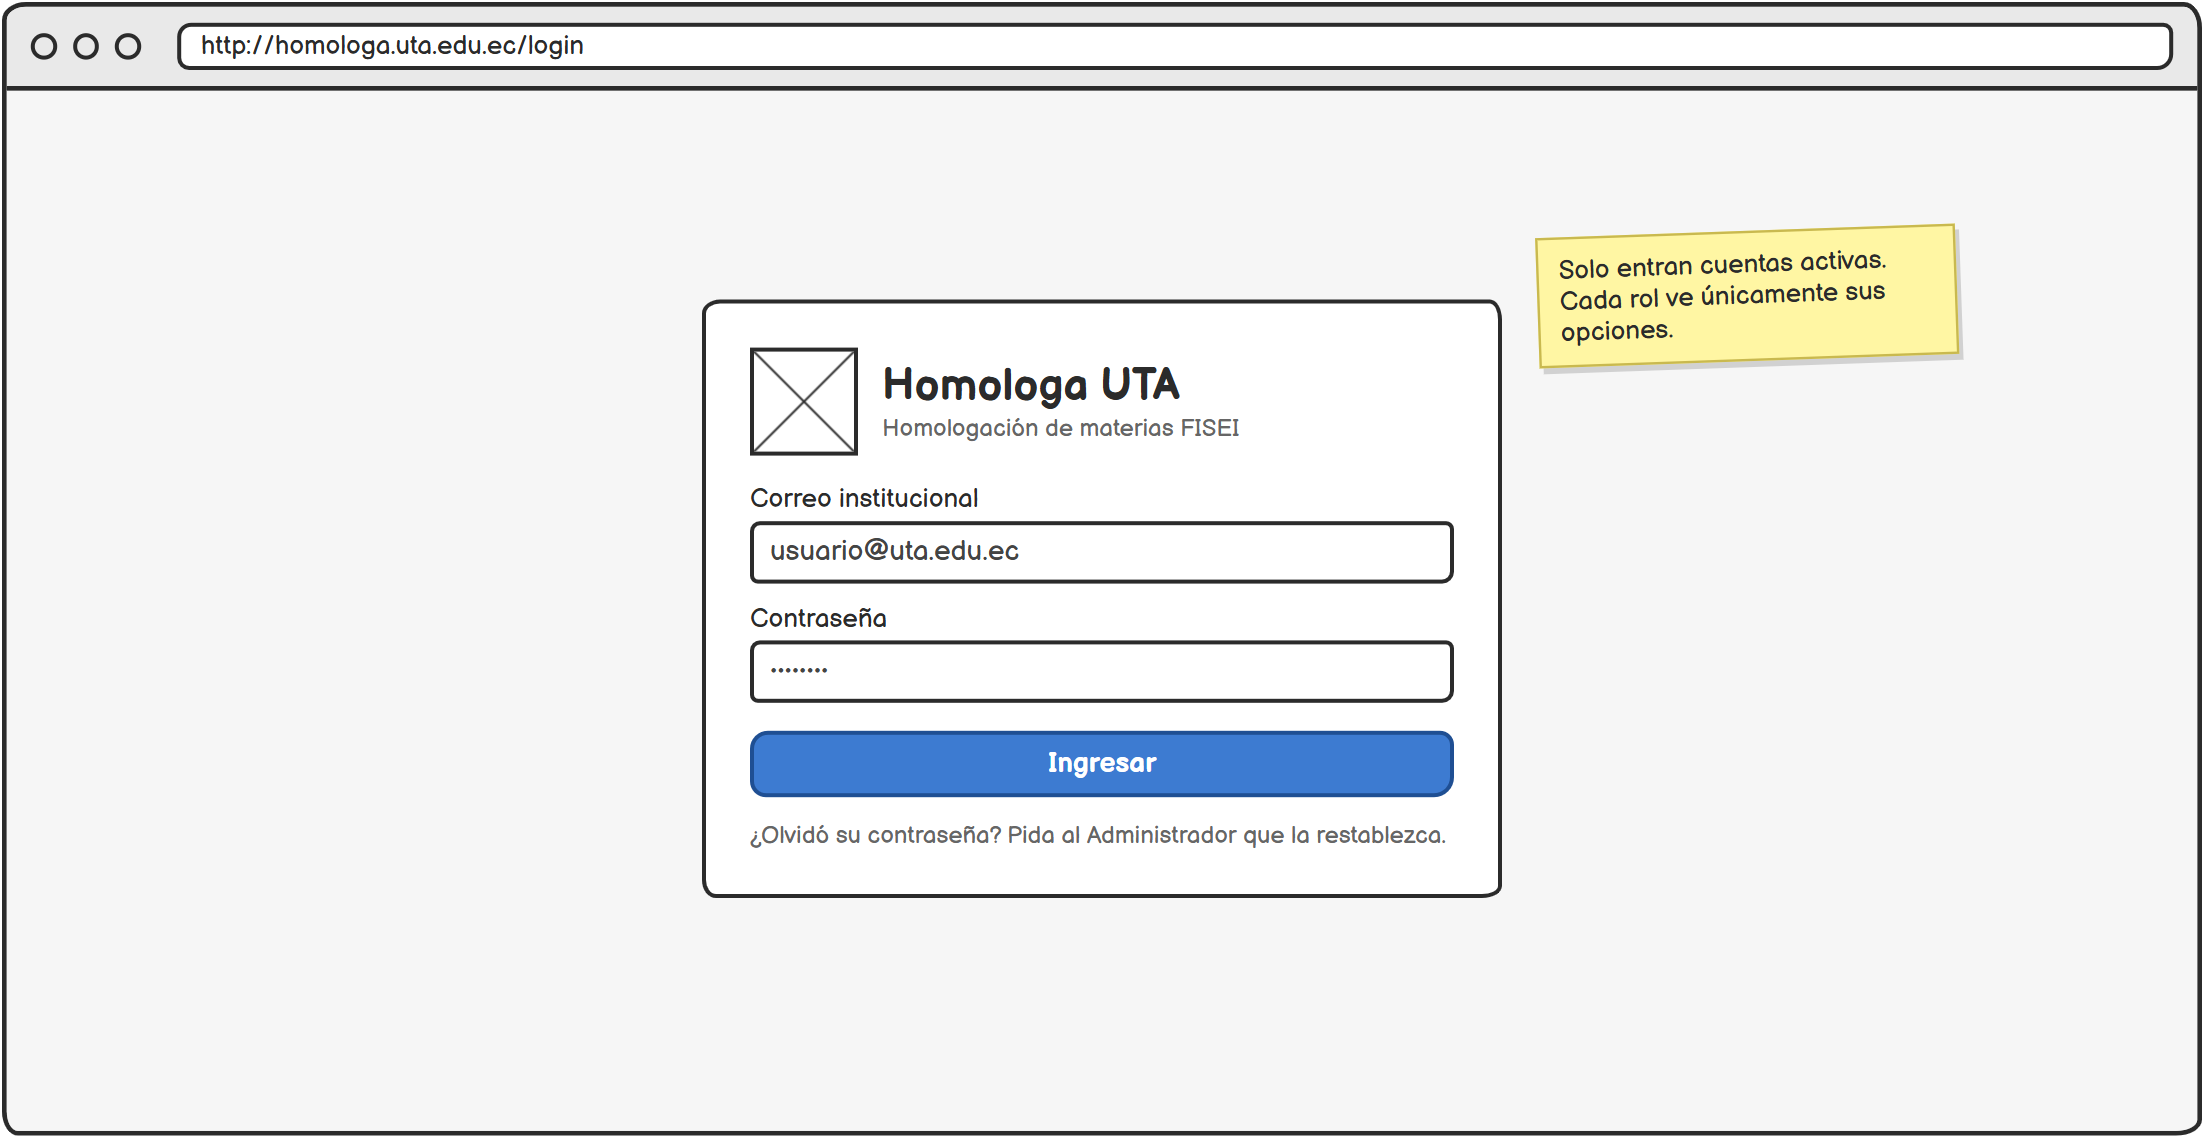
\includegraphics[width=0.93\textwidth]{mockups/m01.png}}
\caption{Mockup M-01 -- Inicio de sesión institucional}
\end{figure}
\par\needspace{6\baselineskip}\noindent\textbf{\textit{Pruebas de aceptación -- HU-01}}\par
\begin{longtable}{|p{1.4cm}|p{3.7cm}|p{4.6cm}|p{5.1cm}|}
\hline\rowcolor{grisTarjeta}\textbf{N.º} & \textbf{Prueba} & \textbf{Entrada} & \textbf{Resultado esperado}\\\hline
\endhead
PA-01.1 & Lista de cuentas con su rol y estado & El administrador abre Usuarios y roles. & Cuentas con rol, estado y acciones\\\hline
PA-01.2 & Crear una cuenta con datos que no coinciden & El administrador intenta crear una cuenta escribiendo dos contraseñas distintas. & ``Las contraseñas no coinciden''; no se crea\\\hline
PA-01.3 & Un rol sin permiso entra a Usuarios y roles & El operador escribe a mano la dirección de Usuarios y roles. & ``No tiene acceso a esta sección''\\\hline
\caption{Pruebas de aceptación de la HU-01}
\end{longtable}

\subsubsection{HU-02: Reglas y umbrales}
\historia{HU-02}{Administrador del sistema}{Reglas y umbrales configurables}{Alta}{Media}{5 SP}{Sprint 1}{Jair León; Paul Acurio; Alex Jonathan Chisag; Rolando Sebastián Miranda}{Como administrador, quiero configurar reglas y umbrales, para aplicar de forma consistente los criterios acordados.}{\item Dado un umbral válido, cuando se guarda, entonces queda asociado a su trámite, fuente y vigencia.\item Dado un valor fuera del rango permitido, cuando se actualiza, entonces se rechaza sin reemplazar la configuración vigente.\item Dado un usuario sin rol administrador, cuando modifica reglas, entonces se deniega la operación.}{La fuente la denomina US-02.}{M-02 (Configurar el mínimo para homologar)}
\casosdeuso{HU-02}{Administrador}{{Consultar reglas vigentes},{Cambiar el mínimo (80~\%)},{Guardar nueva versión},{Ver historial de versiones}}{1,2,4}{\incluye{2}{3}}{Cada cambio del mínimo se guarda como una nueva versión de la regla; el mínimo no puede bajar de 80~\%.}
\par\needspace{8\baselineskip}\noindent\textbf{\textit{Desglose de tareas -- HU-02}}\par
La historia se divide en 5 tareas que suman 14,5 horas.\par\medskip
\tarea{S1-J03}{HU-02}{Implementación de API REST de consulta y actualización de reglas y umbrales}{D}{2,9 h}{Día 3 del Sprint 1}{Día 3 del Sprint 1}{Jair Alexander León Tusa}{Implementar en el Microservicio A los endpoints REST para consultar y actualizar los umbrales de créditos y de contenidos y las reglas de cada trámite, validando que los valores estén en rango y que solo el Administrador pueda cambiarlos.}
\tarea{S1-A03}{HU-02}{Construcción del formulario web de reglas y parámetros de evaluación}{D}{2,9 h}{Día 3 del Sprint 1}{Día 3 del Sprint 1}{Alex Jonathan Chisag Punina}{Construir en React 18 el formulario de configuración de reglas con selector de ruta de trámite (CAU-P-011 / CAU-P-122), campos para los umbrales de créditos y contenidos, validaciones de rango y estados de guardado/error.}
\tarea{S1-P03}{HU-02}{Pruebas de validación de rangos y permisos en configuración de umbrales}{M}{2,9 h}{Día 3 del Sprint 1}{Día 3 del Sprint 1}{Paul Medardo Acurio López}{Probar la configuración de umbrales con valores válidos, valores fuera de rango (negativos, mayores que 100~\% o umbrales incoherentes entre sí) y peticiones con roles no autorizados, documentando las evidencias positivas y negativas.}
\tarea{S1-S04}{HU-02}{Implementación del servidor gRPC de reglas en Microservicio A}{D}{2,9 h}{Día 4 del Sprint 1}{Día 4 del Sprint 1}{Rolando Sebastián Miranda Baño}{Definir el contrato reglas.proto e implementar el servidor ReglasGrpc en el Microservicio A para exponer con baja latencia los umbrales vigentes hacia el Microservicio C.}
\tarea{S1-A08}{HU-02}{Integración de acceso, umbrales y catálogo con Microservicio A vía Gateway}{C}{2,9 h}{Día 8 del Sprint 1}{Día 8 del Sprint 1}{Alex Jonathan Chisag Punina}{Conectar los formularios de inicio de sesión, reglas y catálogo académico con los servicios reales del Microservicio A a través del API Gateway, retirando los mocks iniciales.}
\par\needspace{14\baselineskip}\noindent\textbf{\textit{Mockup de HU-02}}\par
\begin{figure}[H]\centering\fbox{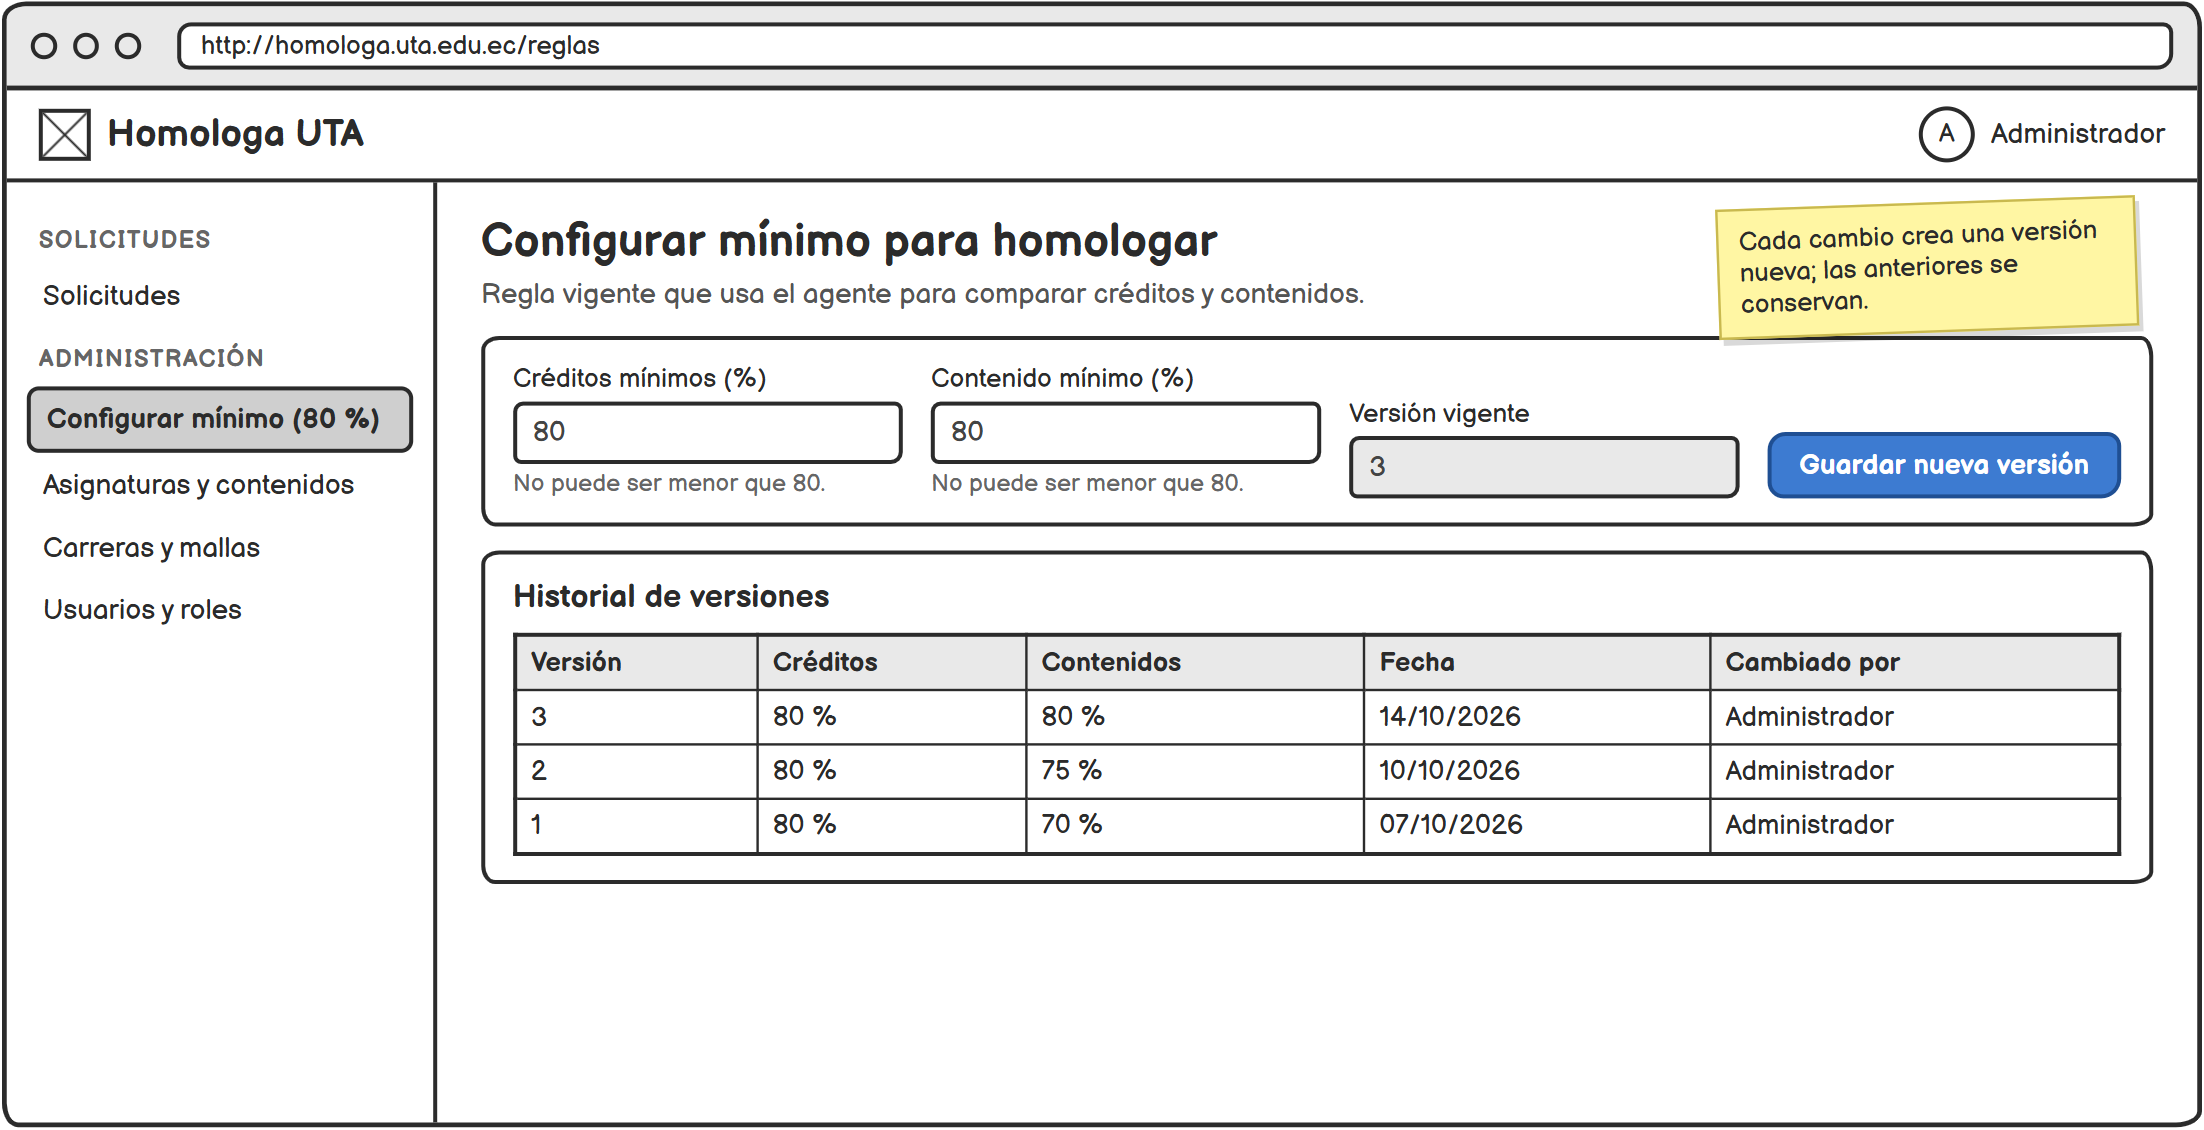
\includegraphics[width=0.93\textwidth]{mockups/m02.png}}
\caption{Mockup M-02 -- Configurar el mínimo para homologar}
\end{figure}
\par\needspace{6\baselineskip}\noindent\textbf{\textit{Pruebas de aceptación -- HU-02}}\par
\begin{longtable}{|p{1.4cm}|p{3.7cm}|p{4.6cm}|p{5.1cm}|}
\hline\rowcolor{grisTarjeta}\textbf{N.º} & \textbf{Prueba} & \textbf{Entrada} & \textbf{Resultado esperado}\\\hline
\endhead
PA-02.1 & Reglas vigentes y catálogo normativo & El administrador abre Configurar mínimo (80~\%). & Mínimo 80~\% y catálogo RN\\\hline
PA-02.2 & Intentar bajar el mínimo de 80~/~\% & El administrador escribe 70 en Contenido mínimo y guarda. & Rechazado con mensaje claro\\\hline
\caption{Pruebas de aceptación de la HU-02}
\end{longtable}

\subsubsection{HU-03: Carreras, mallas y asignaturas}
\historia{HU-03}{Administrador y operador}{Carreras, mallas y asignaturas}{Alta}{Media}{5 SP}{Sprint 1}{Jair León; Alex Jonathan Chisag; Paul Acurio}{Como administrador, quiero gestionar carreras, mallas y asignaturas, para que el operador pueda seleccionar las materias del caso.}{\item Dado un plan académico, cuando se consulta, entonces se identifican carrera, versión, asignatura, créditos, horas y unidades disponibles.\item Dado un código duplicado, cuando se carga, entonces el sistema lo rechaza.}{La fuente la denomina US-03.}{M-03 (Asignaturas de la malla)}
\casosdeuso{HU-03}{Administrador}{{Consultar carreras y mallas},{Registrar asignaturas\\por nivel},{Validar créditos y nivel},{Consultar contenidos\\de la asignatura}}{1,2,4}{\incluye{2}{3}}{Al registrar una asignatura siempre se validan sus créditos y su nivel dentro de la malla.}
\par\needspace{8\baselineskip}\noindent\textbf{\textit{Desglose de tareas -- HU-03}}\par
La historia se divide en 5 tareas que suman 14,5 horas.\par\medskip
\tarea{S1-J04}{HU-03}{Implementación de CRUD de carreras y versiones de mallas curriculares}{D}{2,9 h}{Día 4 del Sprint 1}{Día 4 del Sprint 1}{Jair Alexander León Tusa}{Implementar en el Microservicio A los controladores y servicios CRUD para las entidades CARRERA y MALLA, validando códigos únicos y relaciones en SQL Server DB A.}
\tarea{S1-A04}{HU-03}{Construcción de listado y formularios web de carreras y mallas}{D}{2,9 h}{Día 4 del Sprint 1}{Día 4 del Sprint 1}{Alex Jonathan Chisag Punina}{Desarrollar en React 18 las vistas de consulta y registro de carreras (Software, TI, Industrial, Robótica, Telecomunicaciones) y versiones de mallas curriculares.}
\tarea{S1-J05}{HU-03}{Implementación de CRUD de asignaturas, unidades e importación de 43 planes}{D}{2,9 h}{Día 5 del Sprint 1}{Día 5 del Sprint 1}{Jair Alexander León Tusa}{Implementar el CRUD de ASIGNATURA y UNIDAD\_TEMATICA y el cargador masivo del catálogo estructurado (43 planes analíticos de Software), validando créditos, horas por unidad y rechazo de duplicados.}
\tarea{S1-A05}{HU-03}{Construcción de interfaz de edición de asignaturas y carga estructurada}{D}{2,9 h}{Día 5 del Sprint 1}{Día 5 del Sprint 1}{Alex Jonathan Chisag Punina}{Completar en React la interfaz de gestión de asignaturas, unidades temáticas y el componente de importación del catálogo estructurado con resumen visual de validación y errores.}
\tarea{S1-P05}{HU-03}{Validación funcional de carga del catálogo, duplicados, créditos y horas}{M}{2,9 h}{Día 5 del Sprint 1}{Día 5 del Sprint 1}{Paul Medardo Acurio López}{Ejecutar pruebas de importación de los 43 planes analíticos de Software, verificando rechazo de códigos duplicados, equivalencia de 48 h/crédito UTA y marcado de planes incompletos.}
\par\needspace{14\baselineskip}\noindent\textbf{\textit{Mockup de HU-03}}\par
\begin{figure}[H]\centering\fbox{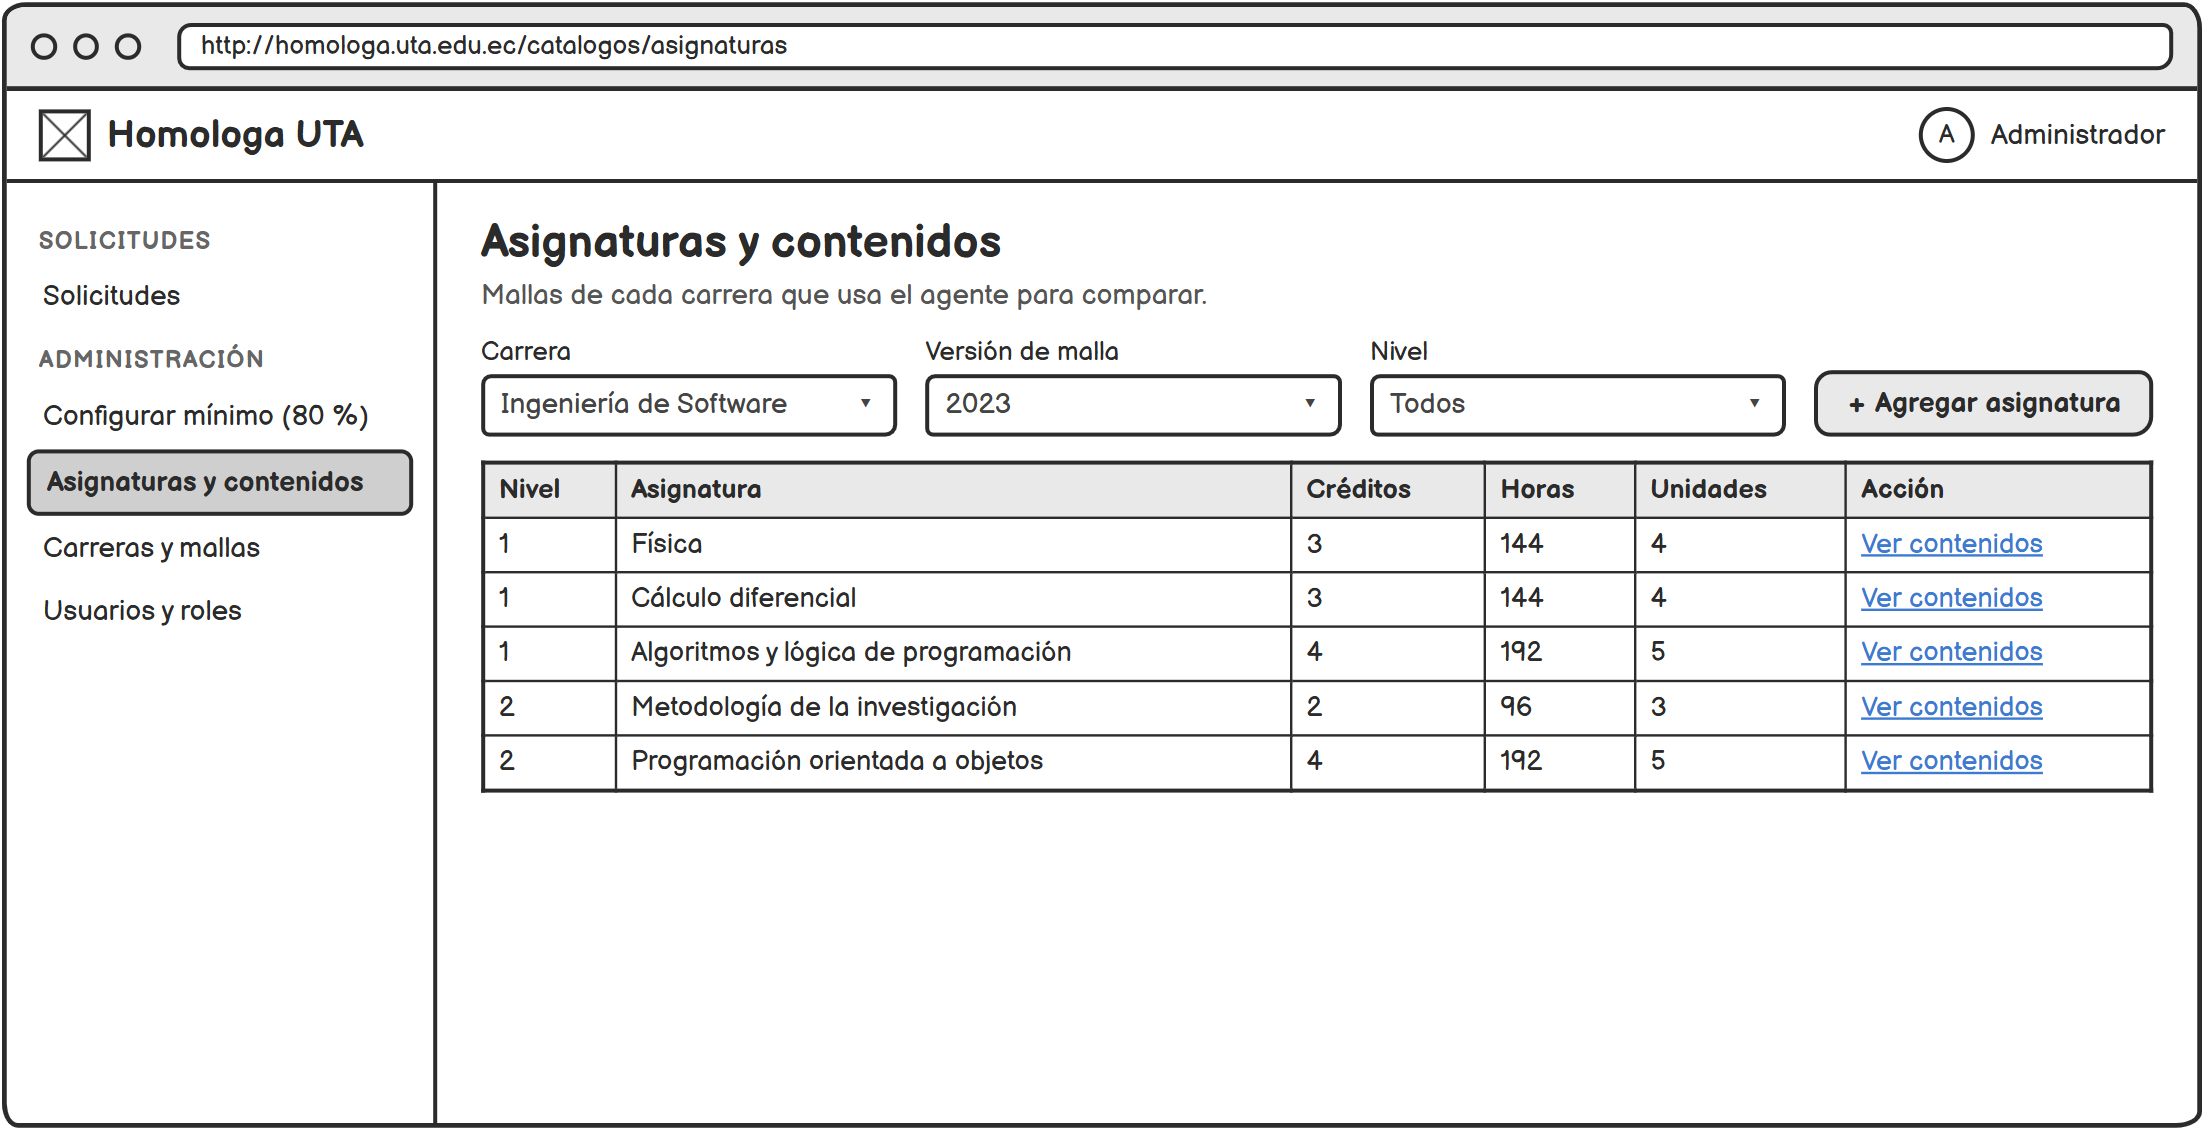
\includegraphics[width=0.93\textwidth]{mockups/m03.png}}
\caption{Mockup M-03 -- Asignaturas de la malla}
\end{figure}
\par\needspace{6\baselineskip}\noindent\textbf{\textit{Pruebas de aceptación -- HU-03}}\par
\begin{longtable}{|p{1.4cm}|p{3.7cm}|p{4.6cm}|p{5.1cm}|}
\hline\rowcolor{grisTarjeta}\textbf{N.º} & \textbf{Prueba} & \textbf{Entrada} & \textbf{Resultado esperado}\\\hline
\endhead
PA-03.1 & Carreras y versiones de malla & El administrador abre Carreras y mallas. & Listado de carreras y versiones\\\hline
PA-03.2 & Asignaturas con créditos, horas y unidades & El administrador abre Asignaturas y contenidos. & Créditos, horas y unidades\\\hline
\caption{Pruebas de aceptación de la HU-03}
\end{longtable}

\subsubsection{HU-04: API Gateway}
\historia{HU-04}{Responsable de arquitectura}{Entrada central con permisos}{Alta}{Media}{5 SP}{Sprint 1}{Jair León; Alex Jonathan Chisag; Rolando Sebastián Miranda; Paul Acurio}{Como responsable de arquitectura, quiero centralizar las rutas y validar los permisos, para dirigir cada petición al servicio correspondiente.}{\item Dado un token válido y permisos adecuados, cuando se envía una petición, entonces llega al servicio previsto.\item Dado un token ausente o un rol sin permiso, cuando se accede a una ruta protegida, entonces el Gateway rechaza la petición.}{Historia habilitadora US-04.}{M-04 (Acceso denegado por rol)}
\casosdeuso{HU-04}{Usuario del sistema}{{Entrar por el Gateway},{Validar la sesión},{Comprobar el permiso\\por rol},{Mostrar acceso denegado}}{1}{\incluye{1}{2}\incluye{2}{3}\extiende{4}{3}}{Toda petición entra por el Gateway, que valida la sesión y el rol; si el rol no tiene permiso, se muestra acceso denegado.}
\par\needspace{8\baselineskip}\noindent\textbf{\textit{Desglose de tareas -- HU-04}}\par
La historia se divide en 5 tareas que suman 14,5 horas.\par\medskip
\tarea{S1-A01}{HU-04}{Preparación de proyecto React, cliente REST con interceptores JWT y mocks}{D}{2,9 h}{Día 1 del Sprint 1}{Día 1 del Sprint 1}{Alex Jonathan Chisag Punina}{Inicializar la SPA en React 18 + Vite + TypeScript, configurar el cliente HTTP centralizado apuntando al API Gateway con inyección de cabeceras Authorization: Bearer y preparar mocks para desarrollo paralelo.}
\tarea{S1-J06}{HU-04}{Configuración de enrutamiento Ocelot, validación JWT y políticas RBAC}{D}{2,9 h}{Día 6 del Sprint 1}{Día 6 del Sprint 1}{Jair Alexander León Tusa}{Configurar las rutas del API Gateway hacia los Microservicios A, B y C, activando la validación de firma de tokens JWT y las restricciones de acceso por rol en el borde.}
\tarea{S1-S07}{HU-04}{Pruebas de integración del API Gateway y conectividad del bus RabbitMQ}{C}{2,9 h}{Día 7 del Sprint 1}{Día 7 del Sprint 1}{Rolando Sebastián Miranda Baño}{Ejecutar pruebas automatizadas de acceso a través del API Gateway y verificar la conectividad del bus de eventos con dependencias aisladas y manejo de errores controlados.}
\tarea{S1-P08}{HU-04}{Auditoría de rutas del Gateway y respuestas HTTP 401, 403 y 404}{M}{2,9 h}{Día 8 del Sprint 1}{Día 8 del Sprint 1}{Paul Medardo Acurio López}{Probar exhaustivamente todas las rutas expuestas en el API Gateway verificando los estados HTTP 401, 403 y 404 según el rol autenticado y la disponibilidad del recurso.}
\tarea{S1-J10}{HU-04}{Corrección de hallazgos de integración y pruebas de humo del backend}{C}{2,9 h}{Día 10 del Sprint 1}{Día 10 del Sprint 1}{Jair Alexander León Tusa}{Corregir hallazgos derivados de la integración entre el API Gateway y los microservicios, ejecutar revisión técnica de código y correr pruebas de humo del Sprint 1.}
\par\needspace{14\baselineskip}\noindent\textbf{\textit{Mockup de HU-04}}\par
\begin{figure}[H]\centering\fbox{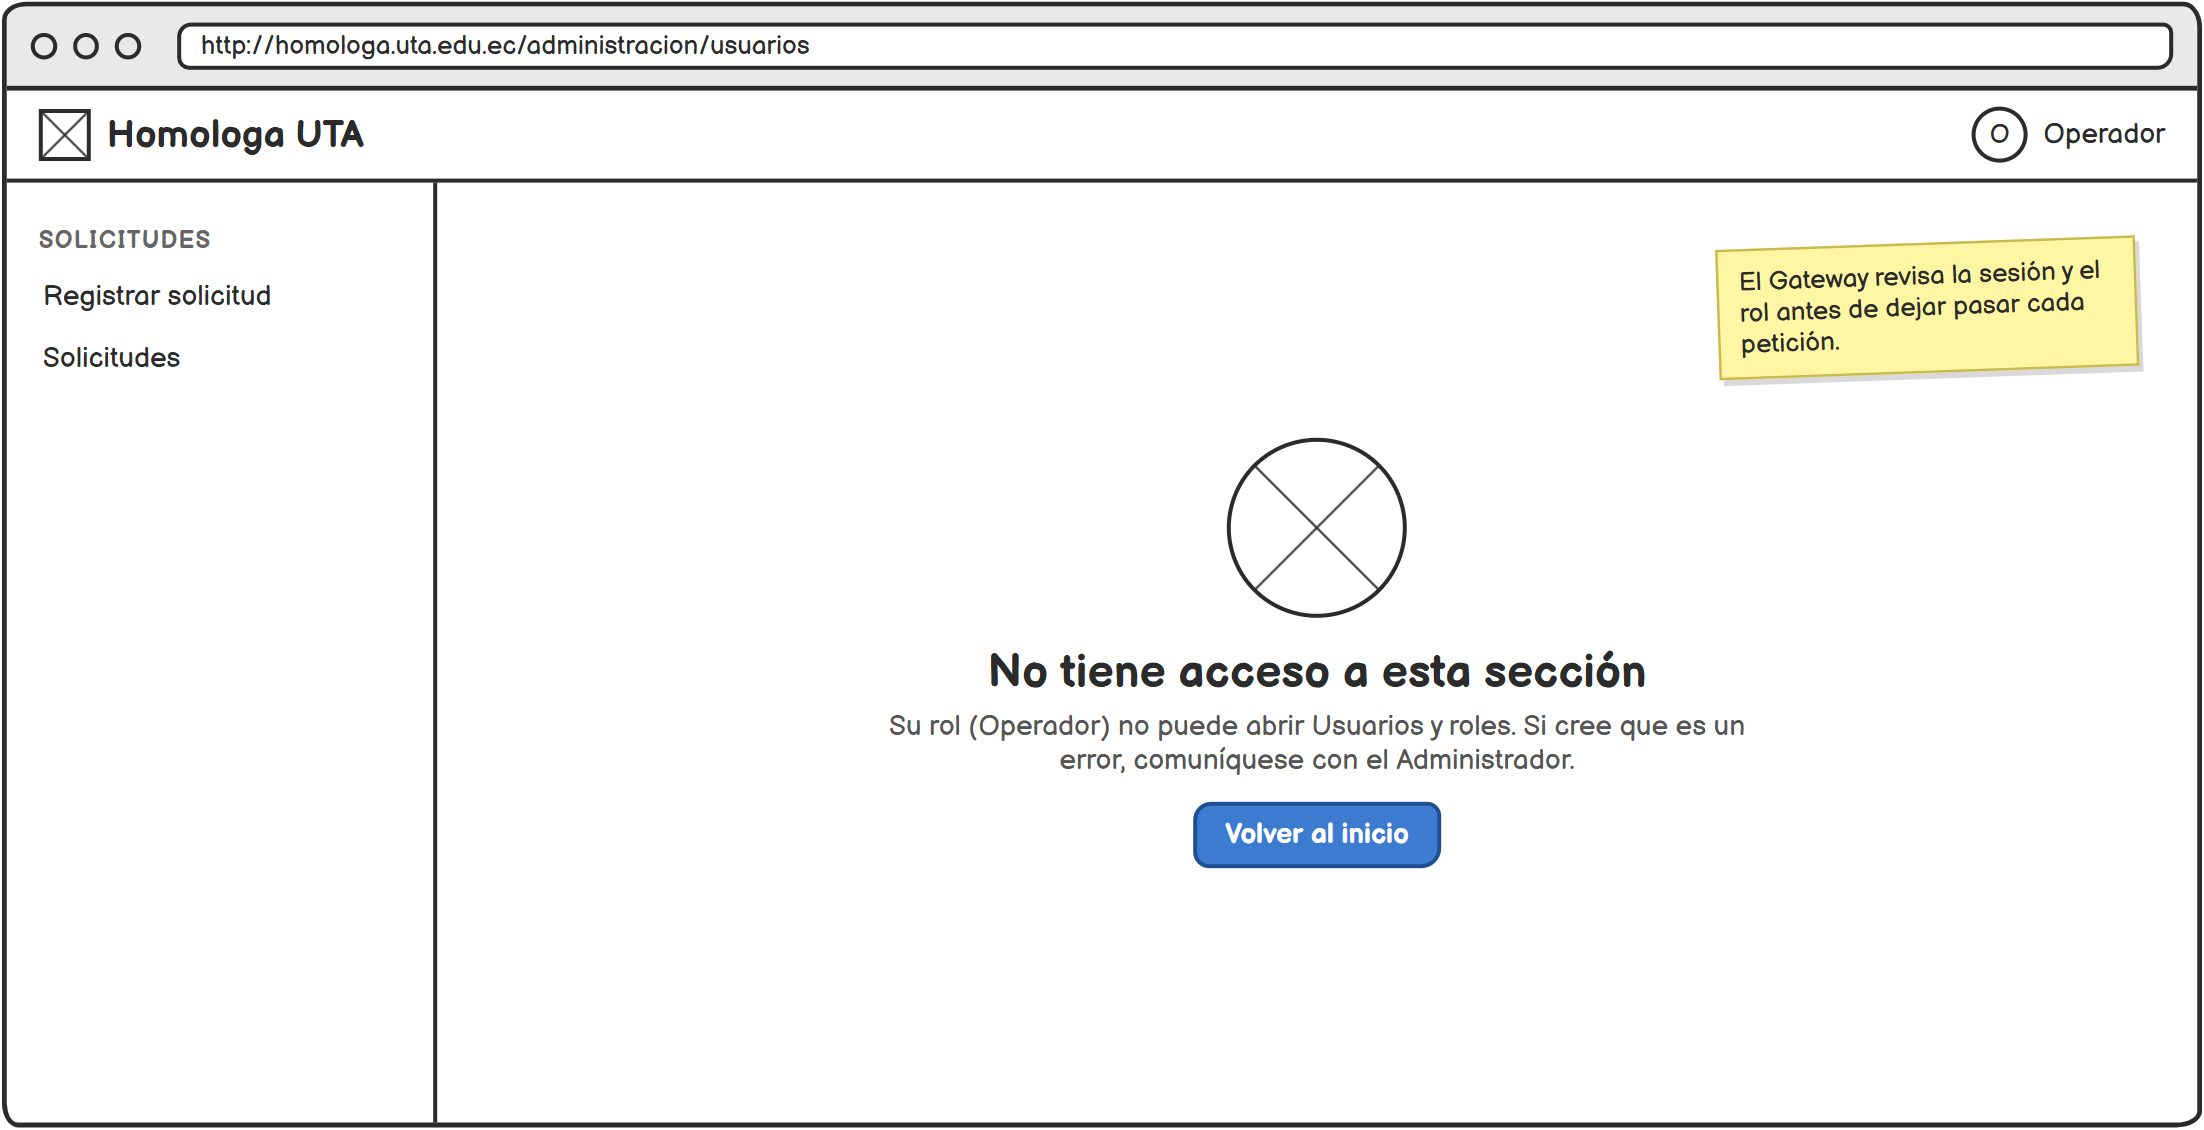
\includegraphics[width=0.93\textwidth]{mockups/m04.png}}
\caption{Mockup M-04 -- Acceso denegado por rol}
\end{figure}
\par\needspace{6\baselineskip}\noindent\textbf{\textit{Pruebas de aceptación -- HU-04}}\par
\begin{longtable}{|p{1.4cm}|p{3.7cm}|p{4.6cm}|p{5.1cm}|}
\hline\rowcolor{grisTarjeta}\textbf{N.º} & \textbf{Prueba} & \textbf{Entrada} & \textbf{Resultado esperado}\\\hline
\endhead
PA-04.1 & Petición sin iniciar sesión & Se pide la lista de usuarios al Gateway sin enviar el JWT. & 401 en el Gateway\\\hline
PA-04.2 & Un docente pide un recurso de administrador & Con la sesión del docente Carlos Paredes se pide la lista de usuarios. & 403 en el Gateway\\\hline
\caption{Pruebas de aceptación de la HU-04}
\end{longtable}

\subsubsection{HU-05: Expedientes y PDF}
\historia{HU-05}{Operador académico}{Registro de expedientes y documentos PDF}{Alta}{Media}{8 SP}{Sprint 1}{Rolando Sebastián Miranda; Alex Jonathan Chisag; Paul Acurio}{Como operador, quiero registrar expedientes internos o externos y adjuntar documentos PDF, para iniciar una solicitud de homologación.}{\item Dado un registro válido, cuando se envía, entonces se genera un identificador y se conserva su tipo de trámite.\item Dado un PDF inválido o información obligatoria ausente, cuando se carga, entonces se informa el error y no se acepta el expediente.}{Historia denominada US-05.}{M-05 (Registrar solicitud con sus PDF)}
\casosdeuso{HU-05}{Operador académico}{{Registrar expediente},{Adjuntar los PDF},{Validar formato y tamaño},{Consultar expedientes}}{1,2,4}{\incluye{2}{3}}{El operador registra el expediente y adjunta los PDF; cada archivo se valida antes de guardarse.}
\par\needspace{8\baselineskip}\noindent\textbf{\textit{Desglose de tareas -- HU-05}}\par
La historia se divide en 8 tareas que suman 23,2 horas.\par\medskip
\tarea{S1-S05}{HU-05}{Implementación de alta de solicitud interna/externa y validación de PDF en B}{D}{2,9 h}{Día 5 del Sprint 1}{Día 5 del Sprint 1}{Rolando Sebastián Miranda Baño}{Implementar en el Microservicio B la lógica de registro de solicitudes internas y externas, selección de materias del catálogo, fecha de aprobación certificada y validación de firma binaria, tamaño y formato de archivos PDF.}
\tarea{S1-S06}{HU-05}{Almacenamiento seguro de PDF y persistencia de metadatos en DB B}{D}{2,9 h}{Día 6 del Sprint 1}{Día 6 del Sprint 1}{Rolando Sebastián Miranda Baño}{Completar el guardado físico seguro de los archivos PDF y su asociación con la tabla EXPEDIENTE\_DOC en SQL Server DB B, habilitando el endpoint de consulta de metadatos y estado de recepción.}
\tarea{S1-A06}{HU-05}{Construcción del formulario web de nueva solicitud y carga de documentos PDF}{D}{2,9 h}{Día 6 del Sprint 1}{Día 6 del Sprint 1}{Alex Jonathan Chisag Punina}{Desarrollar en React 18 el formulario de registro de solicitudes (Interna / Externa), selector de institución de origen, carrera receptora, materias del catálogo y zona de carga de archivos PDF con validación local.}
\tarea{S1-P06}{HU-05}{Pruebas funcionales de alta de expedientes internos y externos}{M}{2,9 h}{Día 6 del Sprint 1}{Día 6 del Sprint 1}{Paul Medardo Acurio López}{Probar el registro de expedientes internos y externos verificando asignaturas seleccionadas, diferenciación de ruta normativa (CAU-P-011 / CAU-P-122) y rechazo ante ausencia de campos obligatorios.}
\tarea{S1-A07}{HU-05}{Integración del formulario de solicitud y carga multipart con Microservicio B}{D}{2,9 h}{Día 7 del Sprint 1}{Día 7 del Sprint 1}{Alex Jonathan Chisag Punina}{Conectar el formulario de registro y subida de archivos PDF con el endpoint real del Microservicio B a través del Gateway, mostrando en pantalla el identificador generado y los mensajes de error devueltos por la API.}
\tarea{S1-P07}{HU-05}{Pruebas de restricciones de archivos PDF (formato, tamaño y permisos)}{M}{2,9 h}{Día 7 del Sprint 1}{Día 7 del Sprint 1}{Paul Medardo Acurio López}{Ejecutar casos de prueba positivos y negativos sobre la carga de documentos: archivos que no son PDF, archivos que superan el tamaño límite, archivos vacíos y accesos con roles no autorizados.}
\tarea{S1-A09}{HU-05}{Verificación integrada de formularios, permisos y fallos de carga en UI}{C}{2,9 h}{Día 9 del Sprint 1}{Día 9 del Sprint 1}{Alex Jonathan Chisag Punina}{Integrar y verificar el comportamiento de los formularios de expedientes internos y externos ante fallos de carga o errores de validación del servidor, registrando los casos de aceptación de la interfaz.}
\tarea{S1-A10}{HU-05}{Revisión de usabilidad, navegación por teclado y preparación de demostración}{M}{2,9 h}{Día 10 del Sprint 1}{Día 10 del Sprint 1}{Alex Jonathan Chisag Punina}{Revisar la accesibilidad por teclado, consistencia de mensajes de validación y preparar la demostración reproducible del flujo del Sprint 1 en la interfaz web.}
\par\needspace{14\baselineskip}\noindent\textbf{\textit{Mockup de HU-05}}\par
\begin{figure}[H]\centering\fbox{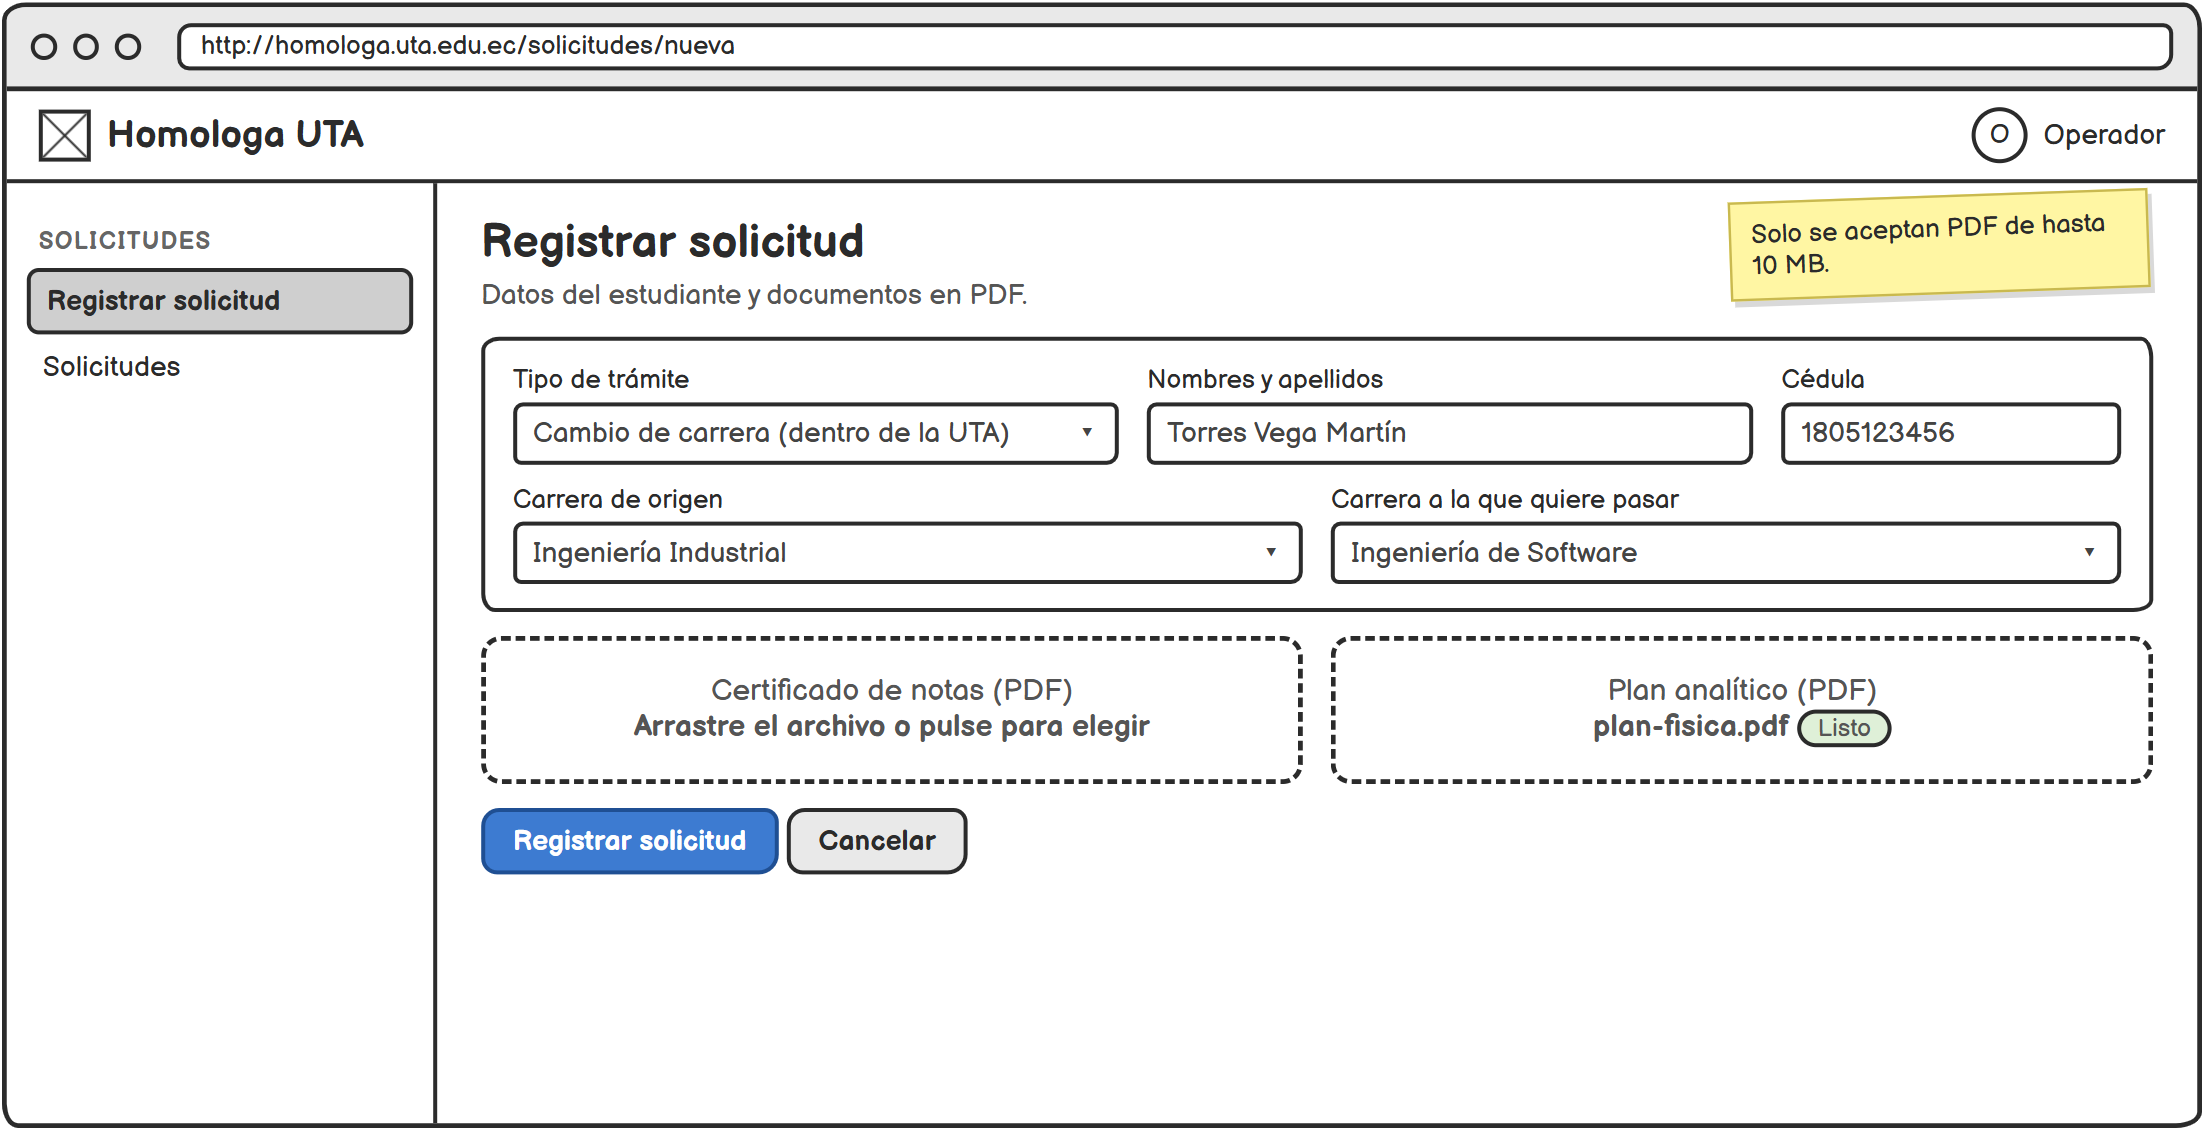
\includegraphics[width=0.93\textwidth]{mockups/m05.png}}
\caption{Mockup M-05 -- Registrar solicitud con sus PDF}
\end{figure}
\par\needspace{6\baselineskip}\noindent\textbf{\textit{Pruebas de aceptación -- HU-05}}\par
\begin{longtable}{|p{1.4cm}|p{3.7cm}|p{4.6cm}|p{5.1cm}|}
\hline\rowcolor{grisTarjeta}\textbf{N.º} & \textbf{Prueba} & \textbf{Entrada} & \textbf{Resultado esperado}\\\hline
\endhead
PA-05.1 & Archivo que no es el certificado & El operador sube un plan analítico suelto (E19) en lugar del certificado. & Rechazado; botón deshabilitado\\\hline
PA-05.2 & Registro de un certificado válido & El operador sube el certificado V05 y lo registra. & Expediente creado y enviado\\\hline
\caption{Pruebas de aceptación de la HU-05}
\end{longtable}

\subsubsection{HU-06: Publicación de solicitudes}
\historia{HU-06}{Responsable de integración}{Publicación de solicitudes en RabbitMQ}{Alta}{Media}{5 SP}{Sprint 1}{Paul Acurio; Rolando Sebastián Miranda}{Como responsable de integración, quiero publicar las solicitudes registradas en RabbitMQ, para que los servicios consumidores puedan procesarlas.}{\item Dado un expediente guardado, cuando se confirma su registro, entonces se publica un evento de solicitud creada.\item Dado que el bus no responde, cuando se intenta publicar, entonces se conserva la posibilidad de reintentar la publicación.}{Historia habilitadora denominada US-06.}{M-06 (Solicitud enviada al análisis)}
\casosdeuso{HU-06}{Operador académico}{{Registrar expediente},{Publicar el aviso\\de solicitud creada},{Recibir el aviso\\una sola vez}}{1}{\incluye{1}{2}\munieco{ana}{(11.2,-3.1)}{Servicio de\\Análisis}\draw (ana-w) -- (c3.east);}{Registrar un expediente incluye publicar el aviso en la cola; el Servicio de Análisis lo recibe una sola vez.}
\par\needspace{8\baselineskip}\noindent\textbf{\textit{Desglose de tareas -- HU-06}}\par
La historia se divide en 10 tareas que suman 29,0 horas.\par\medskip
\tarea{S1-P01}{HU-06}{Definición del contrato SolicitudCreadaEvent e identificador de correlación}{D}{2,9 h}{Día 1 del Sprint 1}{Día 1 del Sprint 1}{Paul Medardo Acurio López}{Definir formalmente la estructura del evento SolicitudCreadaEvent, el identificador de correlación (CorrelationId) y los metadatos mínimos requeridos para el intercambio asíncrono entre B y C.}
\tarea{S1-P04}{HU-06}{Pruebas de publicación en RabbitMQ mediante suscriptor de prueba}{M}{2,9 h}{Día 4 del Sprint 1}{Día 4 del Sprint 1}{Paul Medardo Acurio López}{Implementar y ejecutar un suscriptor de prueba en RabbitMQ para verificar que el mensaje publicado cumpla exactamente el contrato acordado sin activar aún el análisis del Microservicio C.}
\tarea{S1-J07}{HU-06}{Configuración de MassTransit en B y publicación de SolicitudCreadaEvent}{D}{2,9 h}{Día 7 del Sprint 1}{Día 7 del Sprint 1}{Jair Alexander León Tusa}{Configurar el bus MassTransit con RabbitMQ en el Microservicio B e implementar la publicación del evento SolicitudCreadaEvent tras el registro válido de un expediente.}
\tarea{S1-J08}{HU-06}{Vinculación de persistencia con publicación y manejo de reintentos}{D}{2,9 h}{Día 8 del Sprint 1}{Día 8 del Sprint 1}{Jair Alexander León Tusa}{Conectar la persistencia del expediente en DB B con el publicador del bus, configurando políticas de reintento y registro de fallos sin perder la trazabilidad del identificador.}
\tarea{S1-S08}{HU-06}{Configuración de pipeline de Integración Continua (CI) y pruebas automatizadas}{O}{2,9 h}{Día 8 del Sprint 1}{Día 8 del Sprint 1}{Rolando Sebastián Miranda Baño}{Configurar el pipeline de integración continua para compilar automáticamente los microservicios, ejecutar la suite de pruebas xUnit y generar el reporte de resultados en cada cambio.}
\tarea{S1-J09}{HU-06}{Integración de Gateway, expediente y publicador del bus con trazabilidad}{D}{2,9 h}{Día 9 del Sprint 1}{Día 9 del Sprint 1}{Jair Alexander León Tusa}{Integrar el recorrido completo del Sprint 1 desde el API Gateway hasta la persistencia en DB B y la publicación en RabbitMQ, verificando la respuesta HTTP 202 Accepted .}
\tarea{S1-P09}{HU-06}{Verificación de correlación del evento y recuperación ante fallos del bus}{M}{2,9 h}{Día 9 del Sprint 1}{Día 9 del Sprint 1}{Paul Medardo Acurio López}{Ejecutar pruebas de fallo y recuperación desconectando temporalmente RabbitMQ para comprobar que el publicador reintenta el envío conservando el identificador de correlación.}
\tarea{S1-S09}{HU-06}{Ejecución de pruebas integradas de reglas, expedientes, PDF y evento}{C}{2,9 h}{Día 9 del Sprint 1}{Día 9 del Sprint 1}{Rolando Sebastián Miranda Baño}{Ejecutar pruebas integradas de extremo a extremo sobre el flujo de recepción de solicitudes, carga de PDF y publicación del evento en el bus, corrigiendo los defectos detectados.}
\tarea{S1-P10}{HU-06}{Ejecución de regresión funcional completa del flujo US-01 a US-06}{M}{2,9 h}{Día 10 del Sprint 1}{Día 10 del Sprint 1}{Paul Medardo Acurio López}{Ejecutar la batería de regresión funcional de las seis historias del Sprint 1 ( US-01 a US-06) y consolidar las evidencias reproducibles para la revisión del incremento.}
\tarea{S1-S10}{HU-06}{Arranque limpio en Docker Compose, consolidación de QA y guía de ejecución}{O}{2,9 h}{Día 10 del Sprint 1}{Día 10 del Sprint 1}{Rolando Sebastián Miranda Baño}{Verificar el levantamiento desde cero de todos los contenedores en Docker Compose, consolidar el reporte de calidad y documentar la guía reproducible de ejecución del Sprint 1.}
\par\needspace{14\baselineskip}\noindent\textbf{\textit{Mockup de HU-06}}\par
\begin{figure}[H]\centering\fbox{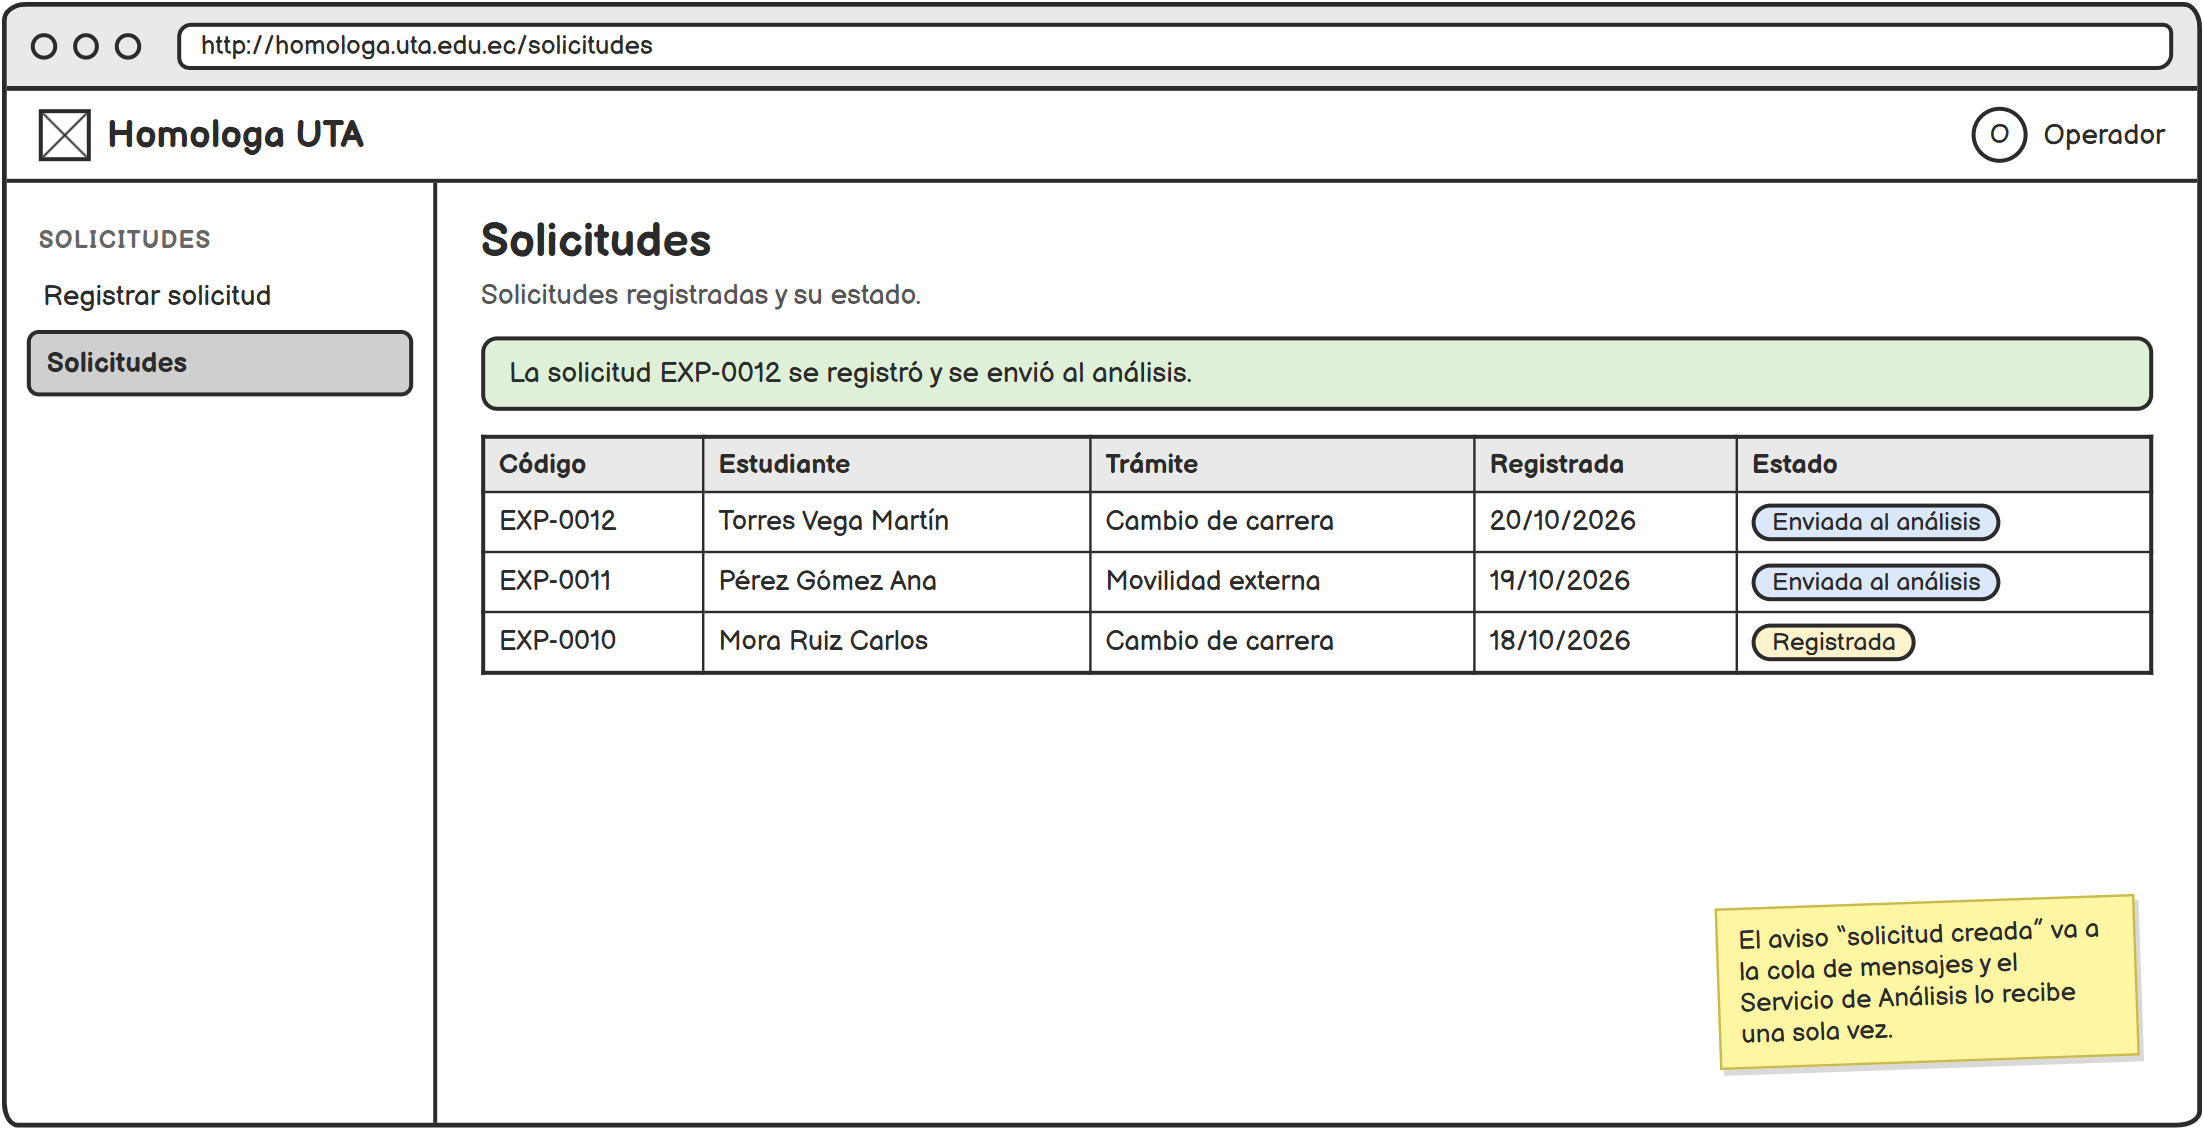
\includegraphics[width=0.93\textwidth]{mockups/m06.png}}
\caption{Mockup M-06 -- Solicitud enviada al análisis}
\end{figure}
\par\needspace{6\baselineskip}\noindent\textbf{\textit{Pruebas de aceptación -- HU-06}}\par
\begin{longtable}{|p{1.4cm}|p{3.7cm}|p{4.6cm}|p{5.1cm}|}
\hline\rowcolor{grisTarjeta}\textbf{N.º} & \textbf{Prueba} & \textbf{Entrada} & \textbf{Resultado esperado}\\\hline
\endhead
PA-06.1 & Publicación del evento en RabbitMQ & Después de registrar, se consultan las colas de RabbitMQ y el registro del Microservicio C. & Evento publicado y procesado\\\hline
\caption{Pruebas de aceptación de la HU-06}
\end{longtable}

\subsection{Incremento entregado y retrospectiva}
El informe del Sprint 2 señala como punto de partida que el Sprint 1 dejó usuarios y roles, reglas configurables, catálogo de carreras, entrada por Gateway y registro de solicitudes con sus PDF. La retrospectiva orientó mejoras en coordinación, integración y verificación continua; los hallazgos pendientes alimentaron el trabajo del Sprint 2.

\section{Sprint 2: análisis de la solicitud}
\subsection{Propósito y objetivos}
El propósito fue procesar planes con texto o escaneados, calcular créditos y contenidos con las reglas vigentes y consultar precedentes para entregar una estimación explicable a revisión docente. El período planificado fue del 21 de octubre al 4 de noviembre de 2026, con revisión el 4 de noviembre. Las cinco historias fueron HU-07 a HU-11.

\subsection{Capacidad}
\begin{tabularx}{\textwidth}{|X|l|c|c|c|c|}\hline\rowcolor{grisTarjeta}\textbf{Integrante} & \textbf{Rol} & \textbf{Brutas} & \textbf{Coordinación} & \textbf{Técnicas} & \textbf{Planificado}\\\hline
Jair León & Scrum Master / Backend & 30 h & 1 h & 29 h & 46 h\\\hline Paul Acurio & Product Owner Proxy / IA & 30 h & 1 h & 29 h & 36 h\\\hline Alex Chisag & Frontend / UI-UX & 30 h & 1 h & 29 h & 32 h\\\hline Rolando Sebastián Miranda & Backend / QA-DevOps & 30 h & 1 h & 29 h & 39 h\\\hline Total & & 120 h & 4 h & 116 h & 153 h\\\hline
\end{tabularx}\captionof{table}{Capacidad del Sprint 2}
Las tareas sumaron 153 horas frente a una capacidad técnica de 116 horas. La planificación registró una diferencia de 37 horas como riesgo del sprint.

\subsection{Sprint Backlog}
\begin{tabularx}{\textwidth}{|c|X|c|c|}\hline\rowcolor{grisTarjeta}\textbf{Historia} & \textbf{Alcance} & \textbf{SP} & \textbf{Horas}\\\hline
HU-07 & Leer el plan analítico y confirmar datos dudosos & 8 & 36\\\hline HU-08 & Calcular con reglas y umbrales aprobados & 3 & 18\\\hline HU-09 & Mostrar proporción de créditos y alertas & 3 & 20\\\hline HU-10 & Leer planes escaneados y comparar contenidos & 8 & 40\\\hline HU-11 & Consultar casos anteriores y resoluciones & 5 & 39\\\hline Total & & 27 & 153\\\hline
\end{tabularx}\captionof{table}{Sprint Backlog del Sprint 2}

\subsection{Historias y pruebas de aceptación}
Las siguientes tarjetas condensan las historias incluidas en el informe entregado del Sprint 2. En la tabla de pruebas se resumen los escenarios de aceptación descritos en sus secciones.

\subsubsection{HU-07: Lectura del plan y confirmación}
\historia{HU-07}{Operador académico}{Leer el plan analítico y confirmar los datos dudosos}{Alta}{Media}{8 SP}{21 al 23 de octubre}{Jair León (5 h); Paul Acurio (8 h); Alex Chisag (13 h); Rolando Miranda (10 h)}{Como operador académico, quiero que el sistema lea créditos, horas y temas del PDF y me pida revisar lo que no leyó con seguridad, para evitar evaluar con datos equivocados.}{\item Dado un PDF con texto, cuando se envía, entonces se muestran los datos leídos y un aviso repetido no genera una evaluación duplicada.\item Dado un dato obligatorio ausente o confianza menor a 0,80, cuando termina la lectura, entonces queda pendiente de confirmación y no empieza el cálculo.\item Dado un PDF escaneado, cuando se procesa, entonces queda pendiente de lectura con IA y no se inventan datos.}{La lectura escaneada continúa en HU-10.}{M-01 y M-02}
\begin{longtable}{|p{1.45cm}|p{5.5cm}|p{1.9cm}|p{2.9cm}|p{0.95cm}|p{2.0cm}|}
\hline\rowcolor{grisTarjeta}\textbf{Número} & \textbf{Tarea} & \textbf{Tipo} & \textbf{Responsable} & \textbf{Horas} & \textbf{Fechas}\\\hline
\endhead
TA-07.1 & Recibir cada solicitud enviada una sola vez & Desarrollo & Jair León & 3 h & 21/10\\\hline
TA-07.2 & Preparar la IA local y las tablas del análisis & Otra & Sebastián Miranda & 5 h & 21/10\\\hline
TA-07.3 & Leer créditos, horas y unidades de un PDF con texto & Desarrollo & Paul Acurio & 5 h & 21/10\\\hline
TA-07.4 & Pantalla de bandeja de procesamiento & Desarrollo & Alex Chisag & 3 h & 21/10\\\hline
TA-07.5 & Servicios para consultar y confirmar los datos leídos & Desarrollo & Jair León & 2 h & 22/10\\\hline
TA-07.6 & Detectar PDF escaneados y lecturas poco seguras & Desarrollo & Paul Acurio & 3 h & 22/10\\\hline
TA-07.7 & Formulario para revisar y corregir los datos leídos & Desarrollo & Alex Chisag & 5 h & 22/10\\\hline
TA-07.8 & Pruebas unitarias de la lectura y del aviso repetido & Otra & Sebastián Miranda & 5 h & 22/10\\\hline
TA-07.9 & Conectar la confirmación con el Servicio de Análisis & Desarrollo & Alex Chisag & 5 h & 23/10\\\hline
\multicolumn{4}{|r|}{\textbf{Total}} & \textbf{36 h} & \\\hline
\caption{Tareas de la HU-07 (9 tareas)}
\end{longtable}

\begin{longtable}{|p{1.4cm}|p{3.7cm}|p{4.6cm}|p{5.1cm}|}
\hline\rowcolor{grisTarjeta}\textbf{N.º} & \textbf{Prueba} & \textbf{Entrada} & \textbf{Resultado esperado}\\\hline
\endhead
PA-07.1 & Lectura de un PDF con texto & Solicitud enviada con un plan analítico con texto & Se muestran los datos leídos con confianza 0,94 y el estado Datos leídos.\\\hline
PA-07.2 & Aviso de solicitud repetido & El mismo aviso llega dos veces & Se crea una sola evaluación.\\\hline
PA-07.3 & Lectura poco segura & PDF sin créditos legibles & Estado Confirmación pendiente; el cálculo no empieza.\\\hline
PA-07.4 & Confirmar con datos vacíos & Formulario con los créditos vacíos & Aviso Ingrese los créditos; no se guarda nada.\\\hline
PA-07.5 & PDF escaneado & PDF sin texto & Estado Pendiente de lectura con IA, sin datos inventados.\\\hline
\caption{Pruebas de aceptación de la HU-07 (definidas en el Sprint 2)}
\end{longtable}


\subsubsection{HU-08: Reglas y umbrales}
\historia{HU-08}{Docente evaluador}{Calcular con las reglas y umbrales aprobados}{Alta}{Media}{3 SP}{23 y 30 de octubre}{Jair León (10 h); Paul Acurio (3 h); Alex Chisag (2 h); Rolando Miranda (3 h)}{Como docente evaluador, quiero que el cálculo use las reglas vigentes aprobadas, para que el análisis sea consistente y explicable.}{\item Dada una solicitud confirmada, cuando se procesa, entonces el servicio consulta la versión vigente de las reglas.\item Dado un resultado calculado, cuando se presenta, entonces se identifican las reglas aplicadas.}{Consume las reglas del MS A.}{Reglas aplicadas en el análisis}
\begin{longtable}{|p{1.45cm}|p{5.5cm}|p{1.9cm}|p{2.9cm}|p{0.95cm}|p{2.0cm}|}
\hline\rowcolor{grisTarjeta}\textbf{Número} & \textbf{Tarea} & \textbf{Tipo} & \textbf{Responsable} & \textbf{Horas} & \textbf{Fechas}\\\hline
\endhead
TA-08.1 & Consultar las reglas vigentes al Servicio de Reglas & Desarrollo & Jair León & 10 h & 23/10\\\hline
TA-08.2 & Probar el cambio de un umbral y la caída del servicio & Mejora & Paul Acurio & 3 h & 23/10\\\hline
TA-08.3 & Pruebas de integración de la consulta de reglas & Otra & Sebastián Miranda & 3 h & 23/10\\\hline
TA-08.4 & Mostrar en las pantallas las reglas aplicadas & Desarrollo & Alex Chisag & 2 h & 30/10\\\hline
\multicolumn{4}{|r|}{\textbf{Total}} & \textbf{18 h} & \\\hline
\caption{Tareas de la HU-08 (4 tareas)}
\end{longtable}

\begin{longtable}{|p{1.4cm}|p{3.7cm}|p{4.6cm}|p{5.1cm}|}
\hline\rowcolor{grisTarjeta}\textbf{N.º} & \textbf{Prueba} & \textbf{Entrada} & \textbf{Resultado esperado}\\\hline
\endhead
PA-08.1 & Reglas en el resultado & Reglas en su versión 3; análisis de un expediente & El resultado muestra 80 ~\%, 15 ~\%, 0,75 y versión 3.\\\hline
PA-08.2 & Cambio de umbral & El administrador sube el parecido mínimo a 0,80 & Se usa 0,80 y la versión sube a 4.\\\hline
PA-08.3 & Servicio de Reglas apagado & Análisis de un expediente confirmado & Estado Pendiente de reglas con el error registrado.\\\hline
\caption{Pruebas de aceptación de la HU-08 (definidas en el Sprint 2)}
\end{longtable}


\subsubsection{HU-09: Créditos y alertas}
\historia{HU-09}{Docente evaluador}{Ver proporción de créditos y alertas}{Alta}{Media}{3 SP}{26 de octubre}{Jair León (7 h); Paul Acurio (5 h); Alex Chisag (3 h); Rolando Miranda (5 h)}{Como docente evaluador, quiero ver la proporción de créditos y las alertas antes de comparar, para valorar las condiciones de la solicitud.}{\item Dado un caso con créditos, cuando se analiza, entonces se muestra su proporción.\item Dado un caso fuera de las condiciones de vigencia o matrícula, cuando se analiza, entonces se presentan las alertas.}{Depende de los datos confirmados de HU-07 y las reglas de HU-08.}{Resumen de créditos y alertas}
\begin{longtable}{|p{1.45cm}|p{5.5cm}|p{1.9cm}|p{2.9cm}|p{0.95cm}|p{2.0cm}|}
\hline\rowcolor{grisTarjeta}\textbf{Número} & \textbf{Tarea} & \textbf{Tipo} & \textbf{Responsable} & \textbf{Horas} & \textbf{Fechas}\\\hline
\endhead
TA-09.1 & Calcular la proporción de créditos y los controles de vigencia y matrícula & Desarrollo & Jair León & 7 h & 26/10\\\hline
TA-09.2 & Pruebas de los controles con casos de la normativa & Mejora & Paul Acurio & 5 h & 26/10\\\hline
TA-09.3 & Panel de créditos y alertas & Desarrollo & Alex Chisag & 3 h & 26/10\\\hline
TA-09.4 & Pruebas con casos límite del cálculo de créditos & Otra & Sebastián Miranda & 5 h & 26/10\\\hline
\multicolumn{4}{|r|}{\textbf{Total}} & \textbf{20 h} & \\\hline
\caption{Tareas de la HU-09 (4 tareas)}
\end{longtable}

\begin{longtable}{|p{1.4cm}|p{3.7cm}|p{4.6cm}|p{5.1cm}|}
\hline\rowcolor{grisTarjeta}\textbf{N.º} & \textbf{Prueba} & \textbf{Entrada} & \textbf{Resultado esperado}\\\hline
\endhead
PA-09.1 & Créditos suficientes & 4 créditos de origen y 3 de destino & 100,00 ~\% con la etiqueta dato de apoyo.\\\hline
PA-09.2 & Créditos insuficientes & 2 créditos de origen y 3 de destino & 66,67 ~\%.\\\hline
PA-09.3 & Destino sin créditos & 4 frente a 0 & Mensaje de error; no se calcula.\\\hline
PA-09.4 & Materia de más de 10 años & Cambio de carrera; materia aprobada hace 12 años & Alerta de vigencia y paso a Validación de conocimientos.\\\hline
PA-09.5 & Tercera matrícula & Estudiante con tercera matrícula & Caso bloqueado con la alerta correspondiente.\\\hline
\caption{Pruebas de aceptación de la HU-09 (definidas en el Sprint 2)}
\end{longtable}


\subsubsection{HU-10: Lectura escaneada y comparación}
\historia{HU-10}{Docente evaluador}{Leer planes escaneados y comparar tema por tema}{Alta}{Alta}{8 SP}{27 al 29 de octubre}{Jair León (11 h); Paul Acurio (13 h); Alex Chisag (5 h); Rolando Miranda (11 h)}{Como docente evaluador, quiero que el sistema lea planes escaneados y compare sus temas, para revisar la cobertura de contenidos con evidencia.}{\item Dado un PDF escaneado, cuando se procesa, entonces se extrae información sin inventar los campos que no se reconocen.\item Dadas las materias de origen y destino, cuando se comparan, entonces se presenta el resultado por tema.}{Usa datos confirmados y reglas vigentes.}{Comparación de contenidos}
\begin{longtable}{|p{1.45cm}|p{5.5cm}|p{1.9cm}|p{2.9cm}|p{0.95cm}|p{2.0cm}|}
\hline\rowcolor{grisTarjeta}\textbf{Número} & \textbf{Tarea} & \textbf{Tipo} & \textbf{Responsable} & \textbf{Horas} & \textbf{Fechas}\\\hline
\endhead
TA-10.1 & Representar los temas con la IA local & Desarrollo & Jair León & 3 h & 27/10\\\hline
TA-10.2 & Leer PDF escaneados con OCR e IA sin inventar datos & Desarrollo & Paul Acurio & 4 h & 27/10\\\hline
TA-10.3 & Pantalla del estado de la lectura & Desarrollo & Alex Chisag & 2 h & 27/10\\\hline
TA-10.4 & Guardar los vectores de las materias de Software & Desarrollo & Sebastián Miranda & 3 h & 27/10\\\hline
TA-10.5 & Comparar temas y calcular el porcentaje de contenido & Desarrollo & Jair León & 4 h & 28/10\\\hline
TA-10.6 & Ajustar la comparación con casos reales & Mejora & Paul Acurio & 4 h & 28/10\\\hline
TA-10.7 & Tabla de cobertura por unidad & Desarrollo & Alex Chisag & 3 h & 28/10\\\hline
TA-10.8 & Pruebas unitarias del porcentaje de contenido & Otra & Sebastián Miranda & 5 h & 28/10\\\hline
TA-10.9 & Combinar dos materias de origen para un destino & Desarrollo & Jair León & 4 h & 29/10\\\hline
TA-10.10 & Pruebas funcionales de la combinación y de los temas faltantes & Mejora & Paul Acurio & 5 h & 29/10\\\hline
TA-10.11 & Pruebas de carga de la lectura con IA & Otra & Sebastián Miranda & 3 h & 29/10\\\hline
\multicolumn{4}{|r|}{\textbf{Total}} & \textbf{40 h} & \\\hline
\caption{Tareas de la HU-10 (11 tareas)}
\end{longtable}

\begin{longtable}{|p{1.4cm}|p{3.7cm}|p{4.6cm}|p{5.1cm}|}
\hline\rowcolor{grisTarjeta}\textbf{N.º} & \textbf{Prueba} & \textbf{Entrada} & \textbf{Resultado esperado}\\\hline
\endhead
PA-10.1 & PDF escaneado legible & PDF sin texto & Datos leídos; lo dudoso queda vacío para el operador.\\\hline
PA-10.2 & Cobertura de 6 de 7 unidades & 7 unidades de 12 h; 6 con parecido de 0,75 o más & 85,71 ~\% y la unidad 7 marcada como faltante.\\\hline
PA-10.3 & Parecido bajo el umbral & Unidad con parecido 0,74 & La unidad queda como faltante.\\\hline
PA-10.4 & Dos materias para un destino & Física I y Física II para Física & Los temas se suman sin contarse dos veces.\\\hline
PA-10.5 & Misma materia en dos destinos & Física I usada en dos destinos & El sistema lo rechaza.\\\hline
\caption{Pruebas de aceptación de la HU-10 (definidas en el Sprint 2)}
\end{longtable}


\subsubsection{HU-11: Precedentes}
\historia{HU-11}{Docente evaluador}{Consultar casos anteriores y sus resoluciones}{Media}{Media}{5 SP}{29 de octubre al 3 de noviembre}{Jair León (13 h); Paul Acurio (7 h); Alex Chisag (9 h); Rolando Miranda (10 h)}{Como docente evaluador, quiero consultar casos anteriores idénticos y su resolución, para disponer de antecedentes durante la revisión.}{\item Dada una solicitud con materias identificables, cuando se consulta, entonces se muestran precedentes coincidentes y su resolución.\item Dado que no hay precedentes, cuando se consulta, entonces se informa que no existen coincidencias.}{La búsqueda de casos anteriores aporta contexto para la revisión.}{Consulta de precedentes}
\begin{longtable}{|p{1.45cm}|p{5.5cm}|p{1.9cm}|p{2.9cm}|p{0.95cm}|p{2.0cm}|}
\hline\rowcolor{grisTarjeta}\textbf{Número} & \textbf{Tarea} & \textbf{Tipo} & \textbf{Responsable} & \textbf{Horas} & \textbf{Fechas}\\\hline
\endhead
TA-11.1 & Pantalla de consulta de precedentes & Desarrollo & Alex Chisag & 5 h & 29/10\\\hline
TA-11.2 & Guardar precedentes y buscarlos por coincidencia exacta & Desarrollo & Jair León & 8 h & 30/10\\\hline
TA-11.3 & Cargar resoluciones anteriores de prueba & Mejora & Paul Acurio & 3 h & 30/10\\\hline
TA-11.4 & Pruebas de la búsqueda de precedentes & Otra & Sebastián Miranda & 5 h & 30/10\\\hline
TA-11.5 & Unir todos los pasos del análisis & Desarrollo & Jair León & 3 h & 02/11\\\hline
TA-11.6 & Verificar que un precedente no salte los controles & Mejora & Paul Acurio & 2 h & 02/11\\\hline
TA-11.7 & Mensajes de error claros en la interfaz & Corrección & Alex Chisag & 2 h & 02/11\\\hline
TA-11.8 & Prueba completa del flujo entre servicios & Otra & Sebastián Miranda & 3 h & 02/11\\\hline
TA-11.9 & Ordenar el código y cerrar la parte técnica & Mejora & Jair León & 2 h & 03/11\\\hline
TA-11.10 & Repetir las pruebas funcionales y guardar evidencias & Mejora & Paul Acurio & 2 h & 03/11\\\hline
TA-11.11 & Revisar el aspecto de las pantallas y preparar la demostración & Mejora & Alex Chisag & 2 h & 03/11\\\hline
TA-11.12 & Agregar las pruebas a la integración continua & Otra & Sebastián Miranda & 2 h & 03/11\\\hline
\multicolumn{4}{|r|}{\textbf{Total}} & \textbf{39 h} & \\\hline
\caption{Tareas de la HU-11 (12 tareas)}
\end{longtable}

\begin{longtable}{|p{1.4cm}|p{3.7cm}|p{4.6cm}|p{5.1cm}|}
\hline\rowcolor{grisTarjeta}\textbf{N.º} & \textbf{Prueba} & \textbf{Entrada} & \textbf{Resultado esperado}\\\hline
\endhead
PA-11.1 & Coincidencia exacta & Física I y Física II para Física, misma universidad & Se muestran la resolución, las materias y la universidad.\\\hline
PA-11.2 & Sin coincidencia & Bases de Datos I, Universidad de Cuenca & Aviso Sin precedentes registrados.\\\hline
PA-11.3 & Caso solo parecido & Física I sola para Física & No se muestra como coincidencia.\\\hline
PA-11.4 & Precedente y más de 10 años & Precedente favorable; materia de hace 12 años & Igual pide validación de conocimientos y revisión docente.\\\hline
PA-11.5 & Falla la búsqueda & Servicio de precedentes sin respuesta & Aviso; los cálculos de créditos y temas continúan.\\\hline
\caption{Pruebas de aceptación de la HU-11 (definidas en el Sprint 2)}
\end{longtable}


\subsection{Resultado del Sprint 2}
El informe del Sprint 2 registra la demostración del incremento con lectura, confirmación de datos, reglas, créditos, contenidos y precedentes. Una prueba de aceptación de HU-11 (PA-11.5) quedó pendiente y otra quedó parcial según la evidencia de ejecución. En el trabajo posterior se abordó la falla del servicio y el reintento automático, descritos en la sección de correcciones.

\section{Correcciones del Sprint 2}\label{sec:correcciones}
Después de revisar el incremento y aclarar el flujo esperado, se realizaron ajustes funcionales y de calidad. Las referencias de commits se conservan para identificar los cambios del repositorio.

\subsection{C-01: Certificado SIHA único}
El flujo anterior consideraba un plan analítico suelto y una bandeja para revisar su lectura OCR. Se cambió porque Secretaría emite un certificado SIHA único que concentra la documentación del trámite. Se adaptó la recepción para usar ese certificado como documento de entrada; la prueba PA-10.1 queda reemplazada por el escenario correspondiente al certificado SIHA. Commits: \texttt{55d6ac3}, \texttt{c8abebd}, \texttt{687f6bf}, \texttt{f1b71d6}. La verificación es la recepción y validación del certificado único por el flujo actualizado.

\subsection{C-02: Regla de créditos y contenidos}
La interpretación anterior combinaba un mínimo de 80~\% de contenido con una tolerancia de créditos. Tras la aclaración con el docente, los créditos por debajo del 80~\% bloquean el caso y no permiten votación; los contenidos por debajo del 80~\% se presentan como recomendación y la decisión corresponde a los docentes. Se actualizaron la regla y su presentación para distinguir ambos criterios. Commits: \texttt{35d0796}, \texttt{6aa9054}, \texttt{03eb265}, \texttt{cc3812d}. La prueba se comprueba con casos de créditos inferiores al umbral y con cobertura de contenidos inferior al umbral, verificando bloqueo y recomendación respectivamente.

\subsection{C-03: Reintento ante servicio no disponible}
Algunas pruebas pendientes no definían un estado claro cuando el servicio de análisis no respondía. Se agregó el estado ``El agente se está preparando'' y el reintento automático. Commits: \texttt{fc4cae5}, \texttt{28c495d}. La corrección cubre PA-08.3 y PA-11.5: al no responder el servicio, el estado se informa y el procesamiento se reintenta.

\subsection{C-04: Calidad técnica}
Se corrigió el redondeo de valores decimales, se estabilizó la prueba del bus, se incorporó ESLint, se ajustó el tratamiento de PDF como binarios en Git y se actualizaron pruebas de integración. Commits: \texttt{9602631}, \texttt{3b863e5}, \texttt{1d359be}. La comprobación se realiza con las pruebas del bus y de integración, la revisión del formato decimal y la validación estática del frontend.

\subsection{C-05: Interfaz y mensajes}
Se reorganizó el menú lateral; los errores aparecen junto al botón relacionado; se corrigió el botón que quedaba cubierto por el menú; el acceso denegado se expresa en lenguaje sencillo; y se añadieron opciones para confirmar y restablecer la contraseña. Commit: \texttt{0a3f102}. La comprobación consiste en recorrer las pantallas afectadas y verificar la visibilidad de controles y mensajes.

\subsection{C-06: Solicitudes con el formato anterior}
Las solicitudes recibidas con el formato anterior deben conservarse como registros históricos, pero sus números de certificado pueden volver a utilizarse en el flujo actualizado. Se liberan esos números sin borrar las solicitudes. Commit: \texttt{28c495d}. La comprobación verifica que el número vuelva a estar disponible y que el expediente histórico permanezca registrado.

\begin{tabularx}{\textwidth}{|c|X|X|X|}\hline
\rowcolor{grisTarjeta}\textbf{Código} & \textbf{Corrección} & \textbf{Commits} & \textbf{Verificación}\\\hline
C-01 & Certificado SIHA único y reemplazo de PA-10.1 & \texttt{55d6ac3}, \texttt{c8abebd}, \texttt{687f6bf}, \texttt{f1b71d6} & Recepción y validación del certificado\\\hline
C-02 & Bloqueo por créditos y recomendación por contenidos & \texttt{35d0796}, \texttt{6aa9054}, \texttt{03eb265}, \texttt{cc3812d} & Casos bajo el 80~\%\\\hline
C-03 & Estado de preparación y reintento automático & \texttt{fc4cae5}, \texttt{28c495d} & PA-08.3 y PA-11.5\\\hline
C-04 & Redondeo, bus, ESLint, PDF y pruebas de integración & \texttt{9602631}, \texttt{3b863e5}, \texttt{1d359be} & Pruebas técnicas y revisión estática\\\hline
C-05 & Ajustes de menú, errores, acceso y contraseña & \texttt{0a3f102} & Recorrido de pantallas\\\hline
C-06 & Liberación de números del formato anterior & \texttt{28c495d} & Número disponible e historial conservado\\\hline
\end{tabularx}
\captionof{table}{Resumen de correcciones del Sprint 2}

\section{Planificación del Sprint 3}

\subsection{Descripción y fechas}
El Sprint 3 se desarrolló del 4 al 25 de noviembre de 2026. El equipo completó el flujo desde el registro de un certificado SIHA hasta el análisis, la revisión de los docentes y la decisión final cuando no hay acuerdo.

\subsection{Propósito y objetivos}
El propósito fue entregar una homologación explicable y revisable, con datos oficiales de la UTA y atención a los trámites externos. Se planificó registrar y revisar certificados, analizar las materias con el agente, aclarar el uso del mínimo del 80~\%, permitir los votos docentes y la decisión administrativa, guardar resultados por materia e incorporar registro manual y mejoras de cuentas.

\subsection{Análisis de capacidad}
Las horas de la tabla son la suma de las estimaciones de las tareas de código identificadas en los commits del período. No incluyen actividades sin un commit que las respalde.

\begin{table}[H]\centering\small
\begin{tabularx}{\textwidth}{|X|X|c|}\hline
\rowcolor{grisTarjeta}\textbf{Integrante} & \textbf{Rol en el sprint} & \textbf{Horas de tareas}\\\hline
Alex Jonathan Chisag & Frontend e integración & 57 h\\\hline
Rolando Sebastián Miranda & Backend, integración y pruebas & 58 h\\\hline
Jair León & Backend y correcciones & 15 h\\\hline
Paul Acurio & sin tareas de código registradas en el Sprint 3 & 0 h\\\hline
\textbf{Total registrado} & & \textbf{130 h}\\\hline
\end{tabularx}\caption{Capacidad de trabajo registrada en el Sprint 3}
\end{table}

\subsection{Product Backlog actualizado}
Las historias HU-01 a HU-06 del Sprint 1 están terminadas. Las HU-07 a HU-11 del Sprint 2 están terminadas con las correcciones descritas en la sección 7. El Sprint 3 tomó las historias HU-12 a HU-19, enfocadas en el certificado SIHA, el análisis, las decisiones y la operación del sistema.

\subsection{Sprint Backlog}
\begin{table}[H]\centering\small
\begin{tabularx}{\textwidth}{|c|X|X|c|c|c|}\hline
\rowcolor{grisTarjeta}\textbf{HU} & \textbf{Historia} & \textbf{Responsables con commits} & \textbf{SP} & \textbf{Horas} & \textbf{Prioridad}\\\hline
HU-12 & Registrar solicitud con certificado único y revisar antes del envío & Alex Jonathan Chisag; Jair León; Rolando Sebastián Miranda & 8 & 43 & Alta\\\hline
HU-13 & Analizar con sílabos oficiales y explicar cada materia & Rolando Sebastián Miranda; Alex Jonathan Chisag & 8 & 26 & Alta\\\hline
HU-14 & Comparar sílabo de otra universidad & Alex Jonathan Chisag & 5 & 4 & Media\\\hline
HU-15 & Aplicar la regla de créditos y contenidos del 80~\% & Alex Jonathan Chisag; Rolando Sebastián Miranda & 8 & 24 & Alta\\\hline
HU-16 & Registrar votos docentes y decisión final del administrador & Alex Jonathan Chisag; Rolando Sebastián Miranda & 8 & 14 & Alta\\\hline
HU-17 & Guardar el resultado de homologación por materia & Alex Jonathan Chisag & 5 & 4 & Media\\\hline
HU-18 & Registrar manualmente y sugerir solo materias relacionadas & Rolando Sebastián Miranda; Jair León & 5 & 11 & Media\\\hline
HU-19 & Administrar cuentas y avisar sobre la sesión & Alex Jonathan Chisag & 5 & 4 & Media\\\hline
\textbf{Total} & & & \textbf{52} & \textbf{130} & \\\hline
\end{tabularx}\caption{Sprint Backlog del Sprint 3}
\end{table}
Las horas del Sprint Backlog incluyen commits compartidos entre historias cuando el cambio atiende más de una necesidad; en la capacidad se cuentan una sola vez.

\subsection{Orden de elaboración y dependencias}
Primero se aseguró el ingreso y la revisión del certificado (HU-12), necesarios para crear solicitudes válidas. Luego se conectó el análisis a los sílabos y al reintento del agente (HU-13), además de la comparación externa (HU-14). La regla aclarada (HU-15) define qué materias bloquea el sistema y cuáles quedan para decisión docente. Sobre el análisis se construyeron los votos y la decisión final (HU-16), y el resultado consultable por materia (HU-17). El registro manual (HU-18) reutiliza la misma validación y análisis; las cuentas y sesión (HU-19) completan la operación por rol.

\subsection{Cronograma}
\begin{table}[H]\centering\small
\begin{tabularx}{\textwidth}{|c|X|X|}\hline
\rowcolor{grisTarjeta}\textbf{Semana} & \textbf{Trabajo principal} & \textbf{Historias y resultados}\\\hline
4 al 10 de noviembre & Certificado único, validación previa, mejoras de extracción y primer análisis con datos UTA & HU-12 y HU-13\\\hline
11 al 17 de noviembre & Tabla de resultados, movilidad externa y definición de la regla mínima & HU-14, HU-15 y HU-17\\\hline
18 al 25 de noviembre & Votos, decisión administrativa, registro manual, sesión y pruebas finales & HU-16, HU-18 y HU-19\\\hline
\end{tabularx}\caption{Cronograma de trabajo del Sprint 3}
\end{table}

\subsection{Burndown}
Para comparar el avance, se toma como trabajo inicial la suma de las estimaciones por commit de la sección 9. La línea real representa las horas pendientes al cierre de cada fecha que tuvo commits; la línea ideal baja de forma uniforme entre el 4 y el 25 de noviembre. Las estimaciones son una reconstrucción para el informe, no horas registradas en un control horario.

\begin{figure}[H]\centering
\begin{tikzpicture}
\begin{axis}[width=0.92\textwidth,height=7cm,xmin=4,xmax=25,ymin=0,ymax=135,xtick={4,10,13,14,22,24,25},xlabel={Día de noviembre de 2026},ylabel={Horas pendientes},grid=major,legend pos=north east]
\addplot[blue,dashed,thick] coordinates {(4,130)(25,0)};\addlegendentry{Ideal}
\addplot[red,mark=*,thick] coordinates {(4,130)(4.2,91)(13,61)(14,53)(22,45)(24,22)(25,0)};\addlegendentry{Real según commits}
\end{axis}
\end{tikzpicture}
\caption{Burndown reconstruido con las fechas de los commits del Sprint 3}
\end{figure}

\subsection{Riesgos y mitigación}
\begin{itemize}
\item El cambio de regla conversado con el docente podía afectar análisis y decisiones. Se separó el bloqueo por créditos de la recomendación por contenidos y se reflejó en pruebas y textos.
\item La IA local Ollama podía tardar o no estar disponible. Se añadió reintento automático y un estado comprensible para la solicitud.
\item El trabajo en ramas paralelas podía causar diferencias de integración. Se corrigieron contratos, migraciones y pruebas de integración antes del cierre.
\item Los datos de prueba podían no representar certificados reales. Se prepararon certificados SIHA de ejemplo, casos con errores y pruebas manuales por rol.
\end{itemize}

\subsection{Criterios de finalización}
El sprint se considera terminado cuando el certificado se valida antes de registrarse, el análisis presenta su recomendación por materia, los dos docentes pueden votar, un desacuerdo requiere decisión motivada del administrador, los resultados quedan disponibles por materia y el registro manual aplica controles equivalentes. También se consideran las pruebas automáticas, la ronda manual documentada en la sección 10 y los hallazgos pendientes explícitos.

\section{Historias de usuario: Sprint 3}

Las tareas se identifican con los commits de la fuente del sprint. Las horas son estimaciones razonables para el cambio descrito; la fecha de inicio y fin corresponde al día del commit. Los commits de Claude se asignan a Rolando Sebastián Miranda por su integración de los PR 17 y 18 y el merge indicado.

\subsection{HU-12: Registrar la solicitud con un único certificado SIHA y revisarlo antes de enviarlo}
\historia{HU-12}{Operador}{Registrar la solicitud con un único certificado SIHA y revisarlo antes de enviarlo}{Alta}{Alta}{8 SP}{4 al 13 de noviembre}{Alex Jonathan Chisag; Jair León; Rolando Sebastián Miranda}{Como operador, quiero registrar una solicitud con un certificado SIHA único y revisar los datos leídos antes de enviarla, para corregir problemas antes de que comience el análisis.}{\item Dado un certificado SIHA válido, cuando se registra, entonces queda una solicitud visible con sus datos y estado.\item Dado un certificado con campos incorrectos, cuando se revisa, entonces aparece una lista de verificación por sección y no se permite registrarlo.\item Dado un certificado ya registrado, cuando se intenta enviarlo otra vez, entonces se informa de la solicitud existente.}{El flujo utiliza el formato SIHA-CH-01 y evita duplicar el análisis.}{Registro y revisión del certificado}
\begin{figure}[H]\centering\begin{tikzpicture}[actor/.style={draw,ellipse},caso/.style={draw,ellipse,minimum width=3.3cm},node distance=1.1cm and 2cm]\node[actor] (a) {Operador};\node[caso,right=of a,yshift=1cm] (sube) {Subir certificado};\node[caso,below=of sube] (revisa) {Revisar secciones};\node[caso,below=of revisa] (registra) {Registrar solicitud};\draw (a)--(sube);\draw (a)--(revisa);\draw (a)--(registra);\draw[dashed] (revisa)--node[right]{«incluye»}(registra);\end{tikzpicture}\caption{Casos de uso de HU-12}\end{figure}
\textbf{Desglose de tareas}
\tarea{T12.1}{HU-12}{Registrar solicitud con certificado único}{D}{6 h}{4 nov. 2026}{4 nov. 2026}{Rolando Sebastián Miranda}{Commit 55d6ac3: se conectó el certificado único con el flujo de homologación automática por contenidos.}
\tarea{T12.2}{HU-12}{Validar certificado antes del registro}{D}{5 h}{13 nov. 2026}{13 nov. 2026}{Alex Jonathan Chisag}{Commit f1b71d6: se añadió la revisión previa del certificado antes de guardarlo.}
\tarea{T12.3}{HU-12}{Sugerir materia oficial de destino}{M}{3 h}{13 nov. 2026}{13 nov. 2026}{Alex Jonathan Chisag}{Commit b1fa62d: se sugirió el nombre oficial de la materia de destino.}
\tarea{T12.4}{HU-12}{Guardar contexto certificado y matrícula}{D}{4 h}{4 nov. 2026}{4 nov. 2026}{Jair León}{Commit 4c8a20e: se guardó el contexto de materias certificadas y matrícula.}
\tarea{T12.5}{HU-12}{Mejorar lectura OCR y revisión del operador}{C}{4 h}{4 nov. 2026}{4 nov. 2026}{Jair León}{Commit 9655d53: se reforzó la lectura OCR y el flujo para que el operador revise los datos.}
\tarea{T12.6}{HU-12}{Listar materias de la carrera elegida}{C}{3 h}{4 nov. 2026}{4 nov. 2026}{Jair León}{Commit ae66e47: se corrigió la lista de materias de origen según la carrera seleccionada.}
\tarea{T12.7}{HU-12}{Ajustar errores de integración del certificado}{C}{3 h}{4 nov. 2026}{4 nov. 2026}{Rolando Sebastián Miranda}{Commit 4256e9f: se corrigió el conteo de migraciones de DB B para que las pruebas de integración encontraran la estructura.}
\tarea{T12.8}{HU-12}{Preparar certificados de prueba}{O}{4 h}{4 nov. 2026}{4 nov. 2026}{Rolando Sebastián Miranda}{Commit a793d91: se prepararon 26 certificados SIHA de prueba, un generador y sus resultados.}
\tarea{T12.9}{HU-12}{Aclarar avisos y campos del certificado}{M}{3 h}{4 nov. 2026}{4 nov. 2026}{Rolando Sebastián Miranda}{Commit 5a8845d: se ajustaron notas con coma, el aviso de sílabo ausente, el formato anterior y la carga incremental de datos.}
\tarea{T12.10}{HU-12}{Mostrar menú y gestión de contraseñas}{M}{4 h}{22 nov. 2026}{22 nov. 2026}{Alex Jonathan Chisag}{Commit 0a3f102: se ordenó el menú lateral, los avisos y la gestión de contraseñas; también se corrigieron mensajes de errores del flujo.}
\tarea{T12.11}{HU-12}{Marcar documentos como archivos binarios}{C}{2 h}{13 nov. 2026}{13 nov. 2026}{Alex Jonathan Chisag}{Commit 3b863e5: se indicó a Git que los PDF y las imágenes deben tratarse como archivos binarios.}
\tarea{T12.12}{HU-12}{Preparar docentes de ejemplo}{O}{2 h}{24 nov. 2026}{24 nov. 2026}{Rolando Sebastián Miranda}{Commit e5fcff3: se agregaron docentes de ejemplo para poder probar el flujo de revisión.}
\textbf{Lo que queda funcionando}
\begin{itemize}\item El operador revisa los datos del certificado y la lista de problemas antes de registrar.\item Las solicitudes muestran sus materias y estado; el certificado duplicado se relaciona con el registro existente.\item La lectura identifica las materias de la carrera elegida y conserva su contexto.\end{itemize}
\textbf{Pruebas de aceptación}
\begin{table}[H]\centering\small\begin{tabularx}{\textwidth}{|l|X|X|X|}\hline\rowcolor{grisTarjeta}\textbf{PA} & \textbf{Prueba} & \textbf{Entrada} & \textbf{Resultado esperado}\\\hline PA-12.1 & Solicitud registrada & Certificado SIHA válido & La solicitud aparece con sus datos y estado.\\\hline PA-12.2 & Lista de verificación & Certificado con datos que incumplen reglas & Se muestran las secciones y motivos; no se registra.\\\hline PA-12.3 & Certificado repetido & Mismo certificado cargado otra vez & Se avisa y se ofrece la solicitud existente.\\\hline\end{tabularx}\caption{Pruebas de aceptación de HU-12}\end{table}

\subsection{HU-13: Analizar con los sílabos oficiales de la UTA y explicar cada materia}
\historia{HU-13}{Docente}{Analizar con sílabos oficiales de la UTA y explicar cada materia}{Alta}{Alta}{8 SP}{4 al 24 de noviembre}{Rolando Sebastián Miranda; Alex Jonathan Chisag}{Como docente, quiero que el agente compare cada materia con los sílabos oficiales y explique sus resultados, para revisar una recomendación comprensible y actualizada.}{\item Dada una solicitud con materias de la UTA, cuando termina el análisis, entonces se explica el resultado de cada materia con sus datos y regla aplicada.\item Dado que el agente aún se prepara o no estaba disponible, cuando el servicio vuelve, entonces la solicitud se analiza automáticamente.}{El agente recomienda y los docentes deciden, según la regla vigente.}{Análisis por materia}
\begin{figure}[H]\centering\begin{tikzpicture}[actor/.style={draw,ellipse},caso/.style={draw,ellipse,minimum width=3.4cm},node distance=1.1cm and 2cm]\node[actor](a){Docente};\node[caso,right=of a,yshift=0.6cm](ver){Ver análisis};\node[caso,below=of ver](detalle){Revisar explicación};\node[caso,below=of detalle](reintento){Reintentar análisis};\draw(a)--(ver);\draw(a)--(detalle);\draw(a)--(reintento);\draw[dashed](ver)--node[right]{«incluye»}(detalle);\end{tikzpicture}\caption{Casos de uso de HU-13}\end{figure}
\textbf{Desglose de tareas}
\tarea{T13.1}{HU-13}{Cargar sílabos oficiales y explicar análisis}{D}{6 h}{4 nov. 2026}{4 nov. 2026}{Rolando Sebastián Miranda}{Commit 687f6bf: se conectó el agente a los sílabos oficiales UTA y se presentó el análisis explicado y el historial del certificado.}
\tarea{T13.2}{HU-13}{Simplificar la solicitud y asignar revisores}{M}{6 h}{4 nov. 2026}{4 nov. 2026}{Rolando Sebastián Miranda}{Commit c8abebd: se incorporaron los dos revisores docentes, el análisis al subir el PDF y una aplicación más sencilla.}
\tarea{T13.3}{HU-13}{Reintentar el análisis al estar listo el agente}{D}{4 h}{13 nov. 2026}{13 nov. 2026}{Alex Jonathan Chisag}{Commit fc4cae5: se agregó el reintento automático mientras el agente se preparaba.}
\tarea{T13.4}{HU-13}{Volver a analizar con reglas vigentes}{C}{4 h}{24 nov. 2026}{24 nov. 2026}{Rolando Sebastián Miranda}{Commit 28c495d: se habilitó el nuevo análisis con reglas vigentes y se liberaron certificados del formato anterior.}
\tarea{T13.5}{HU-13}{Estabilizar pruebas de calidad e integración}{C}{4 h}{13 nov. 2026}{13 nov. 2026}{Alex Jonathan Chisag}{Commit 9602631: se corrigió el redondeo decimal y se estabilizaron pruebas del bus y ESLint.}
\tarea{T13.6}{HU-13}{Ajustar contrato y ejecución de integración}{C}{2 h}{14 nov. 2026}{14 nov. 2026}{Alex Jonathan Chisag}{Commit 1d359be: se ajustaron pruebas de integración al evento v1.2 y a .NET 8.}
\textbf{Lo que queda funcionando}
\begin{itemize}\item El análisis presenta la explicación y recomendación por materia con información oficial disponible.\item Si el agente no estaba listo, la solicitud puede continuar al volver el servicio.\item La decisión queda para los docentes de acuerdo con la regla vigente.\end{itemize}
\textbf{Pruebas de aceptación}
\begin{table}[H]\centering\small\begin{tabularx}{\textwidth}{|l|X|X|X|}\hline\rowcolor{grisTarjeta}\textbf{PA} & \textbf{Prueba} & \textbf{Entrada} & \textbf{Resultado esperado}\\\hline PA-13.1 & Análisis explicado & Solicitud con materias UTA & Muestra explicación, regla y recomendación por materia.\\\hline PA-13.2 & Reintento automático & Agente vuelve a estar disponible & La solicitud continúa al análisis sin un nuevo registro.\\\hline\end{tabularx}\caption{Pruebas de aceptación de HU-13}\end{table}

\subsection{HU-14: Movilidad externa: comparar el sílabo de otra universidad}
\historia{HU-14}{Operador}{Comparar el sílabo de otra universidad}{Media}{Alta}{5 SP}{13 de noviembre}{Alex Jonathan Chisag}{Como operador, quiero adjuntar el sílabo de una materia aprobada en otra universidad, para que el agente pueda compararlo con el sílabo de destino de la UTA.}{\item Dada una solicitud de movilidad externa con sílabo válido, cuando se analiza, entonces el agente usa sus unidades y temas para comparar.\item Dada una materia sin sílabo externo, cuando se analiza, entonces se indica que no hay sílabo para comparar.}{El sílabo externo es opcional.}{Movilidad externa}
\begin{figure}[H]\centering\begin{tikzpicture}[actor/.style={draw,ellipse},caso/.style={draw,ellipse,minimum width=3.4cm},node distance=1.1cm and 2cm]\node[actor](a){Operador};\node[caso,right=of a,yshift=.6cm](adj){Adjuntar sílabo};\node[caso,below=of adj](anal){Analizar materia externa};\node[caso,below=of anal](ver){Ver comparación};\draw(a)--(adj);\draw(a)--(anal);\draw(a)--(ver);\draw[dashed](anal)--node[right]{«incluye»}(ver);\end{tikzpicture}\caption{Casos de uso de HU-14}\end{figure}
\textbf{Desglose de tareas}
\tarea{T14.1}{HU-14}{Comparar sílabo externo en movilidad}{D}{4 h}{13 nov. 2026}{13 nov. 2026}{Alex Jonathan Chisag}{Commit a9b5a8c: se incorporó la comparación del sílabo de otra universidad para movilidad externa.}
\textbf{Lo que queda funcionando}
\begin{itemize}\item El trámite externo acepta sílabos por materia y los usa en la comparación.\item Si no se adjunta uno, la materia queda para revisión docente sin comparación automática.\end{itemize}
\textbf{Pruebas de aceptación}
\begin{table}[H]\centering\small\begin{tabularx}{\textwidth}{|l|X|X|X|}\hline\rowcolor{grisTarjeta}\textbf{PA} & \textbf{Prueba} & \textbf{Entrada} & \textbf{Resultado esperado}\\\hline PA-14.1 & Comparación externa & Solicitud externa con sílabo & Compara unidades; sin documento informa que no hay sílabo para comparar.\\\hline\end{tabularx}\caption{Pruebas de aceptación de HU-14}\end{table}

\subsection{HU-15: Regla: créditos bajo 80~\% bloquean, contenidos bajo 80~\% solo recomiendan}
\historia{HU-15}{Docente}{Aplicar el mínimo de créditos y contenidos con efectos distintos}{Alta}{Alta}{8 SP}{14 al 25 de noviembre}{Alex Jonathan Chisag; Rolando Sebastián Miranda}{Como docente, quiero que los créditos bajo el mínimo bloqueen la homologación y que los contenidos bajos generen una recomendación, para aplicar la regla acordada con el docente.}{\item Dado que los créditos no llegan al 80~\%, cuando se analiza, entonces la materia queda bloqueada y no admite voto.\item Dado que solo los contenidos no llegan al 80~\%, cuando se analiza, entonces se recomienda no homologar y los docentes pueden decidir.}{La IA recomienda; los docentes conservan la decisión en los casos que no estén bloqueados por créditos.}{Aplicación de la regla del 80~\%}
\begin{figure}[H]\centering\begin{tikzpicture}[actor/.style={draw,ellipse},caso/.style={draw,ellipse,minimum width=3.4cm},node distance=1.1cm and 2cm]\node[actor](a){Docente};\node[caso,right=of a,yshift=.6cm](rev){Revisar porcentajes};\node[caso,below=of rev](bloq){Ver bloqueo por créditos};\node[caso,below=of bloq](rec){Ver recomendación por contenidos};\draw(a)--(rev);\draw(a)--(bloq);\draw(a)--(rec);\draw[dashed](rev)--node[right]{«extiende»}(bloq);\draw[dashed](rev)--node[right]{«extiende»}(rec);\end{tikzpicture}\caption{Casos de uso de HU-15}\end{figure}
\textbf{Desglose de tareas}
\tarea{T15.1}{HU-15}{Aplicar mínimos en la regla}{D}{6 h}{14 nov. 2026}{14 nov. 2026}{Alex Jonathan Chisag}{Commit 35d0796: se aplicó el mínimo del 80~\% en contenidos y créditos en la primera definición de la regla.}
\tarea{T15.2}{HU-15}{Separar recomendación y decisión docente}{M}{6 h}{24 nov. 2026}{24 nov. 2026}{Rolando Sebastián Miranda}{Commit 6aa9054: se dejó al agente recomendar y al docente decidir; también se incorporó el registro manual sin PDF.}
\tarea{T15.3}{HU-15}{Bloquear créditos insuficientes}{C}{4 h}{25 nov. 2026}{25 nov. 2026}{Alex Jonathan Chisag}{Commit 03eb265: se corrigió la regla para bloquear créditos bajos y dejar contenidos bajos como consejo.}
\tarea{T15.4}{HU-15}{Aclarar estados de recomendación}{C}{3 h}{25 nov. 2026}{25 nov. 2026}{Alex Jonathan Chisag}{Commit bcc90ec: se aclaró el resumen para distinguir las materias bloqueadas.}
\tarea{T15.5}{HU-15}{Corregir voto pendiente y créditos obligatorios}{C}{3 h}{25 nov. 2026}{25 nov. 2026}{Rolando Sebastián Miranda}{Commit cc3812d: se ajustó el aviso de decisión pendiente y el tratamiento de los créditos obligatorios.}
\tarea{T15.6}{HU-15}{Ajustar el texto de la regla en la base}{C}{2 h}{24 nov. 2026}{24 nov. 2026}{Rolando Sebastián Miranda}{Commit 17048b0: se corrigió el tamaño permitido para guardar la descripción de la regla RN-01.}
\textbf{Lo que queda funcionando}
\begin{itemize}\item Créditos por debajo del mínimo producen un bloqueo sin votación.\item Contenidos por debajo del mínimo producen una recomendación que los docentes pueden revisar y decidir.\item Profundidad y carga horaria se presentan como datos informativos.\end{itemize}
\textbf{Pruebas de aceptación}
\begin{table}[H]\centering\small\begin{tabularx}{\textwidth}{|l|X|X|X|}\hline\rowcolor{grisTarjeta}\textbf{PA} & \textbf{Prueba} & \textbf{Entrada} & \textbf{Resultado esperado}\\\hline PA-15.1 & Créditos inferiores al 80~\% & Materia con créditos insuficientes & Queda bloqueada y sin controles de voto.\\\hline PA-15.2 & Solo contenidos inferiores al 80~\% & Créditos suficientes y baja cobertura & Se muestra recomendación y se permiten los votos docentes.\\\hline\end{tabularx}\caption{Pruebas de aceptación de HU-15}\end{table}

\subsection{HU-16: Decisión de los dos docentes y decisión final del administrador cuando no coinciden}
\historia{HU-16}{Docentes y Administrador}{Registrar las dos decisiones docentes y resolver desacuerdos}{Alta}{Alta}{8 SP}{13 al 25 de noviembre}{Alex Jonathan Chisag; Rolando Sebastián Miranda}{Como docente revisor, quiero registrar mi voto por materia; como administrador, quiero resolver con un motivo los desacuerdos, para que cada solicitud alcance una decisión final trazable.}{\item Dada una materia revisable, cuando vota cada docente, entonces queda guardada su decisión.\item Dados votos distintos, cuando se presenta el resultado, entonces el administrador puede decidir y debe explicar el motivo.\item Dada una decisión final, cuando se intenta cambiar un voto, entonces el sistema lo impide.}{Los votos docentes se conservan como parte del expediente.}{Votos y decisión final}
\begin{figure}[H]\centering\begin{tikzpicture}[actor/.style={draw,ellipse},caso/.style={draw,ellipse,minimum width=3.6cm},node distance=1.1cm and 2.1cm]\node[actor](d){Docente};\node[actor,below=2.1cm of d](a){Administrador};\node[caso,right=of d](voto){Registrar voto};\node[caso,right=of a](final){Resolver desacuerdo};\node[caso,below=of voto](estado){Consultar resultado};\draw(d)--(voto);\draw(a)--(final);\draw(d)--(estado);\draw(a)--(estado);\draw[dashed](final)--node[right]{«extiende»}(estado);\end{tikzpicture}\caption{Casos de uso de HU-16}\end{figure}
\textbf{Desglose de tareas}
\tarea{T16.1}{HU-16}{Avisar sobre sesión y solicitudes docentes}{M}{4 h}{13 nov. 2026}{13 nov. 2026}{Alex Jonathan Chisag}{Commit 68a2e56: se agregó aviso de sesión próxima a vencer y aviso de nuevas solicitudes al docente.}
\tarea{T16.2}{HU-16}{Añadir decisión final del administrador}{D}{6 h}{24 nov. 2026}{24 nov. 2026}{Rolando Sebastián Miranda}{Commit 059c63a: se implementó la decisión final administrativa cuando los docentes no coinciden y el reenvío al agente.}
\tarea{T16.3}{HU-16}{Cerrar votos tras decisión final}{C}{4 h}{25 nov. 2026}{25 nov. 2026}{Alex Jonathan Chisag}{Commit 1d8798c: se cerraron los votos después de la decisión final y se aclaró el estado.}
\textbf{Lo que queda funcionando}
\begin{itemize}\item Cada docente registra su voto y el desacuerdo queda visible.\item El administrador resuelve el desacuerdo con un motivo.\item Una vez resuelto, los votos no pueden modificarse y la solicitud muestra su estado final.\end{itemize}
\textbf{Pruebas de aceptación}
\begin{table}[H]\centering\small\begin{tabularx}{\textwidth}{|l|X|X|X|}\hline\rowcolor{grisTarjeta}\textbf{PA} & \textbf{Prueba} & \textbf{Entrada} & \textbf{Resultado esperado}\\\hline PA-16.1 & Voto docente & Decisión del primer revisor & El voto queda guardado.\\\hline PA-16.2 & Sin acuerdo & Dos votos diferentes & La materia queda pendiente de decisión administrativa.\\\hline PA-16.3 & Decisión final con motivo & Decisión administrativa y motivo & Se guarda la decisión final y el motivo.\\\hline PA-16.4 & Votos cerrados & Intento de cambiar voto tras decisión & El sistema impide el cambio.\\\hline\end{tabularx}\caption{Pruebas de aceptación de HU-16}\end{table}

\subsection{HU-17: Tabla RESULTADO\_HOMOLOGACION con el resultado por materia}
\historia{HU-17}{Administrador}{Consultar el resultado de homologación por materia}{Media}{Media}{5 SP}{13 de noviembre}{Alex Jonathan Chisag}{Como administrador, quiero consultar una fila por materia con los porcentajes, la recomendación y el resultado final, para revisar los datos del proceso de forma ordenada.}{\item Dado un análisis terminado, cuando se consulta la tabla, entonces existe una fila por cada materia solicitada.\item Dada una decisión docente o administrativa, cuando cambia el resultado, entonces la fila refleja el resultado actualizado.}{La tabla complementa el análisis completo de la solicitud.}{Resultado por materia}
\begin{figure}[H]\centering\begin{tikzpicture}[actor/.style={draw,ellipse},caso/.style={draw,ellipse,minimum width=3.4cm},node distance=1.1cm and 2cm]\node[actor](a){Administrador};\node[caso,right=of a,yshift=.6cm](consulta){Consultar resultados};\node[caso,below=of consulta](detalle){Ver resultado por materia};\draw(a)--(consulta);\draw(a)--(detalle);\draw[dashed](consulta)--node[right]{«incluye»}(detalle);\end{tikzpicture}\caption{Casos de uso de HU-17}\end{figure}
\textbf{Desglose de tareas}
\tarea{T17.1}{HU-17}{Guardar resultados por materia}{D}{4 h}{13 nov. 2026}{13 nov. 2026}{Alex Jonathan Chisag}{Commit 5596b30: se creó la tabla RESULTADO\_HOMOLOGACION y se guardó el mínimo del reglamento en el resultado.}
\textbf{Lo que queda funcionando}
\begin{itemize}\item Hay una fila de resultado por materia, con la recomendación, los porcentajes y las decisiones.\item El resultado se actualiza conforme se completan las revisiones.\end{itemize}
\textbf{Pruebas de aceptación}
\begin{table}[H]\centering\small\begin{tabularx}{\textwidth}{|l|X|X|X|}\hline\rowcolor{grisTarjeta}\textbf{PA} & \textbf{Prueba} & \textbf{Entrada} & \textbf{Resultado esperado}\\\hline PA-17.1 & Resultado por materia & Análisis con varias materias & Existe una fila por materia con porcentajes, votos y resultado final.\\\hline\end{tabularx}\caption{Pruebas de aceptación de HU-17}\end{table}

\subsection{HU-18: Registro manual sin PDF, lo más automático posible y solo con materias que se relacionan}
\historia{HU-18}{Operador}{Registrar manualmente una solicitud y completar los datos posibles}{Media}{Alta}{5 SP}{24 al 25 de noviembre}{Rolando Sebastián Miranda; Jair León}{Como operador, quiero registrar los datos del certificado sin PDF y recibir sugerencias relacionadas, para atender casos en que no dispongo del archivo y reducir la escritura manual.}{\item Dada una carrera y un nivel, cuando se carga la malla, entonces se completa el historial con sus materias.\item Dada una materia aprobada sin relación con el destino, cuando se revisa la solicitud, entonces se muestra un aviso y no se registra esa relación.}{El registro manual utiliza controles equivalentes a los del certificado.}{Registro manual}
\begin{figure}[H]\centering\begin{tikzpicture}[actor/.style={draw,ellipse},caso/.style={draw,ellipse,minimum width=3.5cm},node distance=1.1cm and 2cm]\node[actor](a){Operador};\node[caso,right=of a,yshift=.6cm](datos){Ingresar datos};\node[caso,below=of datos](carga){Cargar materias de malla};\node[caso,below=of carga](valida){Validar relación de materias};\draw(a)--(datos);\draw(a)--(carga);\draw(a)--(valida);\draw[dashed](datos)--node[right]{«incluye»}(valida);\end{tikzpicture}\caption{Casos de uso de HU-18}\end{figure}
\textbf{Desglose de tareas}
\tarea{T18.1}{HU-18}{Mantener número revisado en registro manual}{C}{3 h}{24 nov. 2026}{24 nov. 2026}{Rolando Sebastián Miranda}{Commit 37bca1f: se corrigió para que el número revisado sea el mismo que queda registrado.}
\tarea{T18.2}{HU-18}{Completar registro manual y sugerencias relacionadas}{M}{4 h}{25 nov. 2026}{25 nov. 2026}{Rolando Sebastián Miranda}{Commit 28e15e5: se añadió el llenado automático y se limitaron las solicitudes a materias relacionadas.}
\tarea{T18.3}{HU-18}{Listas para nivel, materia por nivel y períodos de la UTA}{M}{4 h}{25 nov. 2026}{25 nov. 2026}{Jair León}{Commit ac93ec4: el nivel y la materia se eligen de listas (la materia se filtra por nivel) y los períodos académicos de la UTA vienen precargados.}
\textbf{Lo que queda funcionando}
\begin{itemize}\item Se puede ingresar una solicitud sin adjuntar el PDF y completar el historial desde la malla.\item Las sugerencias ayudan a seleccionar materias relacionadas y se informan las que no guardan relación.\end{itemize}
\textbf{Pruebas de aceptación}
\begin{table}[H]\centering\small\begin{tabularx}{\textwidth}{|l|X|X|X|}\hline\rowcolor{grisTarjeta}\textbf{PA} & \textbf{Prueba} & \textbf{Entrada} & \textbf{Resultado esperado}\\\hline PA-18.1 & Llenado automático & Carrera de origen y nivel & Se cargan materias de la malla y sus datos disponibles.\\\hline PA-18.2 & Materias no relacionadas & Materia de origen sin afinidad al destino & Se explica el problema y no se registra esa relación.\\\hline\end{tabularx}\caption{Pruebas de aceptación de HU-18}\end{table}

\subsection{HU-19: Cuentas y sesión: restablecer contraseña, aviso de sesión por vencer y solo entrar a páginas permitidas}
\historia{HU-19}{Administrador}{Administrar cuentas y proteger el acceso por rol}{Media}{Media}{5 SP}{13 al 22 de noviembre}{Alex Jonathan Chisag}{Como administrador, quiero restablecer contraseñas y como usuario quiero recibir un aviso de sesión próxima a vencer y volver solo a páginas permitidas, para operar con acceso controlado.}{\item Dada una cuenta, cuando el administrador restablece su contraseña, entonces puede definir una nueva.\item Dada una sesión próxima a vencer, cuando el usuario está activo, entonces recibe un aviso.\item Dado un destino no permitido para el rol, cuando inicia sesión, entonces el sistema lo redirige a una página autorizada.}{La autorización depende del rol asignado.}{Cuentas y sesión}
\begin{figure}[H]\centering\begin{tikzpicture}[actor/.style={draw,ellipse},caso/.style={draw,ellipse,minimum width=3.5cm},node distance=1.1cm and 2cm]\node[actor](a){Administrador};\node[actor,below=1.5cm of a](u){Usuario};\node[caso,right=of a](clave){Restablecer contraseña};\node[caso,right=of u](sesion){Avisar sesión próxima a vencer};\node[caso,below=of sesion](acceso){Validar página por rol};\draw(a)--(clave);\draw(u)--(sesion);\draw(u)--(acceso);\end{tikzpicture}\caption{Casos de uso de HU-19}\end{figure}
\textbf{Desglose de tareas}
\tarea{T19.1}{HU-19}{Gestionar contraseñas y avisos de sesión}{M}{4 h}{22 nov. 2026}{22 nov. 2026}{Alex Jonathan Chisag}{Commit 0a3f102: se incorporaron avisos claros, gestión de contraseñas y ajustes del menú.}
\textbf{Lo que queda funcionando}
\begin{itemize}\item El administrador dispone de la acción de restablecer contraseña.\item El usuario recibe un aviso de sesión próxima a vencer y el retorno tras iniciar sesión considera su rol.\end{itemize}
\textbf{Pruebas de aceptación}
\begin{table}[H]\centering\small\begin{tabularx}{\textwidth}{|l|X|X|X|}\hline\rowcolor{grisTarjeta}\textbf{PA} & \textbf{Prueba} & \textbf{Entrada} & \textbf{Resultado esperado}\\\hline PA-19.1 & Restablecer contraseña & Cuenta seleccionada por administrador & Permite definir una contraseña nueva.\\\hline PA-19.2 & Página permitida & Inicio de sesión con rol definido & Solo redirige a una ruta autorizada para ese rol.\\\hline\end{tabularx}\caption{Pruebas de aceptación de HU-19}\end{table}

\clearpage
\section{Resultados de las pruebas}

Las pruebas de aceptación de los tres sprints se volvieron a ejecutar el 25 de noviembre de 2026 sobre la versión final
del sistema (rama \texttt{develop}, commit \texttt{ac93ec4}) funcionando en el computador del equipo con Docker Compose:
interfaz web, API Gateway, los tres microservicios, RabbitMQ, SQL Server (una base por servicio) y Ollama. Cada rol
(Operador, dos Docentes revisores y Administrador) trabajó en una ventana de navegador separada, con su propia sesión.
Las capturas se tomaron directamente de la aplicación en ese momento y están en la carpeta \texttt{capturas}, con el
mismo orden y número de esta sección.

Como en el Sprint 2, las pruebas que no tienen pantalla se respaldan con la salida de la consola (RabbitMQ y SQL Server)
o con las pruebas automáticas del proyecto, que se ejecutan en la integración continua. Las pruebas del Sprint 1 y del
Sprint 2 cuya pantalla cambió por las correcciones de la sección~\ref{sec:correcciones} se ejecutaron sobre la pantalla
actual; cuando una prueba ya no aplica se indica la corrección que la reemplazó.

\textbf{Datos de prueba utilizados:} los certificados SIHA de la carpeta \texttt{documentos-prueba/certificados-pruebas}
(V02 a V07 válidos; E05, E06, E10, E18, E19 y E20 con errores), los sílabos oficiales de la UTA cargados en el
Microservicio A y los sílabos de la ESPOCH para la movilidad externa. Docentes revisores: Ing.~Carlos Paredes e Ing.~María Vaca.

% =====================================================================
\subsection{Sprint 1: base del sistema (HU-01 a HU-06)}

\subsubsection{HU-01 -- Gestionar cuentas y roles}

\prueba{PA-01.1: Lista de cuentas con su rol y estado}
{El administrador abre Usuarios y roles.}
{pa01-1-cuentas.png}{Cuentas registradas con su rol y estado (HU-01)}
{Se listan las cuentas institucionales con su rol (Administrador, Docente, Operador), su estado y su último acceso.
Cada fila ofrece Editar, Restablecer contraseña, Desactivar y Dar de baja.}{0.95}

\prueba{PA-01.2: Crear una cuenta con datos que no coinciden}
{El administrador intenta crear una cuenta escribiendo dos contraseñas distintas.}
{pa01-2-validacion.png}{Validación al crear una cuenta (HU-01)}
{El campo Confirmar contraseña se marca en rojo con el mensaje ``Las contraseñas no coinciden.'' y la cuenta no se crea.
El rol viene marcado como Operador por defecto, el de menos permisos.}{0.95}

\prueba{PA-01.3: Un rol sin permiso entra a Usuarios y roles}
{El operador escribe a mano la dirección de Usuarios y roles.}
{pa01-3-acceso-denegado.png}{Aviso de acceso para un rol sin permiso (HU-01)}
{El sistema muestra ``No tiene acceso a esta sección'' con el rol autorizado y el rol con el que entró, en lenguaje
sencillo y con los botones Ir al inicio y Cambiar de cuenta.}{0.95}

\subsubsection{HU-02 -- Configurar reglas y umbrales}

\prueba{PA-02.1: Reglas vigentes y catálogo normativo}
{El administrador abre Configurar mínimo (80~\%).}
{pa02-1-reglas.png}{Reglas y umbrales vigentes (HU-02)}
{Se muestra el contenido mínimo (80~\%) con su versión y el catálogo normativo. La regla RN-01 ya indica que los
créditos son obligatorios y que los contenidos solo generan una recomendación.}{0.80}

\prueba{PA-02.2: Intentar bajar el mínimo de 80~\%}
{El administrador escribe 70 en Contenido mínimo y guarda.}
{pa02-2-minimo.png}{El mínimo no se puede bajar de 80~\% (HU-02)}
{Aparece ``El contenido mínimo no puede ser menor que 80~\%: lo fija el reglamento de homologación de la UTA. Puede
exigir más, pero no menos.'' y no se guarda nada.}{0.95}

\subsubsection{HU-03 -- Gestionar carreras, mallas y asignaturas}

\prueba{PA-03.1: Carreras y versiones de malla}
{El administrador abre Carreras y mallas.}
{pa03-1-mallas.png}{Carreras de la FISEI y sus mallas (HU-03)}
{Se listan las carreras de la FISEI con sus versiones de malla, que son las que usa el agente para comparar.}{0.95}

\prueba{PA-03.2: Asignaturas con créditos, horas y unidades}
{El administrador abre Asignaturas y contenidos.}
{pa03-2-asignaturas.png}{Asignaturas y unidades temáticas (HU-03)}
{Cada asignatura muestra su nivel, créditos, horas y unidades temáticas cargadas desde los sílabos oficiales.}{0.95}

\subsubsection{HU-04 -- Entrada única por el API Gateway}

\prueba{PA-04.1: Petición sin iniciar sesión}
{Se pide la lista de usuarios al Gateway sin enviar el JWT.}
{pa04-1-401.png}{El Gateway rechaza la petición sin JWT (HU-04)}
{El Gateway responde \textbf{401 Unauthorized} y la petición no llega al Microservicio A.}{0.95}

\prueba{PA-04.2: Un docente pide un recurso de administrador}
{Con la sesión del docente Carlos Paredes se pide la lista de usuarios.}
{pa04-2-403.png}{El Gateway rechaza un rol sin permiso (HU-04)}
{El Gateway valida el JWT pero responde \textbf{403 Forbidden}, porque la gestión de cuentas es solo del Administrador.}{0.95}

\subsubsection{HU-05 -- Registrar solicitudes con su documento}

\prueba{PA-05.1: Archivo que no es el certificado}
{El operador sube un plan analítico suelto (E19) en lugar del certificado.}
{pa05-1-rechazo.png}{Rechazo de un documento que no es el certificado SIHA (HU-05)}
{Aparece ``Este PDF no es el certificado SIHA'' con el motivo, y el botón de registrar queda deshabilitado.}{0.95}

\prueba{PA-05.2: Registro de un certificado válido}
{El operador sube el certificado V05 y lo registra.}
{pa05-2-registro.png}{Solicitud registrada y enviada (HU-05)}
{Se crea el expediente con su código, se muestran el estudiante, el cambio de carrera, las materias pedidas y los
docentes revisores, y se indica que el agente ya está analizando.}{0.95}

\subsubsection{HU-06 -- Avisar a los otros servicios}

\prueba{PA-06.1: Publicación del evento en RabbitMQ}
{Después de registrar, se consultan las colas de RabbitMQ y el registro del Microservicio C.}
{pa06-1-rabbitmq.png}{Cola, intercambio del evento y procesamiento en MS C (HU-06)}
{Existe el intercambio \texttt{SolicitudCreadaEvent} y la cola \texttt{solicitud-creada-ms-c} con un consumidor y cero
mensajes pendientes. El registro de MS C muestra ``SolicitudCreadaEvent procesado'' para las solicitudes registradas.}{1.0}

\begin{table}[H]\centering\small
\begin{tabularx}{\textwidth}{|l|X|X|l|}\hline
\rowcolor{grisTarjeta}\textbf{N.º} & \textbf{Prueba} & \textbf{Resultado obtenido} & \textbf{Estado}\\\hline
PA-01.1 & Lista de cuentas & Cuentas con rol, estado y acciones & Cumple\\\hline
PA-01.2 & Datos que no coinciden & ``Las contraseñas no coinciden''; no se crea & Cumple\\\hline
PA-01.3 & Rol sin permiso & ``No tiene acceso a esta sección'' & Cumple\\\hline
PA-02.1 & Reglas vigentes & Mínimo 80~\% y catálogo RN & Cumple\\\hline
PA-02.2 & Bajar de 80~\% & Rechazado con mensaje claro & Cumple\\\hline
PA-03.1 & Carreras y mallas & Listado de carreras y versiones & Cumple\\\hline
PA-03.2 & Asignaturas & Créditos, horas y unidades & Cumple\\\hline
PA-04.1 & Sin JWT & 401 en el Gateway & Cumple\\\hline
PA-04.2 & Rol sin permiso & 403 en el Gateway & Cumple\\\hline
PA-05.1 & Documento equivocado & Rechazado; botón deshabilitado & Cumple\\\hline
PA-05.2 & Certificado válido & Expediente creado y enviado & Cumple\\\hline
PA-06.1 & Evento en RabbitMQ & Evento publicado y procesado & Cumple\\\hline
\end{tabularx}
\caption{Resultados de las pruebas del Sprint 1}
\end{table}

% =====================================================================
\clearpage
\subsection{Sprint 2: análisis de la solicitud (HU-07 a HU-11)}

Se repiten las 23 pruebas del documento del Sprint 2 con su mismo número. Desde la corrección C-01 el documento de
entrada es el certificado SIHA (ya no el plan analítico suelto), por eso las pruebas de lectura se ejecutan con él.

\subsubsection{HU-07 -- Leer el documento y confirmar los datos dudosos}

\prueba{PA-07.1: Lectura de un PDF con texto}
{El operador sube el certificado V05 (Industrial a Software).}
{pa07-1-datos-leidos.png}{Datos leídos del certificado (HU-07)}
{El sistema muestra el estudiante, el trámite, el certificado, los docentes revisores, las materias pedidas y el
historial académico completo con nivel, período, nota y estado.}{0.70}

\prueba{PA-07.2: Aviso de solicitud repetida}
{El operador vuelve a registrar el certificado V02, que ya estaba registrado.}
{pa07-2-repetido.png}{Aviso de certificado ya registrado (HU-07)}
{Junto al botón aparece ``El certificado SIHA-2026-0202 ya fue registrado en el expediente…'' con el enlace Ver la
solicitud registrada; no se crea una segunda solicitud. Que un mismo aviso de RabbitMQ no cree dos análisis lo
comprueba la prueba automática \texttt{Ignora\_evento\_duplicado\_sin\_crear\_otro\_registro}.}{0.95}

\prueba{PA-07.3: Lectura con datos que faltan}
{El operador sube el certificado E20, que tiene la cédula vacía y una materia sin período.}
{pa07-3-campos-vacios.png}{Certificado con campos sin llenar (HU-07)}
{La revisión muestra ``El certificado tiene campos sin llenar'', con la lista de verificación por sección y el botón
de registrar deshabilitado. El análisis no empieza.}{0.80}

\prueba{PA-07.4: Confirmar con datos vacíos}
{En el registro manual el operador pulsa Revisar los datos sin llenar el formulario.}
{pa07-4-manual-vacio.png}{Registro manual con datos vacíos (HU-07)}
{Se muestra la lista de lo que falta por sección y no se guarda nada.}{0.55}

\prueba{PA-07.5: PDF escaneado}
{El operador sube un PDF escaneado (E18).}
{pa07-5-escaneado.png}{PDF escaneado rechazado (HU-07)}
{Aparece ``Este PDF no es el certificado SIHA'' y se explica que el certificado debe generarse digitalmente; el
sistema no inventa datos.}{0.95}

\subsubsection{HU-08 -- Calcular con las reglas y umbrales aprobados}

\prueba{PA-08.1: Reglas en el resultado}
{Se abre el análisis de una solicitud y se revisa la sección Reglas de homologación.}
{pa08-1-reglas-en-resultado.png}{Reglas aplicadas en el análisis (HU-08)}
{El análisis explica cada regla del instructivo (primer nivel aprobado, materias aprobadas, vigencia y la equivalencia
mínima del 80~\% en contenidos y créditos) con el porcentaje de cada materia.}{0.95}

\prueba{PA-08.2: Cambio de umbral}
{El administrador sube el contenido mínimo a 85~\% y guarda (después se restauró a 80~\%).}
{pa08-2-cambio-umbral.png}{Cambio de umbral con nueva versión (HU-08)}
{Aparece ``Umbrales actualizados para CAU-P-011 (versión 5)'' con el nombre de quien lo registró.}{0.95}

\prueba{PA-08.3: Servicio de IA apagado}
{Se detiene el contenedor de Ollama y el operador registra el certificado V07.}
{pa08-3-preparando.png}{El agente se está preparando (HU-08)}
{La solicitud queda en ``El agente se está preparando'' con la explicación de que se analizará sola. Al encender de
nuevo el servicio, el reintento automático la analiza sin hacer nada más (ver PA-13.2).}{0.95}

\subsubsection{HU-09 -- Ver la proporción de créditos y las alertas}

\prueba{PA-09.1: Créditos suficientes}
{Se revisa la materia Cálculo Integral de la solicitud V05.}
{pa09-1-creditos-suficientes.png}{Materia con créditos suficientes (HU-09)}
{Créditos al 100~\% y contenidos al 100~\%: ``Cumple el 80~\% · recomienda homologar''.}{0.95}

\prueba{PA-09.2: Créditos insuficientes (2 frente a 3)}
{Se revisa Álgebra Lineal de la solicitud V02.}
{pa09-2-creditos-insuficientes.png}{Créditos insuficientes: 66,67~\% (HU-09)}
{Aunque cubre el 100~\% de los temas, tiene 66,67~\% de créditos y aparece ``No se puede homologar'': es el ejemplo del
docente.}{0.95}

\textbf{PA-09.3: Destino sin créditos.} No tiene pantalla. Lo comprueban las pruebas automáticas
\texttt{Calcular\_creditos\_destino\_cero\_lanza\_invalidoperation\_con\_mensaje\_denominador} y
\texttt{CalcularCreditos\_denominador\_cero\_devuelve\_400}: el cálculo se rechaza con un mensaje controlado (Figura~\ref{fig:automaticas}).

\prueba{PA-09.4: Materia aprobada hace más de 10 años}
{El operador sube el certificado E06 (materia de 2014).}
{pa09-4-mas-de-10-anios.png}{Materia de más de 10 años rechazada (HU-09)}
{La sección del historial sale con una equis y el motivo de vigencia; la solicitud no se registra.}{0.80}

\prueba{PA-09.5: Tercera matrícula}
{Se revisa la sección de reglas del análisis.}
{pa09-5-tercera-matricula.png}{Regla de materias vigentes y sin tercera matrícula (HU-09)}
{Se indica que el certificado de Secretaría solo incluye materias de los últimos 10 años y sin tercera matrícula. El
bloqueo por tercera matrícula lo comprueban las pruebas automáticas \texttt{CA3\_Tercera\_matricula\_\dots}.}{0.95}

\subsubsection{HU-10 -- Comparar tema por tema}

\textbf{PA-10.1: PDF escaneado legible.} \emph{Reemplazada por la corrección C-01}: el sistema ya no recibe planes
analíticos escaneados; solo acepta el certificado SIHA digital (ver PA-07.5).

\prueba{PA-10.2: Cobertura por unidades}
{Se abre ``Ver la comparación en una tabla'' de Cálculo Integral.}
{pa10-2-cobertura.png}{Comparación unidad por unidad (HU-10)}
{Cada unidad que exige la carrera de destino aparece con lo más parecido de lo aprobado, su porcentaje de parecido y si
se cubre o no.}{0.95}

\prueba{PA-10.3: Parecido bajo el umbral}
{Se abre la comparación de Algoritmos y Lógica de Programación.}
{pa10-3-bajo-umbral.png}{Unidades con parecido bajo el umbral (HU-10)}
{Las unidades con parecido entre 69 y 72~\% quedan como ``No'' cubiertas.}{0.95}

\prueba{PA-10.4: Dos materias para un destino}
{Se revisa la solicitud V05.}
{pa10-4-dos-materias.png}{Dos materias aprobadas para una de destino (HU-10)}
{Cálculo Diferencial y Cálculo Integral juntas se comparan con Cálculo Integral: los temas se suman sin contarse dos veces.}{0.95}

\prueba{PA-10.5: Misma materia en dos destinos}
{El operador sube el certificado E10.}
{pa10-5-materia-dos-veces.png}{Misma materia usada dos veces (HU-10)}
{La sección de solicitudes sale con una equis y el motivo; la solicitud no se registra.}{0.80}

\subsubsection{HU-11 -- Consultar casos anteriores}

La pantalla actual del análisis no muestra precedentes; la búsqueda sigue en el Microservicio C y la comprueban sus
pruebas automáticas, igual que en el Sprint 2.

\begin{figure}[H]\centering
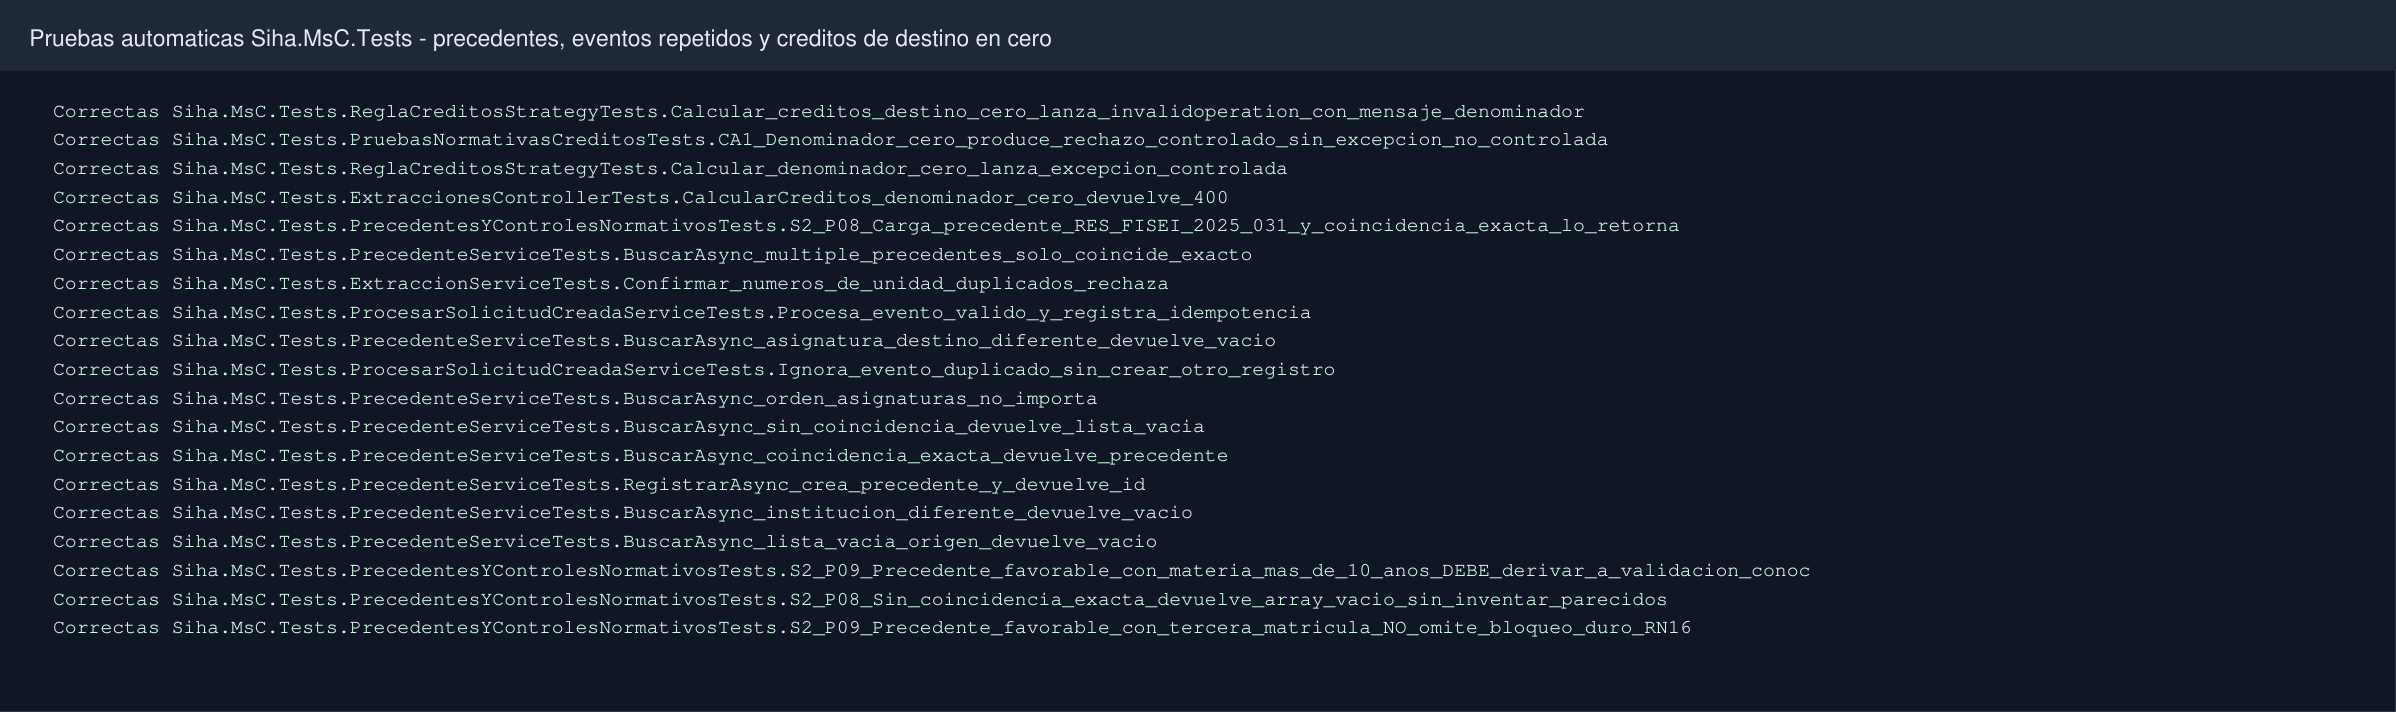
\includegraphics[width=\textwidth]{pa11-automaticas.png}
\caption{Pruebas automáticas de precedentes, avisos repetidos y créditos de destino en cero (HU-09 y HU-11)}
\label{fig:automaticas}
\end{figure}

\begin{table}[H]\centering\small
\begin{tabularx}{\textwidth}{|l|X|X|l|}\hline
\rowcolor{grisTarjeta}\textbf{N.º} & \textbf{Prueba} & \textbf{Resultado obtenido} & \textbf{Estado}\\\hline
PA-07.1 & Lectura de un PDF con texto & Datos completos del certificado & Cumple\\\hline
PA-07.2 & Aviso repetido & Aviso con enlace; un solo análisis & Cumple\\\hline
PA-07.3 & Datos que faltan & ``Campos sin llenar''; no se analiza & Cumple\\\hline
PA-07.4 & Confirmar con datos vacíos & Lista de faltantes; no se guarda & Cumple\\\hline
PA-07.5 & PDF escaneado & ``No es el certificado SIHA'' & Cumple\\\hline
PA-08.1 & Reglas en el resultado & Reglas explicadas por materia & Cumple\\\hline
PA-08.2 & Cambio de umbral & 85~\%, versión 5 (luego 80~\%) & Cumple\\\hline
PA-08.3 & Servicio apagado & ``Se está preparando'' y reintento & Cumple\\\hline
PA-09.1 & Créditos suficientes & 100~\% & Cumple\\\hline
PA-09.2 & Créditos insuficientes & 66,67~\%: no se puede homologar & Cumple\\\hline
PA-09.3 & Destino sin créditos & Rechazo controlado & Cumple (automática)\\\hline
PA-09.4 & Más de 10 años & Rechazado & Cumple\\\hline
PA-09.5 & Tercera matrícula & Regla explicada; bloqueo automático & Cumple\\\hline
PA-10.1 & Escaneado legible & Ya no se reciben escaneados & Reemplazada (C-01)\\\hline
PA-10.2 & Cobertura por unidades & Tabla tema por tema & Cumple\\\hline
PA-10.3 & Parecido bajo el umbral & Unidad no cubierta & Cumple\\\hline
PA-10.4 & Dos materias para un destino & Temas sumados & Cumple\\\hline
PA-10.5 & Misma materia en dos destinos & Rechazado & Cumple\\\hline
PA-11.1 & Coincidencia exacta & \texttt{BuscarAsync\_coincidencia\_exacta\dots} & Cumple (automática)\\\hline
PA-11.2 & Sin coincidencia & \texttt{BuscarAsync\_sin\_coincidencia\dots} & Cumple (automática)\\\hline
PA-11.3 & Caso solo parecido & \texttt{\dots solo\_coincide\_exacto} & Cumple (automática)\\\hline
PA-11.4 & Precedente y más de 10 años & \texttt{S2\_P09\_Precedente\_favorable\dots} & Cumple (automática)\\\hline
PA-11.5 & Falla la búsqueda & Cubierta por el reintento automático (PA-08.3) & Cumple (corregida C-03)\\\hline
\end{tabularx}
\caption{Resultados de las pruebas del Sprint 2 (nueva ejecución)}
\end{table}

% =====================================================================
\clearpage
\subsection{Sprint 3: revisión, decisión y resultado (HU-12 a HU-19)}

\subsubsection{HU-12 -- Registrar con un único certificado SIHA}

\prueba{PA-12.1: Solicitudes registradas}
{El administrador abre Solicitudes.}
{pa12-1-lista-solicitudes.png}{Lista de solicitudes con su estado (HU-12)}
{Cada solicitud muestra el estudiante, el cambio de carrera, las materias pedidas, los docentes revisores y su estado
(Revisión docente, Falta la decisión del administrador o Resuelta).}{0.95}

\prueba{PA-12.2: Revisión previa con lista de verificación}
{El operador sube el certificado E05, que pide homologar una materia reprobada.}
{pa12-2-checklist.png}{Lista de verificación por sección (HU-12)}
{Cada sección del certificado aparece con un visto o una equis y el motivo en lenguaje sencillo; el botón de registrar
queda deshabilitado y explica por qué.}{0.80}

\textbf{PA-12.3: Certificado repetido.} Se comprobó en la PA-07.2: el aviso aparece junto al botón con el enlace a la
solicitud que ya existe.

\subsubsection{HU-13 -- Análisis explicado con los sílabos oficiales}

\prueba{PA-13.1: Análisis materia por materia}
{Se abre la solicitud V05 recién registrada.}
{pa13-1-analisis.png}{Resumen y análisis explicado (HU-13)}
{El resumen indica cuántas materias cumplen y cuántas no se pueden homologar por créditos; cada materia trae su
recomendación, el historial y las reglas del instructivo.}{0.62}

\prueba{PA-13.2: Reintento automático}
{Tras encender de nuevo Ollama (PA-08.3) se vuelve a abrir la solicitud V07.}
{pa13-2-reintento-analizado.png}{La solicitud se analizó sola al volver el servicio (HU-13)}
{La solicitud pasó de ``El agente se está preparando'' a analizada, sin intervención del operador.}{0.95}

\subsubsection{HU-14 -- Movilidad externa}

\prueba{PA-14.1: Solicitud de otra universidad}
{Se abre la solicitud de movilidad externa de la ESPOCH (V06).}
{pa14-1-movilidad-externa.png}{Movilidad externa con sílabos de otra universidad (HU-14)}
{Las materias con sílabo adjunto se comparan con el de la UTA; las que no tienen sílabo quedan ``Sin sílabo para
comparar · decide el docente'' (criterio docente).}{0.95}

\subsubsection{HU-15 -- Regla: los créditos bloquean, los contenidos recomiendan}

\prueba{PA-15.1: Créditos por debajo del 80~\%}
{Se revisa Algoritmos y Lógica de Programación en la solicitud V05 (créditos 50~\%).}
{pa15-1-bloqueada-creditos.png}{Materia bloqueada por créditos (HU-15)}
{``No se puede homologar'' y ``Los créditos no llegan al 80~\%'': no hay botones de voto.}{0.95}

\prueba{PA-15.2: Solo contenidos por debajo del 80~\%}
{Se revisa Sistemas Operativos en la solicitud V03 (contenidos 75~\%, créditos 100~\%).}
{pa15-2-recomendacion.png}{Recomendación que los docentes pueden votar (HU-15)}
{``No llega al 80~\% · recomienda no homologar'', pero los docentes sí pueden votarla (ver PA-16.1).}{0.95}

\subsubsection{HU-16 -- Decisión de los docentes y del administrador}

\prueba{PA-16.1: Voto de un docente}
{La docente María Vaca decide las cuatro materias de V03 y rechaza Sistemas Operativos.}
{pa16-1-voto-docente.png}{Voto de una docente (HU-16)}
{El voto queda guardado con su comentario y la solicitud pasa a ``Revisión docente 1/2''.}{0.95}

\prueba{PA-16.2: Los docentes no coinciden}
{El docente Carlos Paredes aprueba Sistemas Operativos.}
{pa16-2-sin-acuerdo.png}{Docentes sin acuerdo (HU-16)}
{La solicitud pasa a ``Falta la decisión del administrador'' y los docentes ven el aviso del desacuerdo.}{0.95}

\prueba{PA-16.3: Decisión final del administrador}
{El administrador elige No homologar y escribe el motivo. Sin motivo el botón Guardar decisión final queda deshabilitado.}
{pa16-3-decision-admin-formulario.png}{Formulario de la decisión final (HU-16)}
{Solo aparece para la materia sin acuerdo y exige el motivo.}{0.95}

\prueba{PA-16.3 (continuación): Solicitud resuelta}
{El administrador guarda la decisión.}
{pa16-3-decision-admin.png}{Decisión final guardada (HU-16)}
{Sistemas Operativos queda No homologada con la decisión y el motivo del administrador; la solicitud pasa a Resuelta.}{0.95}

\prueba{PA-16.4: Cambiar el voto después de la decisión final}
{La docente María Vaca vuelve a la solicitud e intenta enviar otro voto directamente al servidor.}
{pa16-4-votos-cerrados.png}{Votos cerrados después de la decisión final (HU-16)}
{La pantalla ya no ofrece votar (``El administrador ya dio la decisión final'') y el servidor responde \textbf{409} con
``El administrador ya dio la decisión final de esta solicitud; los votos ya no se pueden cambiar.''}{0.95}

\subsubsection{HU-17 -- Tabla de resultados de la homologación}

\prueba{PA-17.1: Tabla RESULTADO\_HOMOLOGACION}
{Se consulta la tabla en la base del Microservicio C.}
{pa17-1-resultado-homologacion.png}{Resultado por materia en la base de datos (HU-17)}
{Una fila por materia con los porcentajes de contenidos y créditos, la estimación del agente, los votos y el resultado
final; coincide con lo que se ve en la aplicación (por ejemplo, Álgebra Lineal 100~\% / 66,67~\% NO\_HOMOLOGADA y
Sistemas Operativos 1--1 NO\_HOMOLOGADA por decisión del administrador).}{1.0}

\subsubsection{HU-18 -- Registro manual sin PDF}

\prueba{PA-18.1: Llenado automático desde la malla}
{El operador elige Ingeniería Industrial a Software, pulsa Cargar materias de la malla hasta el nivel 2 y elige el período de la primera materia de cada nivel.}
{pa18-1-carga-automatica.png}{Historial cargado desde la malla de origen (HU-18)}
{Se cargan solas las 12 materias de los niveles 1 y 2. El nivel y la materia se eligen de listas, y el período se elige de los períodos de la UTA ya precargados: al elegirlo en una materia se copia a las demás del mismo nivel. Solo falta escribir la nota.}{0.95}

\prueba{PA-18.2: Materias que no se relacionan}
{El operador pide homologar Química por Algoritmos y Lógica de Programación.}
{pa18-2-no-relacionadas.png}{Aviso de materias que no se relacionan y sugerencias (HU-18)}
{Aparece ``Estas materias no se relacionan: «Quimica» no se relaciona con «Algoritmos y logica de programacion» (sus
temas se parecen solo un 2~\%)'' y se ofrecen sugerencias automáticas con materias parecidas.}{0.95}

\subsubsection{HU-19 -- Cuentas y sesión}

\prueba{PA-19.1: Restablecer contraseña}
{El administrador pulsa Restablecer contraseña en la cuenta del operador.}
{pa19-1-restablecer.png}{Restablecer la contraseña de una cuenta (HU-19)}
{Se abre la ventana con nueva contraseña, confirmación y el botón Mostrar; solo el Administrador la ve.}{0.95}

\textbf{PA-19.2: Volver a una página permitida al iniciar sesión.} Lo comprueban las pruebas automáticas de
\texttt{navegacion.test.ts} y \texttt{LoginPage}: después de iniciar sesión solo se vuelve a la página anterior si el
rol la puede ver.

\begin{table}[H]\centering\small
\begin{tabularx}{\textwidth}{|l|X|X|l|}\hline
\rowcolor{grisTarjeta}\textbf{N.º} & \textbf{Prueba} & \textbf{Resultado obtenido} & \textbf{Estado}\\\hline
PA-12.1 & Solicitudes registradas & Lista con estados & Cumple\\\hline
PA-12.2 & Revisión previa & Lista de verificación por sección & Cumple\\\hline
PA-12.3 & Certificado repetido & Aviso con enlace & Cumple\\\hline
PA-13.1 & Análisis explicado & Resumen y explicación por materia & Cumple\\\hline
PA-13.2 & Reintento automático & Se analizó sola & Cumple\\\hline
PA-14.1 & Movilidad externa & Sílabo externo y criterio docente & Cumple\\\hline
PA-15.1 & Créditos bajo 80~\% & Bloqueada, sin voto & Cumple\\\hline
PA-15.2 & Solo contenidos bajo 80~\% & Recomendación votable & Cumple\\\hline
PA-16.1 & Voto de un docente & Revisión 1/2 & Cumple\\\hline
PA-16.2 & Sin acuerdo & Falta la decisión del administrador & Cumple\\\hline
PA-16.3 & Decisión final & Con motivo; solicitud Resuelta & Cumple\\\hline
PA-16.4 & Votos cerrados & Pantalla sin voto y 409 & Cumple\\\hline
PA-17.1 & Tabla de resultados & Filas coherentes con la app & Cumple\\\hline
PA-18.1 & Llenado automático & 12 materias y períodos precargados & Cumple\\\hline
PA-18.2 & Materias no relacionadas & Rechazo y sugerencias & Cumple\\\hline
PA-19.1 & Restablecer contraseña & Ventana solo para Administrador & Cumple\\\hline
PA-19.2 & Página permitida al entrar & Pruebas de navegación & Cumple (automática)\\\hline
\end{tabularx}
\caption{Resultados de las pruebas del Sprint 3}
\end{table}

% =====================================================================
\subsection{Hallazgos de la ronda de pruebas}

\begin{table}[H]\centering\small
\begin{tabularx}{\textwidth}{|l|l|X|l|}\hline
\rowcolor{grisTarjeta}\textbf{ID} & \textbf{Gravedad} & \textbf{Descripción} & \textbf{Estado}\\\hline
H-01 & Baja & El resumen decía ``recomienda no homologar'' para materias bloqueadas por créditos. & Corregido\\\hline
H-02 & Media & La regla RN-01 del catálogo todavía decía que los docentes podían homologar aunque no se llegue. & Corregido (RN-01 2.2)\\\hline
H-03 & Media & En el registro manual, ``Agregar todas las sugerencias'' crea las solicitudes pero deja vacía la materia de destino (diferencia de mayúsculas entre la sugerencia y la lista). & Corregido\\\hline
H-04 & Baja & La página ``Reglas de homologación'' (explicación sencilla) ya no está en el menú ni en las rutas. & Pendiente (decisión del equipo)\\\hline
H-05 & Baja & En el Microservicio B el expediente queda en PENDIENTE\_CONTENIDOS aunque en el C ya esté resuelto. & Pendiente\\\hline
H-06 & Baja & El catálogo muestra los nombres de las materias sin tildes (por ejemplo ``Quimica'', ``Fisica basica''). & Pendiente\\\hline
\end{tabularx}
\caption{Hallazgos encontrados al ejecutar las pruebas}
\end{table}

\begin{figure}[H]\centering
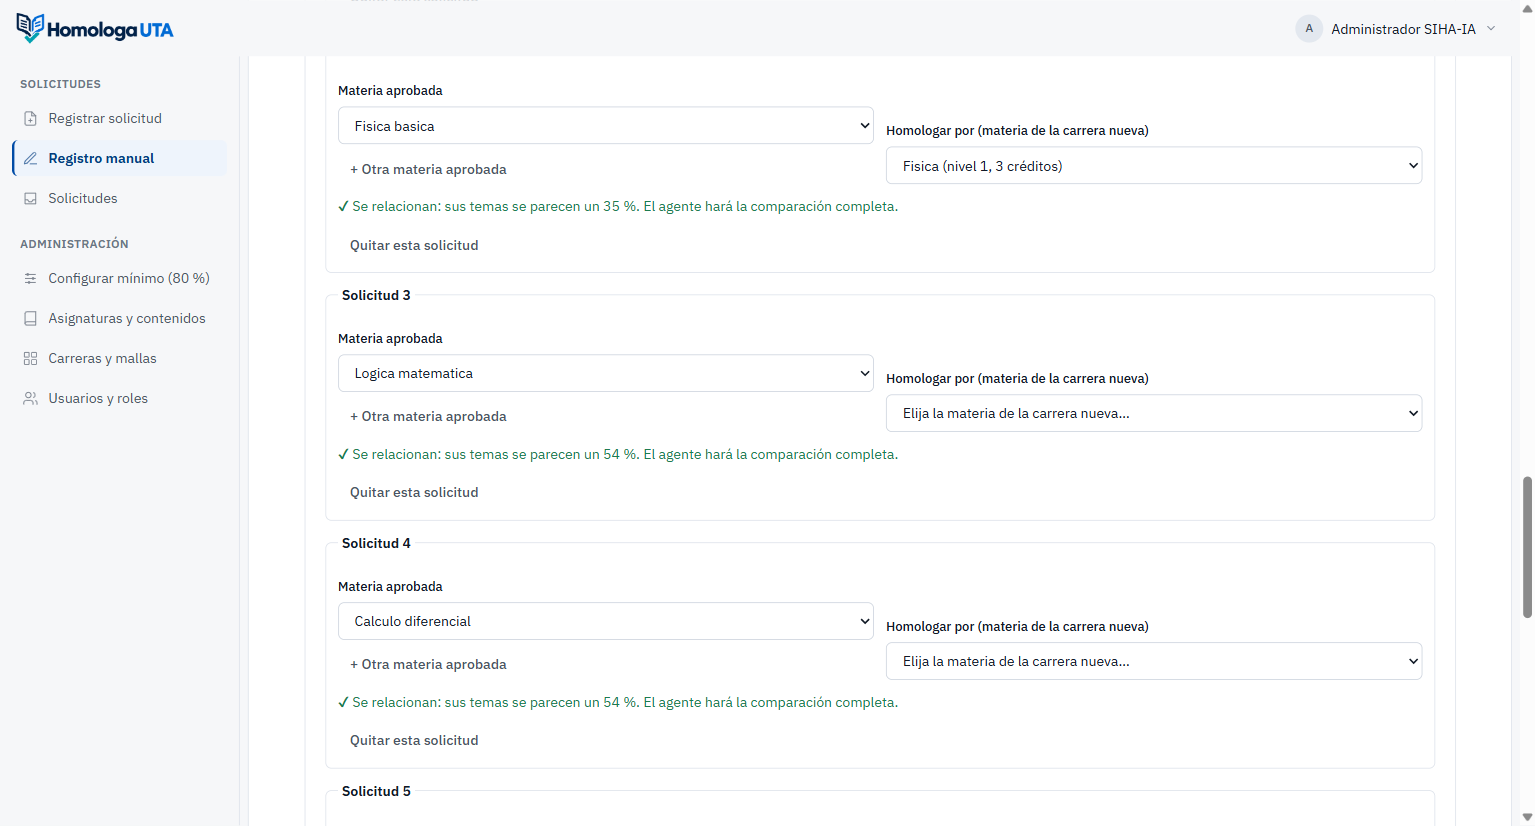
\includegraphics[width=0.85\textwidth]{h-sugerencias-destino-vacio.png}
\caption{Hallazgo H-03 antes de corregirlo: solicitudes sugeridas con la materia de destino vacía}
\end{figure}

La causa de H-03 era que la sugerencia trae el nombre de la materia con otras mayúsculas o sin tildes, y la lista no lo reconocía. Se corrigió para que se elija la materia de la malla que tiene el mismo nombre, y se agregó una prueba automática que lo comprueba.

\begin{figure}[H]\centering
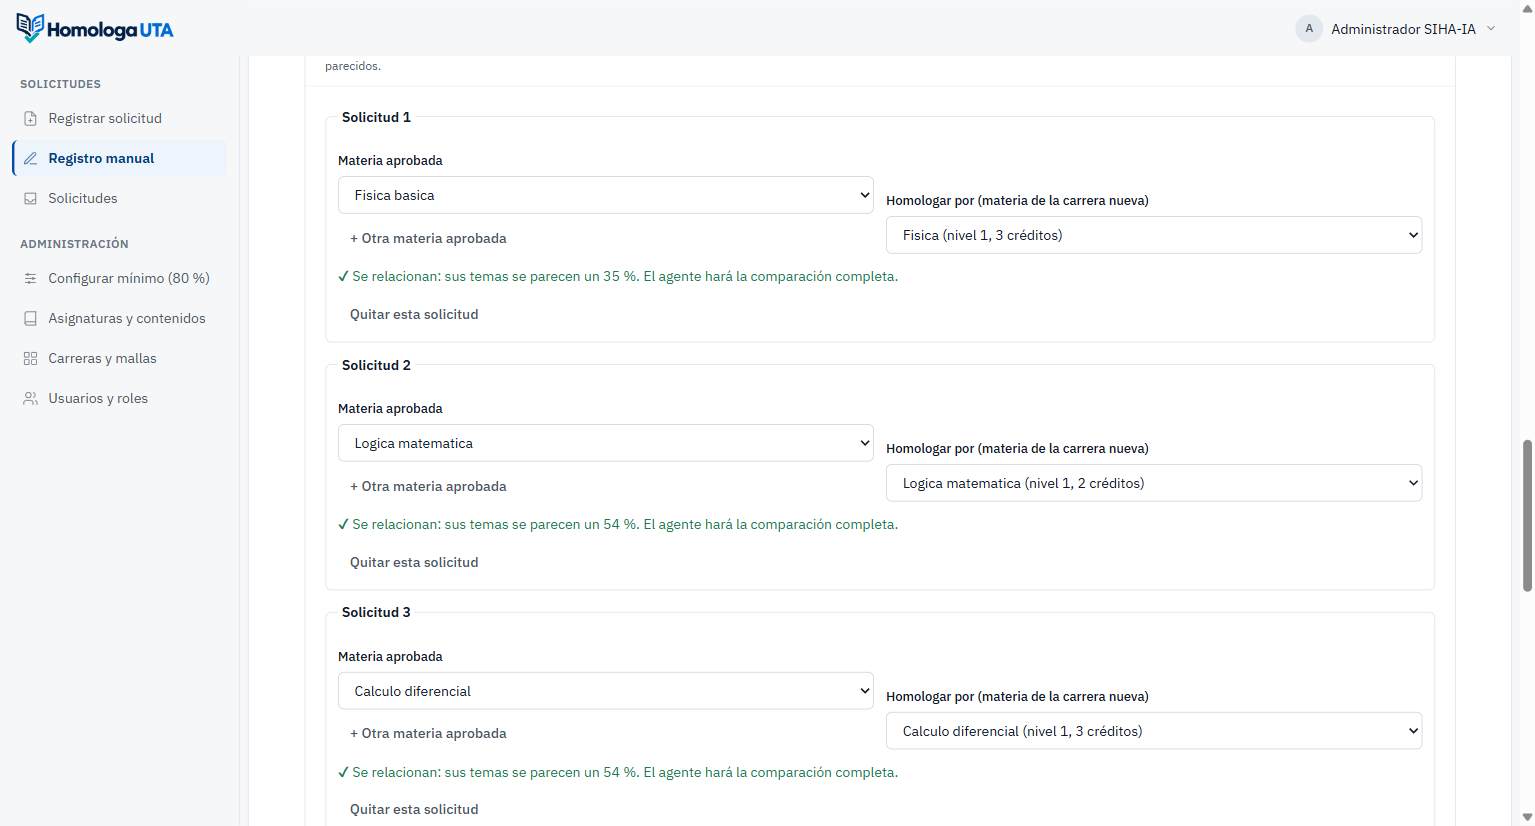
\includegraphics[width=0.85\textwidth]{h-sugerencias-destino-corregido.png}
\caption{Hallazgo H-03 corregido: cada solicitud sugerida ya tiene su materia de destino}
\end{figure}

% =====================================================================
\subsection{Pruebas automáticas}

\begin{table}[H]\centering\small
\begin{tabular}{|l|l|r|l|}\hline
\rowcolor{grisTarjeta}\textbf{Proyecto} & \textbf{Herramienta} & \textbf{Pruebas} & \textbf{Resultado}\\\hline
Microservicio A (usuarios, reglas, catálogo) & xUnit & 130 & Todas correctas\\\hline
Microservicio B (expedientes y certificado) & xUnit & 158 & Todas correctas\\\hline
Microservicio C (agente y decisión) & xUnit & 257 & Todas correctas\\\hline
Interfaz web & Vitest & 99 & Todas correctas\\\hline
Gateway (rutas y permisos) & Node & 26 & Todas correctas\\\hline
\end{tabular}
\caption{Pruebas automáticas al cierre del Sprint 3}
\end{table}

\subsection{Resumen general}

\begin{table}[H]\centering\small
\begin{tabular}{|l|c|c|c|c|}\hline
\rowcolor{grisTarjeta}\textbf{Estado} & \textbf{Sprint 1} & \textbf{Sprint 2} & \textbf{Sprint 3} & \textbf{Total}\\\hline
Cumple & 12 & 16 & 16 & 44\\\hline
Cumple (automática) & 0 & 5 & 1 & 6\\\hline
Cumple (corregida) & 0 & 1 & 0 & 1\\\hline
Reemplazada por una corrección & 0 & 1 & 0 & 1\\\hline
Pendiente & 0 & 0 & 0 & 0\\\hline
\textbf{Total} & \textbf{12} & \textbf{23} & \textbf{17} & \textbf{52}\\\hline
\end{tabular}
\caption{Resumen de los resultados de las pruebas de los tres sprints}
\end{table}

Todas las capturas originales están en la carpeta \texttt{capturas}, nombradas por prueba y en el mismo orden de esta sección.

\section{Declaración de uso de inteligencia artificial}
Durante el Sprint 3 el equipo usó herramientas de inteligencia artificial generativa, entre ellas Claude Code y Codex, para escribir gran parte del código, generar pruebas automáticas, revisar errores y preparar este informe. Los integrantes revisaron el código y los resultados, ejecutaron las pruebas automáticas y la integración continua, y realizaron la ronda de pruebas manuales descrita en la sección 10. La IA local Ollama forma parte del sistema SIHA como apoyo para analizar materias; no se usó como herramienta de desarrollo.

\section{Conclusión y próximos pasos}
El Sprint 1 entregó la base del sistema: cuentas, permisos, reglas, catálogo y flujo inicial de expedientes. El Sprint 2 incorporó la lectura del plan, el análisis de créditos y contenidos, la explicación de resultados y la consulta de precedentes, además de sus correcciones posteriores. El Sprint 3 completó el flujo con el certificado SIHA único, la revisión previa, los sílabos oficiales y externos, las recomendaciones por materia, los votos de dos docentes, la decisión administrativa cuando discrepan, el registro manual y los resultados consultables.

La regla quedó aclarada con el docente: si los créditos están bajo el 80~\%, la materia queda bloqueada; si los contenidos están bajo el 80~\%, el agente recomienda no homologar, pero los docentes pueden decidir con su criterio. El agente no sustituye la revisión de los docentes.

El hallazgo H-03, en el que las sugerencias dejaban vacía la materia de destino, ya quedó corregido. Los siguientes pasos son decidir si se recupera H-04, la página de reglas; sincronizar el estado del expediente en MS B cuando MS C lo resuelve (H-05); y mostrar con tildes los nombres del catálogo (H-06). También quedan por evaluar los avisos por correo y cargar los sílabos de Robótica para los niveles 6 a 9.


\end{document}
